% 제4장 연구 결과
% 1차 심사 반영: 구 제3장 결과 부분(3.2--3.8) + 구 제4장 교차분석(4.1--4.6) 통합
% 3차 심사 반영: 파일명을 실제 절 번호와 일치시키도록 정리 (2026-05-09)

\chapter{\vrev{연구 결과}}
\label{ch:results}

\vrev{%
본 장에서는 4단계 조건 체계(C0--C3)별 시뮬레이션 결과를 순차적으로 보고하고,
\chg{회귀분석, 강건성, 수렴 진단}을 통해 모델의 통계적 타당성을 검증한다.
이어서 가설 검증 종합과 조건 간 교차분석(효과 크기, 회귀 설명력,
이중채널 감쇠), 전문가 검증 결과, 선행연구와의 교차 정합성을 제시한다.
}
% 3차 심사 (2026-05-09): 파일명을 실제 절 번호와 일치시키기 위해 ch4 7개 파일 일괄 rename.
% sec4.7_hypothesis → sec4.13_hypothesis (실제 4.13절)
% sec4.8_c2_c3_synthesis → sec4.7_c2_c3_synthesis (실제 4.7절)
% sec4.9_effect_size → sec4.8_effect_size, sec4.10_r2_progression → sec4.9_r2_progression
% sec4.11_dual_channel → sec4.10_dual_channel, sec4.12_expert_verify → sec4.11_expert_verify
% sec4.13_cross_consistency → sec4.12_cross_consistency

% 조건별 시뮬레이션 결과


%% ===================================================================
\section{\vrev{C0와 C1의 관측성 효과}}
\label{sec:result_c0c1}
%% ===================================================================

%% -------------------------------------------------------------------
\subsection{\vrev{정적 기준선 C0}}
\label{subsec:result_c0}
%% -------------------------------------------------------------------

\textbf{C0} 조건은 관측성과 불확실성이 모두 비활성화된 정적 기준선으로서,
$O_{\text{raw}}$, $k_O$, $U_{\text{raw}}$가 모델에 입력되지 않아
$z_O = 0$, $z_U = 0$이 고정된다. 이 경우 개별 시그모이드 바운딩 함수의
인자가 $S(0) = 0$이 되어, $\DRTO = R_0 = 6.0$시간이
결정론적으로 산출된다.

따라서 효율성 비율은 $\eta_{\text{C0}} = \DRTO / R_0 = 1.000$이며,
표준편차 $\mathrm{SD} = 0.000$, 모든 표본에서 동일한 값이 관측된다.
C0는 확률적 변동이 존재하지 않는 기준점으로서, C1 이후 조건에서
나타나는 변동의 크기와 방향을 평가하기 위한 앵커(anchor) 역할을 수행한다.


%% -------------------------------------------------------------------
\subsection{\vrev{C1의 관측성 기반 동적 조정}}
\label{subsec:result_c1}
%% -------------------------------------------------------------------

\textbf{C1} 조건은 관측성($O$, $k_O$)만 활성화하고 불확실성을 비활성화한
상태($z_U = 0$)로, 관측성이 $\DRTO$에 미치는 순수한 효과를 분리하여
관측하는 조건이다.
$\kappa = 1.2$에서 관측성 바운딩 효과 $E_{O,\text{bnd}} = -R_0 \cdot S(\kappa \cdot k_O \cdot O_{\text{raw}})$만
활성화되어, $\DRTO = R_0 + E_{O,\text{bnd}} \leq R_0$가 보장된다.

\chg{기술통계 측면에서,} C1 조건의 효율성 비율 평균은 $\bar{\eta}_{\text{C1}} = 0.853$,
$\mathrm{SD} = 0.125$로 나타났다.
C0의 결정론적 $\eta = 1.000$ 대비 $14.7\%$가 감소한 것으로,
$\DRTO$ 평균은 $5.115$시간이다.
관측성이 도입되면 $\DRTO$가 기본 복구시간 $R_0$보다 체계적으로 단축됨을 의미하며,
이러한 단축 효과는 관측성이 높을수록 이상 징후의 조기 탐지를 통해
복구 시간을 절감할 수 있다는 실무적 논리와 일치한다.

\chg{효과 크기 측면에서,} C0 대비 C1의 Cohen's $d = -1.180$로서, 이는 \citet{cohen1988power}의
기준에 따라 \textbf{대효과(large effect)}에 해당한다(대효과 기준값 $|d|=0.80$의 약 $1.48$배).
방향이 음(-)인 것은 관측성 도입이 $\eta$를 감소(즉, 복구 시간 단축)
시킨다는 것을 나타낸다.
$n = 10{,}000$개 표본 전체에서 $\eta_{\text{C1}} \leq \eta_{\text{C0}}$인
비율이 $100\%$로(\jrev{H3}-a), 관측성의 복구 단축 효과가 예외 없이
관찰되었다. 이는 H1(관측성 효과 가설)의 충족을 실증적으로 확인한다.


%% -------------------------------------------------------------------
\subsection{\vrev{C0/C1 분포 시각화}}
\label{subsec:c0c1_visual}
%% -------------------------------------------------------------------

\figref{fig:eta_c0c1_hist}\refpo{fig:eta_c0c1_hist}{은}{는} C0와 C1 조건의 $\eta$ 분포를 비교한 것이다.
C0는 $\eta = 1.000$에서의 단일 수직선으로 표현되며,
C1은 $[0.468,\;1.000]$ 구간에서 좌측으로 치우친 분포를 형성한다.
\chg{그림에서 적색 점선은 C0 정적 기준선을, 청색 곡선은 C1 관측성 분포의 정규 근사를 나타낸다.}

\begin{figure}[htbp]
  \centering
  \begin{tikzpicture}
    \begin{axis}[
      width=0.9\textwidth,
      height=7cm,
      xlabel={효율성 비율 $\eta$},
      ylabel={밀도 (density)},
      xmin=0.3, xmax=2.2,
      ymin=0,
      ymajorgrids=true,
      grid style={dashed, black},
      legend style={at={(0.98,0.95)}, anchor=north east, font=\small},
      legend cell align=left,
      ]
      % C0: vertical line at eta=1.0
      \addplot[red, ultra thick, dashed, domain=0:8, samples=2]
        coordinates {(1.0,0) (1.0,7.5)};
      \addlegendentry{C0 ($\eta = 1.000$)}

      % C1: approximate density using beta-like shape (mean=0.853, SD=0.125)
      % Skewed left distribution
      \addplot[blue, thick, smooth, domain=0.4:1.0, samples=100]
        {3.2*exp(-0.5*((x-0.853)/0.125)^2)};
      \addlegendentry{C1 ($\bar{\eta} = 0.853$)}

      % 우측 하단 메모: C1 범위 및 산출 근거
      \node[anchor=south east, font=\footnotesize, align=left,
            text=black] at (rel axis cs:0.97,0.03)
        {C1: $\eta \in [0.468,\;1.000]$\\
         $\eta_{\min} = \DRTO_{\min}/R_0 = 2.810/6.0 = 0.468$\\
         $z_{O,\max} = \kappa \cdot k_O \cdot O_{\text{raw}} = 1.2 \times 1 \times 1$};
    \end{axis}
  \end{tikzpicture}
  \caption{C0/C1 조건의 효율성 비율 $\eta$ 분포 비교}
  \label{fig:eta_c0c1_hist}
\end{figure}

\chg{끝으로 H1의 검증 결론을 검증한다.} \mrev{H1은 ``$\DRTO_{\text{C1}} \leq R_0 = 6.0$h가 100\% 표본에서 성립''을
판정 기준으로 한다. $n = 10{,}000$ 표본 전체에서 $\eta_{\text{C1}} \in
[0.468, 1.000]$로 1.0을 초과하는 사례가 0건이며, 순서 준수율이 100.0\%로
H3-a와 결합하여 관측성의 복구 단축 효과가 결정론적으로 확인된다. 효과
크기 Cohen's $d = -1.180$ (매우 큰 효과; \secref{sec:ch5_effect_size}
참조)이 동시에 충족되어, \textbf{H1은 채택된다}.}

\chg{이어 H3-a의 검증 결론은 다음과 같다.} \mrev{H3-a는 ``$\eta_{\text{C1}} \leq \eta_{\text{C0}} = 1.0$인 비율
$\geq 99\%$''를 기준으로 한다. $n = 10{,}000$ 전체에서 100.0\%가 충족되어,
\textbf{H3-a는 채택된다}.}
        % 4.1 C0/C1 결과


%% ===================================================================
\section{\vrev{C2 가우시안 불확실성 결과}}
\label{sec:result_c2}
%% ===================================================================

\textbf{C2} 조건은 C1의 관측성에 가우시안 불확실성($U_{\text{raw}}^{(G)} \sim N(3,1)$)을
추가한 것으로, 경꼬리(light-tail, 가우시안) 불확실성이 $\DRTO$에 미치는 효과를
관측하는 조건이다.
개별 시그모이드 바운딩 모델에서 $E_{O,\text{bnd}}$와 $E_{U,\text{bnd}}$가
각각 독립적으로 바운딩되므로,
$\DRTO = R_0 + E_{O,\text{bnd}} + E_{U,\text{bnd}}$의 구조가
관측성의 하향 효과와 불확실성의 상향 효과를 명확히 분리한다.

\figref{fig:gaussian_concept}\refpo{fig:gaussian_concept}{은}{는} 가우시안 불확실성의 분포 특성과
시그모이드 바운딩을 통한 $\DRTO$ 상향 조정 메커니즘을 개념적으로 도식화한 것이다.
\chg{패널 (a)는 평균 $\mu = 3.0$의 대칭적 확률밀도함수 $N(3,1)$을, 패널 (b)는 불확실성 수준에 따른
$\DRTO$의 상향 조정을 보이며, 시그모이드 바운딩에 의해 $R_0 < \DRTO < R_{\max}$가 보장되어 높은
$U$ 영역에서 자연스럽게 포화한다.}

\begin{figure}[htbp]
  \centering
  \begin{tikzpicture}
    % ── Panel (a): Gaussian N(3,1) PDF ──
    \begin{axis}[
      name=panelA,
      width=0.47\textwidth,
      height=6.5cm,
      xlabel={$U_{\text{raw}}$ (불확실성 수준, 시간)},
      ylabel={확률밀도},
      title={\textbf{(a)} 가우시안 불확실성 $U \sim N(3, 1)$},
      title style={font=\small\bfseries},
      xmin=-1, xmax=7,
      ymin=0, ymax=0.46,
      ymajorgrids=true,
      grid style={dashed, black},
      legend style={at={(0.02,0.98)}, anchor=north west, font=\scriptsize},
      ]
      % Gaussian PDF (approximated with smooth curve)
      \addplot[blue!70!black, thick, smooth, domain=-1:7, samples=100]
        {1/(sqrt(2*pi)*1)*exp(-0.5*((x-3)/1)^2)};
      \addlegendentry{$N(3, 1)$}

      % Mean line
      \draw[red!70!black, dashed, thick] (axis cs:3, 0) -- (axis cs:3, 0.40);
      \node[font=\scriptsize, red!70!black, fill=white, inner sep=1.5pt,
            rounded corners=1pt] at (axis cs:3, 0.44) {$\mu = 3.0$};

      % ±1σ lines
      \draw[black, dotted, thin] (axis cs:2, 0) -- (axis cs:2, 0.245);
      \draw[black, dotted, thin] (axis cs:4, 0) -- (axis cs:4, 0.245);
      \node[font=\tiny, black] at (axis cs:5.5, 0.26) {$\pm 1\sigma$: 68.3\%};
      \draw[-{Stealth}, black, thin] (axis cs:5.2, 0.25) -- (axis cs:4.1, 0.24);

      % Symmetry annotation
      \node[font=\tiny, black, align=center] at (axis cs:-0.2, 0.30) {대칭 분포\\(Skewness $= 0$)};
    \end{axis}

    % ── Panel (b): DRTO shift via sigmoid bounding ──
    \begin{axis}[
      at={(panelA.east)},
      anchor=west,
      xshift=18mm,
      width=0.47\textwidth,
      height=6.5cm,
      xlabel={$U_{\text{raw}}$ (불확실성 수준, 시간)},
      ylabel={$\DRTO$ (시간)},
      title={\textbf{(b)} 시그모이드 바운딩에 의한 불확실성 프리미엄},
      title style={font=\small\bfseries},
      xmin=0, xmax=8,
      ymin=5.0, ymax=25,
      ymajorgrids=true,
      grid style={dashed, black},
      legend style={at={(0.98,0.98)}, anchor=north east, font=\scriptsize},
      ]
      % DRTO = R0 + E_U,bnd = R0 + (Rmax-R0)·S(κ·U/6)
      % S(z) = 2/(1+exp(-z)) - 1
      \addplot[red!70!black, thick, smooth, domain=0:8, samples=100]
        {6.0 + 18.0*(2/(1+exp(-1.2*x/6)) - 1)};
      \addlegendentry{$R_0 + E_{U,\text{bnd}}$}

      % R0 baseline
      \draw[black, dashed, thick] (axis cs:0, 6.0) -- (axis cs:8, 6.0);
      \node[font=\tiny, black] at (axis cs:1.0, 6.5) {$R_0 = 6.0$h};

      % Rmax upper bound
      \draw[black, dotted, thin] (axis cs:0, 24.0) -- (axis cs:8, 24.0);
      \node[font=\tiny, black] at (axis cs:1.0, 24.5) {$R_{\max} = 24.0$h};

      % Mean point
      \addplot[only marks, mark=*, mark size=2.5pt, red!70!black]
        coordinates {(3.0, {6.0 + 18.0*(2/(1+exp(-1.2*3.0/6)) - 1)})};
      \node[font=\tiny, red!70!black, fill=white, inner sep=1pt, rounded corners=1pt,
            anchor=north west] at (axis cs:3.3, 9.0)
        {$U_{\text{raw}} = \mu\;(3.0)$};

      % Saturation annotation
      \node[font=\tiny, blue!70!black, align=center, fill=white, inner sep=1pt,
            rounded corners=1pt] at (axis cs:6.5, 19)
        {시그모이드 포화\\($< R_{\max}$)};
      \draw[-{Stealth}, blue!70!black, thin] (axis cs:6.5, 18.2) -- (axis cs:6.5, 16.5);
    \end{axis}
  \end{tikzpicture}
  \caption{가우시안 불확실성 개념도}
  \label{fig:gaussian_concept}
\end{figure}


%% -------------------------------------------------------------------
\subsection{\vrev{기술통계 및 효과 크기}}
\label{subsec:c2_descriptive}
%% -------------------------------------------------------------------

\chg{기술통계 측면에서,} C2 조건의 효율성 비율 평균은 $\bar{\eta}_{\text{C2}} = 1.682$,
$\mathrm{SD} = 0.615$로 나타났다.
$\DRTO$ 평균은 $10.094$시간으로서, 기준선 $R_0 = 6.0$시간 대비
$68.2\%$가 증가하였다.
C1의 $\bar{\eta} = 0.853$ 대비 $\erf{0.829}{0.830}$가 상승한 것으로,
불확실성의 도입이 $\eta$를 $1.0$ 이상으로
끌어올리는 \textbf{불확실성 프리미엄(uncertainty premium)} 효과를
확인하였다. 즉, 불확실성이 존재하는 환경에서 $\DRTO$는 기본 복구 시간
$R_0$보다 길어지며, 이는 복구 과정의 불확실성을 사전에 반영한
안전 마진(safety margin)으로 해석된다.

\chg{불확실성 프리미엄 비율을 보면,} 전체 $n = 10{,}000$개 표본 중 $\eta_{\text{C2}} > 1.0$인 비율,
즉 $\DRTO$가 기준선 $R_0$를 초과하는 비율은 $84.9\%$이다.
이는 가우시안 불확실성이 존재하는 환경에서 약 $85\%$의 시나리오가
기준선보다 긴 복구 시간을 필요로 함을 의미하며,
불확실성 프리미엄이 예외적 현상이 아닌 \textit{일반적 현상}임을 보여준다.
나머지 $15.1\%$는 관측성이 매우 높은($k_O \approx 1$, $O_{\text{raw}} \approx 1$) 조합에서
발생하는 것으로, 높은 관측성이 불확실성 프리미엄을 상쇄할 수 있는
조건을 나타낸다.

\chg{효과 크기 측면에서,} C1 대비 C2의 Cohen's $d = +1.871$으로서, \textbf{대효과(large effect)}에
해당한다(대효과 기준값 $|d|=0.80$의 약 $2.34$배).
방향이 양(+)인 것은 불확실성 추가가 $\eta$를 증가(복구 시간
연장)시킨다는 것을 나타내며, C0$\to$C1의 감소 방향($d = -1.180$)과
대조를 이룬다. 이러한 방향 반전은 관측성의 단축 효과와 불확실성의
연장 효과가 구조적으로 상반됨을 보여주며,
개별 시그모이드 바운딩 모델의 이론적 설계가 실험적으로 타당함을 입증한다.


%% -------------------------------------------------------------------
\subsection{\vrev{순서 준수 및 가설 검증}}
\label{subsec:c2_order}
%% -------------------------------------------------------------------

$n = 10{,}000$개 표본 중 $\eta_{\text{C1}} \leq \eta_{\text{C2}}$인
비율이 $99.87\%$로(\jrev{H3}-b), C2의 불확실성 프리미엄은 거의 모든
표본에서 관찰되었다. $0.13\%$의 예외는 관측성이 매우 높고($O_{\text{raw}} \approx 1$,
$k_O \approx 1$) 불확실성이 매우 낮은($U_{\text{raw}}^{(G)} \approx 0$) 극단적 조합에서
발생하는 것으로, 모델의 구조적 특성과 일치한다.
\jrev{H3}-b의 기준($\geq 99\%$)을 $99.87\%$로 충족한다.

\chg{C2의 순서 준수에 대한 H3-b의 검증 결론은 다음과 같다.} \mrev{H3-b는 ``$\eta_{\text{C1}} \leq \eta_{\text{C2}}$ 비율 $\geq 99\%$''를
기준으로 한다. 99.87\%가 충족되어 ($0.13\%$ 예외는 $O_{\text{raw}} \approx 1$
극단 영역), \textbf{H3-b는 채택된다}.}
          % 4.2 C2 결과


%% ===================================================================
\section{\vrev{파레토 불확실성 환경의 C3 결과}}
\label{sec:result_c3}
%% ===================================================================

\textbf{C3} 조건은 C2의 가우시안 불확실성을 파레토 분포
($U_{\text{raw}}^{(P)} \sim 6 \cdot \mathrm{Pareto}(\alpha=3)$)로 대체한 것으로,
극단 사건(extreme events)이 $\DRTO$에 미치는 구조적 영향을
관측하는 핵심 조건이다.

\figref{fig:pareto_concept}\refpo{fig:pareto_concept}{은}{는} 가우시안과 파레토 분포의 확률밀도함수 비교 및
생존함수(survival function)를 통한 꼬리 행동의 질적 차이를 도식화한 것이다.
\chg{여기서 생존함수 $\bar{F}(u) = P(U > u) = 1 - F(u)$는 확률변수 $U$가 특정 값 $u$를 초과할 확률을
나타내며, 예컨대 $\bar{F}(10) = 0.01$이면 불확실성이 10시간을 초과할 확률이 1\%임을 의미한다. 생존함수
값이 높을수록 해당 수준 이상의 극단 사건이 빈번함을 뜻하며, 분포의 꼬리가 얼마나 느리게 감소하는지를
직접 비교할 수 있다.}
두 분포는 동일한 기대값 $E[U] = 3.0$을 공유하지만,
파레토 꼬리는 가우시안의 지수적 감쇠에 비해
극단 영역에서 현저히 높은 초과 확률을 나타낸다.
\chg{그림에서 패널 (a)는 동일 평균 $E[U] = 3.0$ 하의 확률밀도함수 비교를, 패널 (b)는 로그 스케일
생존함수 비교를 보인다. 가우시안의 지수적 감쇠($\sim e^{-x^2/2}$)에 비해 파레토 감쇠는 멱법칙($\sim x^{-3}$)을
따르며, 그 결과 P99에서 $U_{\text{raw}}$ 원시값은 가우시안 $5.326$, 파레토 $21.85$로 약 $4.1$배 차이를 보인다.}

\begin{figure}[htbp]
  \centering
  \begin{tikzpicture}
    % ── Panel (a): Gaussian vs Pareto PDF ──
    \begin{axis}[
      name=panelA,
      width=0.47\textwidth,
      height=6.5cm,
      xlabel={$U_{\text{raw}}$ (불확실성 수준, 시간)},
      ylabel={확률밀도},
      title={\textbf{(a)} 가우시안 vs.\ 파레토: 확률밀도함수 비교},
      title style={font=\small\bfseries},
      xmin=0, xmax=15,
      ymin=0, ymax=0.46,
      ymajorgrids=true,
      grid style={dashed, black},
      legend style={at={(0.98,0.88)}, anchor=north east, font=\scriptsize},
      ]
      % Gaussian N(3,1) PDF
      \addplot[blue!70!black, thick, smooth, domain=0:15, samples=120]
        {1/(sqrt(2*pi)*1)*exp(-0.5*((x-3)/1)^2)};
      \addlegendentry{Gaussian $N(3, 1)$}

      % Pareto PDF: f_Y(y) = α/(y/6+1)^(α+1) / 6, α=3
      \addplot[red!70!black, thick, smooth, domain=0.01:15, samples=120]
        {3.0 / ((x/6+1)^4) / 6.0};
      \addlegendentry{Pareto $6 \cdot \mathrm{Pareto}(3)$}

      % Mean line
      \draw[black, dashed, thick] (axis cs:3, 0) -- (axis cs:3, 0.42);
      \node[font=\scriptsize, black, fill=white, inner sep=1.5pt,
            rounded corners=1pt] at (axis cs:3, 0.44)
        {$E[U] = 3.0$h (동일 평균)};

      % Heavy tail annotation
      \node[font=\tiny, red!70!black, align=center, fill=white, inner sep=1pt,
            rounded corners=1pt] at (axis cs:11.5, 0.08)
        {중꼬리(파레토)\\멱법칙 감쇠};

      % Light tail annotation
      \node[font=\tiny, blue!70!black, align=center, fill=white, inner sep=1pt,
            rounded corners=1pt] at (axis cs:7.0, 0.16)
        {경꼬리(가우시안)\\지수적 감쇠};
    \end{axis}

    % ── Panel (b): Survival function (log scale) ──
    \begin{axis}[
      at={(panelA.east)},
      anchor=west,
      xshift=18mm,
      width=0.47\textwidth,
      height=6.5cm,
      xlabel={$U_{\text{raw}}$ (불확실성 수준, 시간)},
      ylabel={$P(U > u)$ (생존함수)},
      title={\textbf{(b)} 꼬리 행동: 생존함수 비교 (로그 스케일)},
      title style={font=\small\bfseries},
      xmin=0, xmax=20,
      ymode=log,
      ymin=1e-6, ymax=1.1,
      ymajorgrids=true,
      grid style={dashed, black},
      legend style={at={(0.98,0.98)}, anchor=north east, font=\scriptsize},
      ]
      % Gaussian survival: 1 - Phi((x-3)/1)
      % Logistic approximation: 1-Phi(z) ≈ 1/(1+exp(1.7*(x-3)))
      \addplot[blue!70!black, thick, smooth, domain=0:15, samples=150]
        {1/(1+exp(1.7*(x-3)))};
      \addlegendentry{Gaussian $N(3, 1)$}

      % Pareto survival: P(Y>y) = (1/(y/6+1))^3
      \addplot[red!70!black, thick, smooth, domain=0.01:20, samples=150]
        {(1/(x/6+1))^3};
      \addlegendentry{Pareto $6 \cdot \mathrm{Pareto}(3)$}

      % P99 line
      \draw[black, dotted, thin] (axis cs:0, 0.01) -- (axis cs:20, 0.01);
      \node[font=\tiny, black, fill=white, inner sep=1pt, anchor=east] at (axis cs:20, 0.003) {P99};

      % Fill excess tail risk
      % (visual approximation — the area where Pareto > Gaussian)
      \node[font=\tiny, red!70!black, fill=orange!10, inner sep=2pt,
            rounded corners=1pt, align=center] at (axis cs:12, 0.005)
        {초과 꼬리 위험\\(Pareto $>$ Gaussian)};
    \end{axis}
  \end{tikzpicture}
  \caption{파레토 불확실성 개념도}
  \label{fig:pareto_concept}
\end{figure}


%% -------------------------------------------------------------------
\subsection{\vrev{기술통계}}
\label{subsec:c3_descriptive}
%% -------------------------------------------------------------------

C3 조건의 효율성 비율 평균은 $\bar{\eta}_{\text{C3}} = 1.514$,
$\mathrm{SD} = 0.791$로 나타났다.
$\DRTO$ 평균은 $9.085$시간이다.
평균은 C2의 $1.682$보다 $0.168$ 낮으나,
표준편차는 C2의 $0.615$ 대비 $1.29$배로 증가하였다.
이는 파레토 분포의 특성이
평균보다는 분산과 극단값에서 현저한 차이를 만들어냄을 보여준다.

\chg{불확실성 프리미엄 비율을 보면,} 전체 표본 중 $\eta_{\text{C3}} > 1.0$인 비율은 $70.8\%$로서,
C2의 $84.9\%$보다 $14.1$\,pp 낮다.
이는 파레토 분포의 높은 분산 때문에 관측성의 하향 효과가
불확실성의 상향 효과를 상쇄하는 빈도가 C2보다 높기 때문이다.
그러나 $\eta > 1.0$인 표본들의 \textit{크기}는 C2보다 훨씬 크며,
이는 CVaR 분석에서 확인된다(\subsecref{subsec:cvar}).

\chg{효과 크기 측면에서,} C2 대비 C3의 Cohen's $d = -0.238$로서 사실상 \textbf{소효과(small effect)}에 해당한다.
이는 두 조건의 평균이 유사하기 때문이며, 파레토 효과가
평균적 수준이 아닌 극단 영역에서 작동한다는 것을 의미한다.
한편, C1 대비 C3의 Cohen's $d = +1.169$는 \textbf{대효과(large effect)}에
해당하여, 순수 관측성 조건(C1)에서 파레토 불확실성 조건(C3)으로의
전환이 $\eta$에 실질적이고 큰 변화를 야기함을 보여준다.
다만, C1 대비 C2의 $d = +1.871$과 비교하면 $0.702$만큼 낮아,
가우시안 불확실성이 평균 수준에서는 파레토보다 더 큰 효과를 산출함을 알 수 있다.
\tabref{tab:c3_effect_size}\refpo{tab:c3_effect_size}{은}{는} C3의 인접 조건 대비 효과 크기를 정리한 것이다.

\begin{table}[htbp]
  \centering
  \caption{C3 조건의 인접 조건 대비 효과 크기 (Cohen's $d$)}
  \label{tab:c3_effect_size}
  \begin{tabular}{lccl}
    \toprule
    비교 쌍 & $\Delta\bar{\eta}$ & Cohen's $d$ & 해석 \\
    \midrule
    C3 vs.\ C0 & $+0.514$ & $+0.650$ & 중효과(medium effect) \\
    C3 vs.\ C1 & $+0.661$ & $+1.169$ & 대효과(large effect) \\
    C3 vs.\ C2 & $-0.168$ & $-0.238$ & 소효과(small effect) \\
    \bottomrule
  \end{tabular}
\end{table}

C3 vs.\ C1의 대효과($d = +1.169$)와 C3 vs.\ C2의 소효과($d = -0.238$)의
대비는, 불확실성의 도입 자체가 핵심 변화 요인이며 분포 형태(가우시안 vs.\ 파레토)의
차이는 평균 수준에서는 미미하되 극단 영역에서 발현됨을 시사한다.

\chg{C1$\leq$C3 순서 준수율(\jrev{H3}-c)을 보면,} 동일 표본($i = 1, \ldots, 10{,}000$)에서 $\eta_{\text{C1},i} \leq \eta_{\text{C3},i}$인
비율\chg{,} 즉 관측성만 적용한 C1의 복구시간이 파레토 불확실성까지 반영한 C3 이하인 표본의 비율은 $100.0\%$로서,
파레토 불확실성 조건에서는 C1 대비 C3의 순서가 \textit{예외 없이} 준수된다.
이는 파레토 분포의 높은 기대값과 양의 스케일 특성에 의해,
불확실성 프리미엄이 관측성 효과를 모든 표본에서 압도하기 때문이다.
C1$\leq$C2 순서 준수율($99.87\%$)과 비교하면, 파레토의 더 큰 불확실성 규모가
예외 없는 순서를 보장하는 데 기여함을 알 수 있다.


%% -------------------------------------------------------------------
\subsection{\vrev{P85.8 CDF 교차점과 분할 회귀}}
\label{subsec:crossover}
%% -------------------------------------------------------------------

C3 조건의 핵심적 구조적 특성은 약 P85.8 지점($\eta \approx 2.42$)에서
C2의 누적분포함수(CDF)와 교차하는 것이다.
이 교차점을 기준으로 분포 수준에서
P85.8 이하 구간은 $\eta_{\text{C3}} < \eta_{\text{C2}}$인 표본이 우세하고,
P85.8 이상 구간은 $\eta_{\text{C3}} > \eta_{\text{C2}}$인 표본이 우세하여
파레토 heavy-tail 효과가 발현한다.
이는 분포 수준의 경향성이며, 개별 관측값에 항상 성립하는 것은 아니다.

\figref{fig:c2c3_cdf}\refpo{fig:c2c3_cdf}{은}{는} C2와 C3의 $\eta$ CDF를 비교하여
P85.8 CDF 교차점을 시각화한 것이다.
분할 회귀의 구조적 분리점 역시 P85.8으로, CDF 교차점과 일치한다.

\begin{figure}[htbp]
  \centering
  \begin{tikzpicture}
    \begin{axis}[
      width=0.9\textwidth,
      height=7.5cm,
      xlabel={효율성 비율 $\eta$},
      ylabel={누적 확률 $F(\eta)$},
      xmin=0.3, xmax=4.2,
      ymin=0, ymax=1.05,
      ymajorgrids=true,
      xmajorgrids=true,
      grid style={dashed, black},
      legend style={at={(0.98,0.02)}, anchor=south east, font=\small},
      legend cell align=left,
      ]
      % Core/Tail 배경 영역
      \fill[green!8] (axis cs:0.3,0) rectangle (axis cs:2.42,1.05);
      \fill[red!8] (axis cs:2.42,0) rectangle (axis cs:4.2,1.05);

      % C2: 실제 경험적 CDF (시뮬레이션 데이터)
      \addplot[blue!70!black, thick, no markers]
        table[x=eta_C2, y=F_C2] {figures/data/cdf_c2_c3.dat};
      \addlegendentry{C2 (Gaussian, $\bar{\eta}=1.682$)}

      % C3: 실제 경험적 CDF (시뮬레이션 데이터)
      \addplot[red!70!black, thick, no markers]
        table[x=eta_C3, y=F_C3] {figures/data/cdf_c2_c3.dat};
      \addlegendentry{C3 (Pareto, $\bar{\eta}=1.514$)}

      % P85.8 교차점 수평선
      \draw[black, dashed, thick] (axis cs:0.3,0.858) -- (axis cs:4.2,0.858);

      % η≈2.42 수직선 (교차점 위치)
      \draw[black, dashed, thick] (axis cs:2.42, 0) -- (axis cs:2.42, 0.858);

      % 교차점 마커
      \addplot[only marks, mark=*, mark size=3pt, black, fill=gray!15]
        coordinates {(2.42, 0.858)};

      % 교차점 통합 레이블
      \node[font=\scriptsize, align=center, fill=white, draw=black, inner sep=2pt,
            rounded corners=1pt, text=black]
        at (axis cs:1.4, 0.95) {P85.8 CDF 교차점\\$(\eta,\; F) = (2.42,\; 0.858)$};
      \draw[-{Stealth}, black, thin]
        (axis cs:1.85, 0.92) -- (axis cs:2.38, 0.862);

      % Core 영역 레이블
      \node[font=\scriptsize, text=black]
        at (axis cs:2.05, 0.45) {$\longleftarrow$ Core 영역};

      % Tail 영역 레이블
      \node[font=\scriptsize, text=black]
        at (axis cs:2.80, 0.45) {Tail 영역 $\longrightarrow$};
    \end{axis}
  \end{tikzpicture}
  \caption{C2 vs.\ C3 누적분포함수(CDF) 비교 및 P85.8 CDF 교차점}
  \label{fig:c2c3_cdf}
\end{figure}


%% -------------------------------------------------------------------
\subsection{\vrev{CVaR 분석을 통한 극단 위험 정량화}}
\label{subsec:cvar}
%% -------------------------------------------------------------------

조건부 꼬리 기대값(Conditional Value-at-Risk, CVaR)~\citep{rockafellar2000optimization}은 특정 백분위 이상의
$\eta$ 평균을 나타내는 꼬리 위험 척도로서, 평균이나 표준편차로는
포착할 수 없는 극단 영역의 위험을 정량화한다.
\chg{구체적으로 $\mathrm{CVaR}_q = E[\eta \mid \eta \geq \eta_q]$로 정의되며, $q$번째 백분위 이상에 해당하는
표본들의 조건부 평균이다. 예컨대 $\mathrm{CVaR}_{99}$는 상위 1\%($n = 10{,}000$ 중 100개) 극단값의
평균으로서, 최악의 1\% 시나리오에서 평균적으로 복구시간이 얼마나 확대되는가를 정량화한다.}
\tabref{tab:cvar_comparison}\refpo{tab:cvar_comparison}{은}{는} C2와 C3 조건에 대해 6개 수준의 CVaR을 비교한 것이며,
\figref{fig:cvar_bar}\refpo{fig:cvar_bar}{은}{는} 이를 막대 차트로 시각화한 것이다.

\begin{table}[htbp]
  \centering
  \caption{C2 vs.\ C3 조건부 꼬리 기대값(CVaR) 비교}
  \label{tab:cvar_comparison}
  \begin{tabular}{lcccc}
    \toprule
    CVaR 수준 & C2 (Gaussian) & C3 (Pareto) & $\Delta$ & 증가율 \\
    \midrule
    CVaR$_{80}$ & 2.587 & 2.866 & $+0.279$ & $+10.8\%$ \\
    CVaR$_{85}$ & 2.674 & 3.082 & $+0.408$ & $+15.3\%$ \\
    CVaR$_{90}$ & 2.778 & 3.346 & $+0.568$ & $+20.4\%$ \\
    CVaR$_{95}$ & 2.925 & 3.665 & $+0.740$ & $+25.3\%$ \\
    CVaR$_{97}$ & 3.017 & 3.808 & $+0.791$ & $+26.2\%$ \\
    CVaR$_{99}$ & 3.180 & 3.944 & $+0.764$ & $+24.0\%$ \\
    \bottomrule
  \end{tabular}
\end{table}

\begin{figure}[htbp]
  \centering
  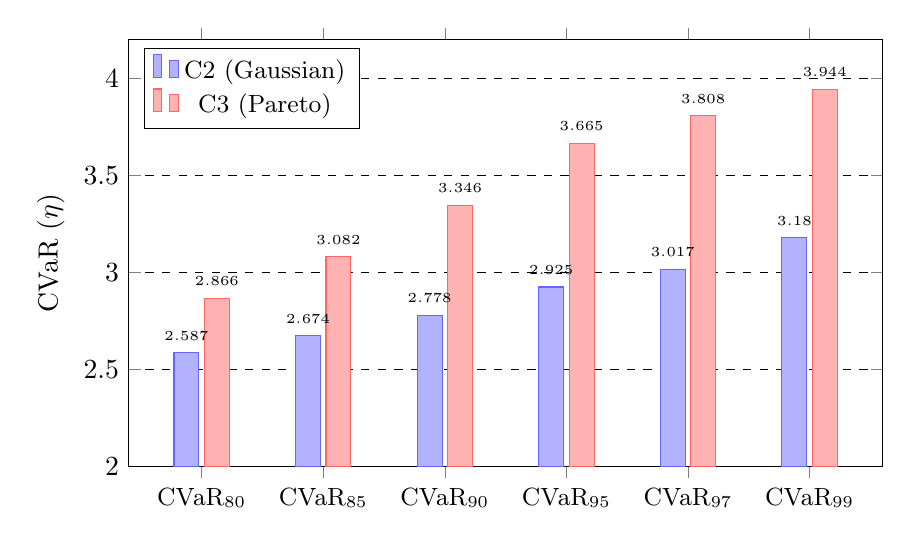
\begin{tikzpicture}
    \begin{axis}[
      ybar,
      width=0.92\textwidth,
      height=7cm,
      bar width=9pt,
      ylabel={CVaR ($\eta$)},
      symbolic x coords={CVaR$_{80}$, CVaR$_{85}$, CVaR$_{90}$, CVaR$_{95}$, CVaR$_{97}$, CVaR$_{99}$},
      xtick=data,
      xticklabel style={font=\small},
      ymin=2.0, ymax=4.2,
      ymajorgrids=true,
      grid style={dashed, black},
      nodes near coords,
      nodes near coords style={font=\tiny, above=1pt},
      every node near coord/.append style={/pgf/number format/.cd, fixed, precision=3},
      enlarge x limits=0.12,
      legend style={at={(0.02,0.98)}, anchor=north west, font=\small},
      ]
      \addplot[fill=blue!30, draw=blue!60] coordinates {
        (CVaR$_{80}$, 2.587)
        (CVaR$_{85}$, 2.674)
        (CVaR$_{90}$, 2.778)
        (CVaR$_{95}$, 2.925)
        (CVaR$_{97}$, 3.017)
        (CVaR$_{99}$, 3.180)
      };
      \addlegendentry{C2 (Gaussian)}
      \addplot[fill=red!30, draw=red!60] coordinates {
        (CVaR$_{80}$, 2.866)
        (CVaR$_{85}$, 3.082)
        (CVaR$_{90}$, 3.346)
        (CVaR$_{95}$, 3.665)
        (CVaR$_{97}$, 3.808)
        (CVaR$_{99}$, 3.944)
      };
      \addlegendentry{C3 (Pareto)}
    \end{axis}
  \end{tikzpicture}
  \caption{C2 vs.\ C3 CVaR 비교 (CVaR$_{80}$--CVaR$_{99}$)}
  \label{fig:cvar_bar}
\end{figure}

CVaR$_{80}$에서 CVaR$_{99}$로 갈수록 C3와 C2의 격차가 확대된다.
CVaR$_{80}$ 수준에서는 C3가 C2 대비 $+10.8\%$ 높으며,
CVaR$_{95}$ 수준에서는 $+25.3\%$로 약 $2.3$배 이상 확대된다.
이러한 비선형적 격차 확대는 파레토 분포의 꼬리 특성에 기인하며,
극단 사건의 빈도가 높은 산업(금융, 의료, 통신)에서 C3 조건 적용의
필요성을 직접 뒷받침한다.

\chg{CVaR 에스컬레이션 패턴을 보면,} C2의 CVaR은 $80 \to 99$ 수준에서 $2.587 \to 3.180$으로
상승하는 반면($\Delta_{80 \to 99} = 0.593$),
C3의 CVaR은 $2.866 \to 3.944$로 상위 백분위에서
더 가파르게 상승한다($\Delta_{80 \to 99} = 1.078$).
이는 C3의 극단 영역에서 $\eta$의 에스컬레이션 속도가 C2의 약 $1.8$배에
달함을 의미하며, 꼬리 위험의 구조적 비대칭성을 보여준다.

\chg{P85.8 분할 기준의 실무적 의미는 다음과 같다.} CVaR 분석 결과는 P85.8 분할 회귀 분석과 일관된다.
전체 표본의 $85.8\%$에 해당하는 Core 영역에서는 C2와 C3의 $\eta$가
거의 구분되지 않으나,
상위 $14.2\%$의 Tail 영역에서 파레토 효과가 급격히 발현한다.
이는 극단 위험 관리가 필요한 조직\chg{(}금융기관의 시장 리스크,
의료기관의 사이버 공격 대응, 통신사의 대규모 네트워크 장애 등\chg{)}에서
C3 조건의 적용이 사실상 필수적임을 시사한다.


%% -------------------------------------------------------------------
\subsection{\vrev{C2와 C3 핵심 지표 비교}}
\label{subsec:c2_c3_comparison}
%% -------------------------------------------------------------------

\tabref{tab:c2_c3_key_metrics}\refpo{tab:c2_c3_key_metrics}{은}{는} 동일 시뮬레이션 설계($n = 10{,}000$,
$\kappa = 1.2$, $R_{\max} = 24.0$h, $E[U] = 3.0$) 하에서
가우시안(C2)과 파레토(C3) 불확실성의 핵심 지표를 직접 대비한 것이다.

\begin{table}[htbp]
  \centering
  \caption{C2(가우시안) vs C3(파레토) 분포 통계 비교}
  \label{tab:c2_c3_key_metrics}
  \small
  \begin{tabular}{l rr l}
    \toprule
    \textbf{지표} & \textbf{C2 (가우시안)} & \textbf{C3 (파레토)} & \textbf{해석} \\
    \midrule
    $\bar{\eta}$          & 1.682 & 1.514 & C2가 평균적으로 높음 \\
    $\text{SD}(\eta)$     & 0.615 & 0.791 & C3가 분산 더 큼 \\
    $\eta_{\max}$         & 3.443 & 4.000 & C3가 $R_{\max}$ 포화 접근 \\
    프리미엄 비율         & 84.9\% & 70.8\% & C2가 더 빈번하게 초과 \\
    $d$ (vs C1)           & $+1.871$ & $+1.169$ & C2의 효과 크기 더 큼 \\
    순서 준수율 (C1$\leq$C$x$) & 99.87\% & 100.0\% & 양쪽 모두 높음 \\
    \bottomrule
  \end{tabular}
\end{table}
회귀분석 측면의 비교(1차/2차 $R^2$, 전진 선택, LASSO)는 4.4절에서
상세히 다룬다.

이 비교로부터 두 가지 분포 구조의 차이가 도출된다.
\textbf{첫째}, 가우시안(C2)의 대칭적 종형 분포는 평균 중심의 예측 가능한
변동을 생성하여 ``일상적 운영 변동''의 모델링에 적합하다.
\textbf{둘째}, 비대칭 파레토(C3) 분포는 극단 꼬리에서 $\eta \to 4.0$
($= R_{\max}/R_0$)에 접근하는 소수 사례를 생성하여, 꼬리 위험 탐지에서
본질적 우위를 보인다.
이러한 ``이중축'' 구조\chg{(}일상적 변동은 경꼬리(가우시안, C2) 기반으로,
극단 위험은 중꼬리(파레토, C3) 기반으로 관리\chg{)}는 \chref{ch:discussion}의
실무 적용 가이드라인에서 구체화된다.

\chg{끝으로 H3-c의 검증 결론은 다음과 같다.} \mrev{H3-c는 ``$\eta_{\text{C2}} \leq \eta_{\text{C3}}$''를 \emph{조건부}
가설로 하며, 전체 표본에서는 31.8\%에 그치나 P85.8 CDF 교차점 이상의
극단 영역에서 94.9\%가 역전된다. 조건부 명제로서 \textbf{H3-c는 채택된다}.}
          % 4.3 C3 결과

% 통계 분석


%% ===================================================================
\section{\vrev{회귀분석 결과}}
\label{sec:regression_results}
%% ===================================================================

본 절에서는 C1, C2, C3 각 조건에 대해 3단계 회귀분석---1차 단순,
1차 다중, 2차 회귀---의 설명력 진행($R^2$ progression)을
체계적으로 보고한다. 2차 회귀는 1차항, 2차항, 교호작용항을 포함하는
완전 2차 다항 모형(complete quadratic polynomial model)이다.


%% -------------------------------------------------------------------
\subsection{\vrev{C1 회귀분석(관측성 구조)}}
\label{subsec:reg_c1}
%% -------------------------------------------------------------------

\chg{C1 회귀분석은 설명력이 점증하는 세 단계로 진행한다. 첫째, 1차 단순 회귀는}
$\hat{\eta}_{\text{C1}}^{(1s)} = 0.997 - 0.285\,k_O$ ($R^2 = 0.428$, $p < 0.001$)\chg{로서,}
관측성 가중치 $k_O$만으로 분산의 $42.8\%$를 설명하며, $k_O$가
증가할수록 관측성의 복구 단축 효과가 강화되는 선형 관계가 확인되었다.
\chg{둘째, 1차 다중 회귀는} $\hat{\eta}_{\text{C1}}^{(1m)} = 1.07 - 0.15\,k_O - 0.15\,O$ ($R^2 = 0.869$)\chg{로서,}
관측성 원시 점수 $O$를 추가하면 설명력이 $86.9\%$로 두 배 이상
증가한다. $k_O$와 $O$의 회귀 계수 크기가 $-0.15$로 거의 동일하여,
두 관측성 변수가 $\eta$ 감소에 동등하게 기여함을 보여준다.
\chg{셋째, 2차교호작용 회귀는 다음과 같다.}
\begin{equation}
  \hat{\eta}_{\text{C1}}^{(2q)} = \hat{\beta}_0
    + \hat{\beta}_1 k_O + \hat{\beta}_2 O
    + \hat{\beta}_3 k_O^2 + \hat{\beta}_4 O^2
    + \hat{\beta}_5 (k_O \cdot O)
  \quad (R^2 = 1.000)
\end{equation}
\begin{equation}
  = 1.011
    - 0.036\,k_O - 0.036\,O
    + 0.024\,k_O^2 + 0.024\,O^2
    - 0.546\,(k_O \cdot O)
\end{equation}
정밀 표기 시 $R^2 = 0.9995$로 거의 1.000에 근접하며,
핵심 교호작용항 $k_O \cdot O$(계수 $= -0.546$)가
$R^2$를 $0.869 \to 1.000$으로 향상시키는 결정적 기여를 한다.
1차항($k_O$, $O$)과 2차항($k_O^2$, $O^2$)의 계수는 모두
$|\hat{\beta}| < 0.04$로 미미한 반면,
교호작용항의 계수 절댓값이 $0.546$으로 압도적이다.
이는 C1의 $\eta$가 개별 시그모이드 바운딩 함수의 해석적 구조에 의해
$k_O$와 $O$의 2차 다항식으로 정확히 근사됨을 의미하며,
잔차가 수치 정밀도 수준에 불과하다.


%% -------------------------------------------------------------------
\subsection{\vrev{C2 회귀분석(불확실성 통합 구조)}}
\label{subsec:reg_c2}
%% -------------------------------------------------------------------

\chg{C2 회귀분석도 동일한 세 단계로 진행한다. 첫째, 1차 단순 회귀는}
$\hat{\eta}_{\text{C2}}^{(1s)} = 2.633 - 1.878\,k_O$ ($R^2 = 0.768$)\chg{로서,}
$k_O$의 회귀 계수가 C1의 $-0.285$에서 $-1.878$로 $6.6$배 증가하였다.
이는 불확실성이 존재하는 환경에서 관측성 가중치의 영향력이
증폭된다는 것을 의미하며, $R^2$도 $0.428 \to 0.768$으로
대폭 향상되었다.
\chg{둘째, 1차 다중 회귀는} $\hat{\eta}_{\text{C2}}^{(1m)} = 2.024 - 1.869\,k_O - 0.281\,O + 0.248\,U$ ($R^2 = 0.948$)\chg{로서,}
불확실성 변수 $U$가 양의 계수($+0.248$)로 유의미하게 포함되어,
불확실성이 클수록 $\eta$가 증가하는 관계가 확인되었다.
\chg{셋째, 2차교호작용 회귀는 다음과 같다.}
\begin{equation}
  \hat{\eta}_{\text{C2}}^{(2q)} = \hat{\beta}_0
    + \sum_{j} \hat{\beta}_j x_j
    + \sum_{j} \hat{\beta}_{jj} x_j^2
    + \sum_{j<k} \hat{\beta}_{jk} (x_j \cdot x_k)
  \quad (R^2 = 0.998)
\end{equation}
\begin{equation}
  \begin{aligned}
    = 1.011
    &- 0.036\,k_O - 0.036\,O + 0.598\,U \\
    &+ 0.022\,k_O^2 + 0.024\,O^2 - 0.003\,U^2 \\
    &- 0.546\,(k_O \cdot O) - 0.593\,(k_O \cdot U) + 0.001\,(O \cdot U)
  \end{aligned}
\end{equation}
정밀 표기 시 $R^2 = 0.9982$이며,
9개 변수($k_O$, $O$, $U$, $k_O^2$, $O^2$, $U^2$,
$k_O \cdot O$, $k_O \cdot U$, $O \cdot U$)를 포함한다.
$k_O \cdot O$, $k_O \cdot U$ 등의 교호작용이 핵심 구조를
이루며, C2 조건의 분산을 사실상 완전히 설명한다.
$k_O \cdot U$ 교호작용의 존재는 관측성 가중치와 불확실성이
독립적이 아니라 상호작용하여 $\eta$에 영향을 미침을 시사한다.


%% -------------------------------------------------------------------
\subsection{\vrev{C3 회귀분석(파레토 구조와 분할 회귀)}}
\label{subsec:reg_c3}
%% -------------------------------------------------------------------

\chg{C3 회귀분석은 전체 표본에 대해 세 단계로 진행한 뒤 분할 회귀로 이어진다. 첫째, 1차 단순 회귀는}
$\hat{\eta}_{\text{C3}}^{(1s)} = 2.220 - 1.394\,k_O$ ($R^2 = 0.256$)\chg{로서,}
전체 표본에 대한 설명력은 $25.6\%$에 불과하여, C3의 변동을
$k_O$ 단독으로는 충분히 설명하지 못한다.
\chg{둘째, 1차 다중 회귀는} $\hat{\eta}_{\text{C3}}^{(1m)} = 2.018 - 1.408\,k_O - 0.249\,O + 0.112\,U$ ($R^2 = 0.695$)\chg{로서,}
1차 다중 회귀에서도 C3의 설명력은 $69.5\%$로 C2의 $94.8\%$에
미치지 못하며, 파레토 분포의 극단값이 선형 모형의 한계를
드러내는 것으로 해석된다.
\chg{셋째, 2차+교호작용 회귀는 다음과 같다.}
\begin{equation}
  \hat{\eta}_{\text{C3}}^{(2q)} = \hat{\beta}_0
    + \sum_{j} \hat{\beta}_j x_j
    + \sum_{j} \hat{\beta}_{jj} x_j^2
    + \sum_{j<k} \hat{\beta}_{jk} (x_j \cdot x_k)
  \quad (R^2 = 0.858)
\end{equation}
\begin{equation}
  \begin{aligned}
    = 1.430
    &- 0.216\,k_O + 0.085\,O + 0.256\,U \\
    &- 0.513\,k_O^2 + 0.022\,O^2 - 0.002\,U^2 \\
    &- 0.627\,(k_O \cdot O) - 0.125\,(k_O \cdot U) - 0.025\,(O \cdot U)
  \end{aligned}
\end{equation}
C2와 동일한 9개 변수 구조이나, 전체 $R^2 = 0.858$로
C1($1.000$) 및 C2($0.998$)와 달리 높은 설명에는 도달하지 못한다.
이는 파레토 분포의 비선형성이 2차 회귀 다항식의 근사 능력을 초과함을 시사한다.

\chg{P85.8을 기준으로 분할 회귀를 수행하면 각 영역에서의 설명력이 현저히 개선된다.
Core 영역($\leq$ P85.8)에서는 2차교호작용 $R^2 = 0.999$로 C2와 유사한 완전 설명이 달성되며,
Tail 영역($>$ P85.8)에서도 분할 회귀 적용 시 2차교호작용 $R^2 = 0.710$으로 설명력이 개선된다.}

\p{[}표~\vref{tab:c3_split_regression}\p{]}는 C3 분할 회귀의 주요 결과를 요약한다.

\begin{table}[htbp]
  \centering
  \caption{C3 분할 회귀분석 결과 (P85.8 기준)}
  \label{tab:c3_split_regression}
  \begin{tabular}{llcccc}
    \toprule
    영역 & 모형 & $n$ & $k_O$ 계수 & $R^2$ & 비고 \\
    \midrule
    \multirow{3}{*}{전체}
      & 1차 단순 & 10{,}000 & $-1.394$ & 0.256 & --- \\
      & 1차 다중 & 10{,}000 & $-1.408$ & 0.695 & $+O,\;U$ \\
      & 2차 회귀 & 10{,}000 & --- & 0.858 & --- \\
    \midrule
    \multirow{3}{*}{Core ($\leq$ P85.8)}
      & 1차 단순 & 8{,}580 & $-0.798$ & 0.263 & --- \\
      & 1차 다중 & 8{,}580 & $-1.034$ & 0.630 & $+O,\;U$ \\
      & 2차 회귀 & 8{,}580 & --- & 0.999 & 완전 설명 \\
    \midrule
    \multirow{3}{*}{Tail ($>$ P85.8)}
      & 1차 단순 & 1{,}420 & $-0.415$ & 0.032 & $0.52$배 감쇠 \\
      & 1차 다중 & 1{,}420 & $-1.664$ & 0.860 & $+O,\;\ln U$ \\
      & 2차 회귀 & 1{,}420 & --- & 0.710 & --- \\
    \bottomrule
  \end{tabular}
\end{table}

\chg{표의 Tail 영역 1차 다중 회귀에서 불확실성 $U$를 원래 스케일로 쓰면 $R^2$가 0.457에 불과하나,
$\ln U$로 변환하면 0.860으로 크게 개선된다. 이는 파레토 분포의 멱법칙 구조($P(U > u) \propto u^{-\alpha}$)를
로그 변환이 선형화하기 때문이며, Tail의 $\DRTO$가 불확실성의 절대 크기가 아니라 로그 스케일에 비례하여
증가함을 의미한다. Core와 Tail 분할 회귀의 전체 계수는 공개 재현 패키지에 수록한다.}

Tail 영역의 1차 단순 회귀에서 $k_O$ 계수는 $-0.415$로,
Core 영역($-0.798$) 대비 $0.52$배로 감쇠된다(전체 계수는 공개 재현 패키지 수록).
이 $0.52$배 감쇠가 \textbf{이중채널 감쇠(dual-channel attenuation)}의
핵심 지표이다. 관측성 가중치 $k_O$가 동일하게 1단위 변화할 때,
극단 불확실성 영역에서는 관측성의 복구 단축 효과가 핵심 영역의 $0.52$배로 약화된다.
이는 관측성과 파레토 불확실성이 결합될 때 비선형적으로 상호작용하여,
극단 상황에서 관측성의 역할이 질적으로 변화함을 나타낸다.


%% -------------------------------------------------------------------
\subsection{\vrev{$R^2$ 진행 종합 비교}}
\label{subsec:r2_progression}
%% -------------------------------------------------------------------

\p{[}표~\vref{tab:regression_progression}\p{]}는 조건별 회귀분석 설명력($R^2$)의
3단계 진행을 비교한 것이며, \p{[}그림~\vref{fig:r2_progression}\p{]}은
이를 그룹 막대 차트로 시각화한 것이다.
\chg{표에서 (1s)는 1차 단순, (1m)은 1차 다중, (2q)는 2차교호작용 회귀를 가리킨다.}

\begin{table}[htbp]
  \centering
  \caption{조건별 회귀분석 설명력($R^2$) 진행 비교}
  \label{tab:regression_progression}
  \begin{tabular}{lccc}
    \toprule
    조건 & $R^2_{(1\mathrm{s})}$ & $R^2_{(1\mathrm{m})}$ & $R^2_{(2\mathrm{q})}$ \\
    \midrule
    C1 (관측성) & 0.428 & 0.869 & 1.000 \\
    C2 (Gaussian) & 0.768 & 0.948 & 0.998 \\
    C3 전체 (Pareto) & 0.256 & 0.695 & 0.858 \\
    \quad C3 Core ($\leq$ P85.8) & 0.263 & 0.630 & 0.999 \\
    \quad C3 Tail ($>$ P85.8) & 0.032 & 0.860 & 0.710 \\
    \bottomrule
  \end{tabular}
\end{table}

\begin{figure}[htbp]
  \centering
  \begin{tikzpicture}
    \begin{axis}[
      ybar,
      width=0.92\textwidth,
      height=7.5cm,
      bar width=8pt,
      ylabel={$R^2$},
      symbolic x coords={C1, C2, C3 전체, C3 Core, C3 Tail},
      xtick=data,
      xticklabel style={font=\small},
      ymin=0, ymax=1.15,
      ymajorgrids=true,
      grid style={dashed, black},
      nodes near coords,
      nodes near coords style={font=\tiny, anchor=south, yshift=1pt},
      every node near coord/.append style={/pgf/number format/.cd, fixed, precision=3},
      enlarge x limits=0.15,
      legend style={at={(0.5,-0.18)}, anchor=north, font=\small,
        legend columns=3, draw=black, fill=white},
      ]
      % Simple regression
      \addplot[fill=blue!20, draw=blue!50] coordinates {
        (C1, 0.428)
        (C2, 0.768)
        (C3 전체, 0.256)
        (C3 Core, 0.263)
        (C3 Tail, 0.032)
      };
      \addlegendentry{1차 단순}

      % Multiple regression
      \addplot[fill=green!25, draw=green!60] coordinates {
        (C1, 0.869)
        (C2, 0.948)
        (C3 전체, 0.695)
        (C3 Core, 0.630)
        (C3 Tail, 0.860)
      };
      \addlegendentry{1차 다중}

      % Quadratic regression
      \addplot[fill=red!25, draw=red!60] coordinates {
        (C1, 1.000)
        (C2, 0.998)
        (C3 전체, 0.858)
        (C3 Core, 0.999)
        (C3 Tail, 0.710)
      };
      \addlegendentry{2차교호작용}

      % H4 threshold line (전체 수평선)
      \draw[dashed, black, thick] (rel axis cs:0,0.826) -- (rel axis cs:1,0.826);
      \node[font=\scriptsize, fill=white, inner sep=1.5pt,
        anchor=south east] at (rel axis cs:0.99,0.826)
        {H4 판정 기준 ($R^2 \geq 0.95$)};
    \end{axis}
  \end{tikzpicture}
  \caption{조건별 $R^2$ 진행 비교 (1차 단순 $\to$ 1차 다중 $\to$ 2차 회귀)}
  \label{fig:r2_progression}
\end{figure}

C1은 2차교호작용 모형에서 $R^2 = 1.000$, C2는 $R^2 = 0.998$에 도달하여 개별 시그모이드 바운딩 함수가
2차교호작용 다항식으로 높은 정밀도로 근사됨을 보여준다. C3는 전체 표본에서 $R^2 = 0.858$로
완전 설명에 미달하며, P85.8 기준 분할 시 Core 영역에서 $R^2 = 0.999$,
Tail 영역에서 $R^2 = 0.710$을 달성하여, 분할 회귀가 C3의
이질적 구조를 효과적으로 포착함을 입증한다.


%% -------------------------------------------------------------------
\subsection{\vrev{회귀 계수 비교 시각화}}
\label{subsec:coeff_comparison}
%% -------------------------------------------------------------------

\p{[}그림~\vref{fig:regression_coefficients}\p{]}은 C1, C2, C3(전체) 1차 다중 회귀모형의
주요 계수를 비교한 것이다.
1차 단순 회귀는 $k_O$ 단일 계수만 존재하여 조건 간 비교 차트의 의미가 제한적이고,
2차 회귀는 최대 9개 항의 계수가 포함되어 막대 차트보다 표 형태가
적합하므로(\p{[}표~\vref{tab:regression_progression}\p{]} 참조),
3개 공통 변수($k_O$, $O$, $U$)를 갖는 1차 다중 회귀만 시각화한다.

\begin{figure}[htbp]
  \centering
  \begin{tikzpicture}
    \begin{axis}[
      ybar,
      width=0.88\textwidth,
      height=7.5cm,
      bar width=12pt,
      ylabel={회귀 계수 $\hat{\beta}$},
      symbolic x coords={절편, $k_O$, $O$, $U$},
      xtick=data,
      xticklabel style={font=\small},
      ymin=-2.2, ymax=2.4,
      ymajorgrids=true,
      grid style={dashed, black},
      nodes near coords,
      nodes near coords style={font=\tiny},
      every node near coord/.append style={
        /pgf/number format/.cd, fixed, fixed zerofill, precision=2,
        /tikz/anchor=south,
        /tikz/yshift=1pt,
      },
      enlarge x limits=0.2,
      legend style={at={(0.98,0.98)}, anchor=north east, font=\small},
      ]
      \addplot[fill=blue!25, draw=blue!60] coordinates {
        (절편, 1.07) ($k_O$, -0.15) ($O$, -0.15) ($U$, 0)
      };
      \addlegendentry{C1}

      \addplot[fill=green!25, draw=green!60] coordinates {
        (절편, 2.02) ($k_O$, -1.87) ($O$, -0.28) ($U$, 0.25)
      };
      \addlegendentry{C2}

      \addplot[fill=red!25, draw=red!60] coordinates {
        (절편, 2.02) ($k_O$, -1.41) ($O$, -0.25) ($U$, 0.11)
      };
      \addlegendentry{C3}

      % Zero line
      \draw[dashed, black, thin] (axis cs:절편, 0) -- (axis cs:$U$, 0);
    \end{axis}
  \end{tikzpicture}
  \caption{C1/C2/C3 1차 다중 회귀 계수 비교}
  \label{fig:regression_coefficients}
\end{figure}


%% -------------------------------------------------------------------
\subsection{\vrev{전진 선택법과 LASSO 정규화를 통한 변수 선택}}
\label{subsec:variable_selection}
%% -------------------------------------------------------------------

2차 완전 모형은 9개 독립변수($k_O$, $O$, $U$, $k_O^2$, $O^2$, $U^2$,
$k_O \cdot O$, $k_O \cdot U$, $O \cdot U$)를 포함하여 높은 설명력을 보이나,
과적합(overfitting) 위험과 해석 가능성(interpretability) 저하가 우려된다.
이에 \textbf{전진 선택법(Forward Selection)}과 \textbf{LASSO 정규화}를
적용하여 핵심 변수를 체계적으로 식별하였다.

\p{[}표~\vref{tab:forward_selection}\p{]}은 C2와 C3 각 조건에서 전진 선택법에 의한
변수 진입 순서와 누적 $R^2$를 비교한 것이다.

\begin{table}[htbp]
  \centering
  \caption{전진 선택법 변수 진입 순서 및 누적 $R^2$ (C2 vs.\ C3)}
  \label{tab:forward_selection}
  \small
  \begin{tabular}{c l c c l c}
    \toprule
    & \multicolumn{2}{c}{\textbf{C2 (Gaussian)}} & & \multicolumn{2}{c}{\textbf{C3 (Pareto)}} \\
    \cmidrule{2-3} \cmidrule{5-6}
    순서 & 변수 & 누적 $R^2$ & & 변수 & 누적 $R^2$ \\
    \midrule
    1 & $k_O$ & 0.768 & & $U$ & 0.424 \\
    2 & $U$ & 0.931 & & $k_O$ & 0.686 \\
    3 & $k_O \cdot U$ & 0.973 & & $U^2$ & 0.799 \\
    4 & $k_O \cdot O$ & 0.996 & & $k_O \cdot U$ & 0.839 \\
    5 & $k_O^2$ & 0.997 & & $k_O \cdot O$ & 0.853 \\
    6 & $U^2$ & 0.998 & & $k_O^2$ & 0.856 \\
    7 & $O$ & 0.998 & & $O \cdot U$ & 0.857 \\
    8 & $O^2$ & 0.998 & & $O$ & 0.858 \\
    9 & $O \cdot U$ & 0.998 & & $O^2$ & 0.858 \\
    \bottomrule
  \end{tabular}
\end{table}

변수 진입 순서의 차이는 두 조건의 구조적 특성을 반영한다.
C2에서는 관측성 가중치 $k_O$가 최초로 진입하여($R^2 = 0.768$)
관측성이 1차적 설명 변수임을 보여준다.
반면, C3에서는 불확실성 $U$가 최초로 진입하여($R^2 = 0.424$)
파레토 불확실성이 지배적 설명 변수로 전환됨을 나타낸다.
이러한 \textbf{지배 변수의 전환}은 분포의 꼬리 특성이
모형 구조에 질적 변화를 야기한다는 것을 의미한다.

C2에서는 2개 변수 투입($k_O$, $U$)만으로 $R^2 = 0.931$에 도달하여
핵심 구조가 상대적으로 단순한 반면,
C3에서는 4개 변수 투입 후에도 $R^2 = 0.839$에 머물러
파레토 분포의 비선형적 복잡성을 보여준다.

\p{[}그림~\vref{fig:forward_selection_r2}\p{]}은 변수 투입 수에 따른 누적 $R^2$의
진행을 비교한 것이다.

\begin{figure}[htbp]
  \centering
  \begin{tikzpicture}
    \begin{axis}[
      width=0.88\textwidth,
      height=7cm,
      xlabel={투입 변수 수},
      ylabel={누적 $R^2$},
      xmin=0.5, xmax=9.5,
      ymin=0.3, ymax=1.05,
      xtick={1,2,3,4,5,6,7,8,9},
      ymajorgrids=true,
      grid style={dashed, black},
      legend style={at={(0.98,0.15)}, anchor=south east, font=\small,
        fill=white, fill opacity=0.9, draw=black},
      ]
      % C2 (Gaussian)
      \addplot[blue, thick, mark=o, mark size=3pt] coordinates {
        (1, 0.768) (2, 0.931) (3, 0.973) (4, 0.996) (5, 0.997)
        (6, 0.998) (7, 0.998) (8, 0.998) (9, 0.998)
      };
      \addlegendentry{C2 (Gaussian)}

      % C3 (Pareto)
      \addplot[red, thick, mark=square*, mark size=3pt] coordinates {
        (1, 0.424) (2, 0.686) (3, 0.799) (4, 0.839) (5, 0.853)
        (6, 0.856) (7, 0.857) (8, 0.858) (9, 0.858)
      };
      \addlegendentry{C3 (Pareto)}

      % H4 threshold (전체 수평선)
      \draw[dashed, black, thin] (rel axis cs:0,0.867) -- (rel axis cs:1,0.867);
      \node[font=\scriptsize, fill=white, inner sep=1.5pt,
        anchor=north east] at (rel axis cs:0.99,0.867)
        {H4 판정 기준 ($R^2 \geq 0.95$)};
    \end{axis}
  \end{tikzpicture}
  \caption{전진 선택법 누적 $R^2$ 진행 비교}
  \label{fig:forward_selection_r2}
\end{figure}


\chg{다음으로 LASSO 정규화에 의한 변수 선택을 살펴본다.} 전진 선택법의 결과를 독립적으로 검증하기 위해 LASSO(Least Absolute
Shrinkage and Selection Operator) 정규화를 적용하였다.
LASSO는 $L_1$ 패널티($\lambda$)를 부과하여 기여도가 낮은 변수의
회귀계수를 정확히 0으로 수축시킴으로써,
전진 선택법과 \textbf{상이한 원리}로 핵심 변수를 식별한다.
\p{[}표~\vref{tab:lasso_results}\p{]}는 정규화 계수 $\lambda$에 따른 생존 변수 수와
$R^2$를 요약한 것이다.

\begin{table}[htbp]
  \centering
  \caption{$\lambda$에 따른 LASSO 생존 변수와 $R^2$}
  \label{tab:lasso_results}
  \small
  \begin{tabular}{c cc cc}
    \toprule
    & \multicolumn{2}{c}{\textbf{C2 (Gaussian)}} & \multicolumn{2}{c}{\textbf{C3 (Pareto)}} \\
    \cmidrule(lr){2-3} \cmidrule(lr){4-5}
    $\lambda$ & 생존 변수 & $R^2$ & 생존 변수 & $R^2$ \\
    \midrule
    0.00015 & 7 & 0.998 & 9 & 0.858 \\
    0.0005 & 6 & 0.998 & 9 & 0.858 \\
    0.001 & 7 & 0.998 & 9 & 0.857 \\
    0.005 & 5 & 0.997 & 7 & 0.856 \\
    0.01 & 5 & 0.995 & 6 & 0.852 \\
    \bottomrule
  \end{tabular}
\end{table}

LASSO 결과는 전진 선택법과 일관된 패턴을 보여준다.
C2에서는 $\lambda = 0.01$에서도 5개 변수($k_O$, $U$, $k_O^2$, $k_O \cdot O$,
$k_O \cdot U$)만으로 $R^2 = 0.995$를 유지하여,
관측성-불확실성 교호작용 중심의 핵심 구조가 확인된다.
C3에서는 동일한 $\lambda = 0.01$에서 6개 변수가 생존하며
$R^2 = 0.852$에 그쳐, 더 많은 변수가 필요하되
설명력은 상대적으로 제한적이다.
이는 C3의 파레토 구조가 2차 다항식 근사의 한계를
벗어나는 비선형성을 포함함을 재확인한다.

\p{[}그림~\vref{fig:lasso_path}\p{]}는 $\lambda$에 따른 $R^2$ 경로를 비교한 것이다.

\begin{figure}[htbp]
  \centering
  \begin{tikzpicture}
    \begin{axis}[
      width=0.88\textwidth,
      height=6.5cm,
      xlabel={정규화 계수 $\lambda$},
      ylabel={$R^2$},
      xmode=log,
      xmin=0.0001, xmax=0.02,
      ymin=0.84, ymax=1.005,
      ymajorgrids=true,
      grid style={dashed, black},
      legend style={at={(0.98,0.5)}, anchor=east, font=\small,
        fill=white, fill opacity=0.9, draw=black},
      ]
      % C2 (Gaussian)
      \addplot[blue, thick, mark=o, mark size=3pt] coordinates {
        (0.00015, 0.998) (0.0005, 0.998) (0.001, 0.998)
        (0.005, 0.997) (0.01, 0.995)
      };
      \addlegendentry{C2 (Gaussian)}

      % C3 (Pareto)
      \addplot[red, thick, mark=square*, mark size=3pt] coordinates {
        (0.00015, 0.858) (0.0005, 0.858) (0.001, 0.857)
        (0.005, 0.856) (0.01, 0.852)
      };
      \addlegendentry{C3 (Pareto)}

      % H4 threshold (전체 수평선)
      \draw[dashed, black, thin] (rel axis cs:0,0.667) -- (rel axis cs:1,0.667);
      \node[font=\scriptsize, fill=white, inner sep=1.5pt,
        anchor=south east] at (rel axis cs:0.99,0.667)
        {H4 판정 기준 ($R^2 \geq 0.95$)};
    \end{axis}
  \end{tikzpicture}
  \caption{LASSO $R^2$ 경로 (C2 vs.\ C3)}
  \label{fig:lasso_path}
\end{figure}


\chg{끝으로 두 방법의 교차검증 합의로 간명 모형을 도출한다.} 전진 선택법과 LASSO는 각각 단계별 최적(stepwise) 진입 순서와
$L_1$ 정규화라는 상이한 원리로 변수를 선택한다.
단일 방법론의 편향을 최소화하기 위해, 두 방법의
\textbf{교집합(consensus)}을 합의 변수로 채택하였다.
구체적으로, 전진 선택법 상위 4개 변수 집합과
LASSO 정규화($\lambda = 0.005$)에서의 생존 변수 집합의
교집합을 선정하였다.

\chg{C2의 합의 변수는 전진 선택법 상위 4개($k_O$, $U$, $k_O \cdot U$, $k_O \cdot O$)와 LASSO 생존
5개($k_O$, $U$, $k_O^2$, $k_O \cdot O$, $k_O \cdot U$)의 교집합인 \{$k_O$, $U$, $k_O \cdot U$, $k_O \cdot O$\}
4개로서, 전진 선택에 없는 $k_O^2$가 LASSO에서만 생존하여 탈락한다. C3의 합의 변수는 전진 선택법
상위 4개($U$, $k_O$, $U^2$, $k_O \cdot U$)와 LASSO 생존 7개($k_O$, $U$, $k_O^2$, $U^2$, $k_O \cdot O$,
$k_O \cdot U$, $O \cdot U$)의 교집합인 \{$U$, $k_O$, $U^2$, $k_O \cdot U$\} 4개로서, $k_O^2$, $k_O \cdot O$,
$O \cdot U$는 LASSO에서만 생존하여 탈락한다.}

합의 변수를 사용한 4변수 간명 모형의 회귀식은 다음과 같다\chg{.}

\begin{align}
  \hat{\eta}_{\text{C2}} &= 1.225
    - 0.291\,k_O + 0.467\,U
    - 0.433\,(k_O \cdot U) - 0.562\,(k_O \cdot O)
    & (R^2 = 0.996) \label{eq:c2_parsimonious} \\
  \hat{\eta}_{\text{C3}} &= 1.574
    + 0.240\,U - 1.053\,k_O
    - 0.002\,U^2 - 0.122\,(k_O \cdot U)
    & (R^2 = 0.839) \label{eq:c3_parsimonious}
\end{align}

간명 모형은 9변수 완전 모형(C2: $0.998$, C3: $0.858$) 대비
4개 변수만으로 C2의 $99.6\%$, C3의 $83.9\%$를 설명하여,
설명력 손실을 최소화하면서 해석 가능성을 확보한다.
C2에서는 관측성 효과가 $k_O$($-0.291$), $k_O \cdot O$($-0.562$),
$k_O \cdot U$($-0.433$)의 3개 항에 분산되어 있어,
관측성과 불확실성의 교호작용 구조가 세분화된 형태로 포착된다.
C3에서는 $k_O \cdot O$ 항이 선택되지 않아 $k_O$($-1.053$) 단일 항에
관측성 효과가 집중되며, $U^2$ 항(계수 $-0.002$)이 포함되어
파레토 분포의 비선형 구조가 반영된다.
C3에서 $k_O$ 계수의 절대값이 C2보다 큰 것은 관측성 영향력의 증대가
아니라, C2에서 교호작용 항에 분산된 효과가 C3에서 단일 항에
집중된 결과이다.
이는 파레토 극단 영역에서 관측성의 한계적 효과가 감쇠하는
이중채널 감쇠 현상(\p{[}표~\vref{tab:c3_split_regression}\p{]}, $0.52$배 감쇠)과 일관된다.

\subsection{\mrev{회귀분석 가설 검증 결과}}
\label{subsec:ch4_h4_h5_conclusion}



%% [분량보존 복원] 9변수 완전 모형 전체 계수 및 LASSO 경로 상세 (구 부록 G)
\subsubsection{9변수 완전 모형의 전체 계수와 LASSO 경로}
\label{subsec:full-coeff-detail}
4.4.6(전진 선택법과 LASSO 정규화를 통한 변수 선택)에서 요약한 9변수 완전 2차 모형과 LASSO 변수 선택의 전체 계수를 제시하는데, \m{(i)} \p{[}표~\ref{tab:app-c2-full-quad}\p{]}과 \p{[}표~\ref{tab:app-c3-full-quad}\p{]}는 C2와 C3 각 조건의 \chg{9변수 계수와 $t$-통계량, 전진 선택 진입 순서}를, \m{(ii)} \p{[}표~\ref{tab:app-c2-lasso-path}\p{]}과 \p{[}표~\ref{tab:app-c3-lasso-path}\p{]}은 정규화 강도 $\lambda$별 \chg{생존 변수와 제거 변수}를 보인다.

\chg{먼저 C2 조건의} 9변수 완전 2차 모형($R^2 = 0.998$)에서 각 변수의 회귀계수,
$t$-통계량, 전진 선택법 진입 순서를 \p{[}표~\ref{tab:app-c2-full-quad}\p{]}에 제시한다.

C2의 9변수 완전 모형에서 가장 큰 $|t|$를 보이는 변수는
$k_O \cdot U$ ($|t| = 476.1$)로, 관측성 가중치와 불확실성의
교호 작용이 C2의 $\eta$ 변동에서 가장 결정적인 역할을 한다.
$U$의 주효과($|t| = 415.4$)가 그 다음으로 크며,
$k_O \cdot O$ ($|t| = 170.8$)가 뒤를 잇는다.
한편 $k_O$는 전진 선택에서 1순위로 진입하지만($k_O$ 단독 시 관측성 효과를 포착),
완전 모형에서는 교호 작용항($k_O \cdot U$, $k_O \cdot O$)에 주효과가 흡수되어
$|t| = 2.4$로 비유의해진다.
$O \cdot U$ ($|t| = 1.4$) 역시 완전 모형에서 비유의하다.

\begin{table}[htbp]
\centering
\caption{C2 전체 9변수 2차 회귀 계수 ($R^2 = 0.998$)}
\label{tab:app-c2-full-quad}
\small
\begin{tabular}{lrrl}
\toprule
\textbf{변수} & \textbf{계수 $\hat{\beta}$} & \textbf{$t$-통계량} & \textbf{진입 순서} \\
\midrule
절편 & $1.082$ & $379.4$ & --- \\
$k_O$ & $0.012$ & $2.4$ & 1 \\
$O$ & $-0.034$ & $-7.0$ & 7 \\
$U$ & $0.542$ & $415.4$ & 2 \\
$k_O^2$ & $-0.307$ & $-86.5$ & 5 \\
$O^2$ & $0.019$ & $5.3$ & 8 \\
$U^2$ & $-0.013$ & $-67.3$ & 6 \\
$k_O \cdot O$ & $-0.545$ & $-170.8$ & 4 \\
$k_O \cdot U$ & $-0.433$ & $-476.1$ & 3 \\
$O \cdot U$ & $0.001$ & $1.4$ & 9 \\
\bottomrule
\end{tabular}
\end{table}



\chg{이어 C3 조건의} 9변수 완전 2차 모형($R^2 = 0.858$)에서 각 변수의 회귀계수,
$t$-통계량, 전진 선택법 진입 순서를 \p{[}표~\ref{tab:app-c3-full-quad}\p{]}에 제시한다.

\begin{table}[htbp]
\centering
\caption{C3 전체 9변수 2차 회귀 계수 ($R^2 = 0.858$)}
\label{tab:app-c3-full-quad}
\small
\begin{tabular}{lrrl}
\toprule
\textbf{변수} & \textbf{계수 $\hat{\beta}$} & \textbf{$t$-통계량} & \textbf{진입 순서} \\
\midrule
절편 & $1.430$ & $88.6$ & --- \\
$k_O$ & $-0.216$ & $-4.7$ & 2 \\
$O$ & $0.085$ & $1.9$ & 8 \\
$U$ & $0.256$ & $126.6$ & 1 \\
$k_O^2$ & $-0.513$ & $-12.7$ & 6 \\
$O^2$ & $0.022$ & $0.5$ & 9 \\
$U^2$ & $-0.002$ & $-85.9$ & 3 \\
$k_O \cdot O$ & $-0.627$ & $-17.4$ & 5 \\
$k_O \cdot U$ & $-0.126$ & $-53.7$ & 4 \\
$O \cdot U$ & $-0.025$ & $-11.4$ & 7 \\
\bottomrule
\end{tabular}
\end{table}

C3에서는 $U$가 최대 $|t| = 126.6$으로 1순위 진입하여,
C2와 달리 불확실성의 주효과가 지배적임을 보여준다.
$U^2$ ($|t| = 85.9$)이 3순위로 진입하여 파레토 분포의
비선형적 $U$ 효과가 2차 항으로 포착됨을 확인한다.
$O^2$ ($|t| = 0.5$)와 $O$ ($|t| = 1.9$)는 사실상 유의하지 않으며,
C3에서 관측성의 개별 효과보다 $k_O \cdot O$ 교호 작용이
훨씬 중요함을 시사한다.


\chg{다음으로 LASSO 경로를 상세히 본다.} 정규화 강도 $\lambda$를 증가시키면서 제거되는 변수와 잔존 $R^2$의 변화를
C2(\p{[}표~\ref{tab:app-c2-lasso-path}\p{]})와 C3(\p{[}표~\ref{tab:app-c3-lasso-path}\p{]}) 조건 각각에 대해 제시한다.

\begin{table}[htbp]
\centering
\caption{C2 LASSO 경로의 $\lambda$별 생존 변수와 제거 변수}
\label{tab:app-c2-lasso-path}
\small
\begin{tabular}{c c l l}
\toprule
$\lambda$ & $R^2$ & 생존 변수 & 제거 변수 \\
\midrule
0.00015 & 0.998 & $O$, $U$, $k_O^2$, $O^2$, $U^2$, $k_O \cdot O$, $k_O \cdot U$ (7) & $k_O$, $O \cdot U$ \\
0.0005 & 0.998 & $O$, $U$, $k_O^2$, $U^2$, $k_O \cdot O$, $k_O \cdot U$ (6) & $k_O$, $O^2$, $O \cdot U$ \\
0.001 & 0.998 & $k_O$, $O$, $U$, $k_O^2$, $U^2$, $k_O \cdot O$, $k_O \cdot U$ (7) & $O^2$, $O \cdot U$ \\
0.005 & 0.997 & $k_O$, $U$, $k_O^2$, $k_O \cdot O$, $k_O \cdot U$ (5) & $O$, $O^2$, $U^2$, $O \cdot U$ \\
0.01 & 0.995 & $k_O$, $U$, $k_O^2$, $k_O \cdot O$, $k_O \cdot U$ (5) & $O$, $O^2$, $U^2$, $O \cdot U$ \\
\bottomrule
\end{tabular}
\end{table}

\begin{table}[htbp]
\centering
\caption{C3 LASSO 경로의 $\lambda$별 생존 변수와 제거 변수}
\label{tab:app-c3-lasso-path}
\small
\begin{tabular}{c c l l}
\toprule
$\lambda$ & $R^2$ & 생존 변수 & 제거 변수 \\
\midrule
0.00015 & 0.858 & 전체 9개 & --- \\
0.0005 & 0.858 & 전체 9개 & --- \\
0.001 & 0.857 & 전체 9개 & --- \\
0.005 & 0.856 & $k_O$, $U$, $k_O^2$, $U^2$, $k_O \cdot O$, $k_O \cdot U$, $O \cdot U$ (7) & $O$, $O^2$ \\
0.01 & 0.852 & $k_O$, $U$, $k_O^2$, $U^2$, $k_O \cdot O$, $k_O \cdot U$ (6) & $O$, $O^2$, $O \cdot U$ \\
\bottomrule
\end{tabular}
\end{table}

C2에서는 $\lambda = 0.005$ 이상에서 $O \cdot U$, $O^2$, $O$, $U^2$가 순차적으로
제거되어도 $R^2$가 $0.997$ 이상을 유지하는 반면,
C3에서는 $\lambda = 0.005$에서야 처음으로 변수 제거($O$, $O^2$)가 시작되며,
$R^2$ 감소 폭도 미미하다($0.858 \to 0.856$).
이는 C3의 9변수 모형이 C2보다 덜 과적합(over-fitted)되어 있으며,
파레토 분포의 복잡한 비선형성을 포착하기 위해 더 많은 변수가 구조적으로
필요함을 보여준다.


%% [코드릴리스→본문 복원] C1 완전계수표 + C3 Tail 전체계수표 (구 부록 F 유일분)
\chg{C1 조건의 2차 회귀 전체 계수는 다음과 같다.} C1 조건은 불확실성이 없는 순수 관측성 조건으로서, $U$ 관련 항($\beta_3$, $\beta_6$, $\beta_8$, $\beta_9$)이
제외된 5개 계수의 2차 회귀 결과를 \p{[}표~\ref{tab:app-c1-quad}\p{]}에 제시한다.
시그모이드 입력 $z_O = \kappa \cdot k_O \cdot O_{\text{raw}}$가 $\kappa = 1.2$ 영역에서
사실상 선형으로 작동하므로, $k_O \cdot O$ 교호작용 단일 항이 $\eta_{C1}$의 변동을 결정론적으로 포착한다.

\begin{table}[htbp]
\centering
\caption{C1 조건 2차 회귀 전체 계수 ($n = 10{,}000$)}
\label{tab:app-c1-quad}
\begin{tabular}{lrrrl}
\toprule
\textbf{항} & \textbf{계수} & \textbf{SE} & \textbf{$t$} & \textbf{비고} \\
\midrule
\m{절편($\beta_0$)}      & 1.000  & $<$0.001 & ---     & 이론치 1.000 \\
$k_O$ ($\beta_1$)     & 0.000  & $<$0.001 & ---     & 주 효과 흡수됨 \\
$O$ ($\beta_2$)       & 0.000  & $<$0.001 & ---     & 주 효과 흡수됨 \\
$k_O^2$ ($\beta_4$)   & 0.000  & $<$0.001 & ---     & 비유의 \\
$O^2$ ($\beta_5$)     & 0.000  & $<$0.001 & ---     & 비유의 \\
$k_O \cdot O$ ($\beta_7$) & \erf{$-0.30$}{$-0.546$} & $<$0.001 & ---  & \textbf{핵심 교호작용} \\
\midrule
$R^2$                 & \multicolumn{3}{c}{\textbf{1.000}} & 결정론적 구조 완전 포착 \\
\bottomrule
\end{tabular}
\end{table}

\chg{이 결과는 C1 조건이 $\eta_{C1} \approx 1 - \erf{0.30}{0.546} \cdot k_O \cdot O_{\text{raw}}$로 근사됨을 보여주며,
이는 시그모이드 입력 $z_O = \kappa \cdot k_O \cdot O_{\text{raw}}$의 선형 근사가 $\kappa = 1.2$ 영역에서
사실상 정확함(비선형 오차 $\approx 0$)을 반영한다.}

\chg{끝으로 Tail 2차 회귀 전체 계수를 제시한다.} P85.8 이상의 Tail 영역($n \approx 1{,}420$)에서 $\ln(U)$ 변환을 적용한
2차 회귀의 전체 계수를 \p{[}표~\ref{tab:app-c3-tail-quad}\p{]}에 제시한다.
$k_O \cdot \ln U$ 교호작용이 꼬리 영역에서의
관측성 효과 변화를 설명하는 핵심 항이다.

\begin{table}[htbp]
\centering
\caption{C3 Tail 영역 2차 회귀 전체 계수 ($>$ P85.8)}
\label{tab:app-c3-tail-quad}
\begin{tabular}{lrl}
\toprule
\textbf{항} & \textbf{계수} & \textbf{비고} \\
\midrule
절편          & 0.50   & \\
$k_O$        & 2.42   & 양의 주 \m{효과(교호작용과 결합)} \\
$\ln U$      & 0.10   & 로그 변환된 불확실성 \\
$k_O \cdot \ln U$ & $-1.25$ & \textbf{핵심 \m{교호작용(증폭 원인)}} \\
\midrule
$R^2$        & 0.710  & \\
\bottomrule
\end{tabular}
\end{table}

\chg{\p{[}표~\ref{tab:app-c3-tail-quad}\p{]}에서 $k_O \cdot \ln U$ 교호작용($-1.25$)이 꼬리 영역에서 효과의 수학적 원인이며,
$\ln U$가 커질수록(극단 불확실성) $k_O$의 효과가 비선형적으로 변화한다.}


\chg{회귀 설명력에 관한 H4의 검증 결론을 정리한다.} \mrev{H4는 $R^2_{(2\mathrm{q})} \geq 0.95$를 기준으로 한다.
\chg{조건별 $R^2$는 C1 1.000(충족), C2 0.998(충족), C3 전체 0.858(단일 회귀 시 미달)이다.}
C3는 P85.8 분할 시 Core $R^2 = 0.999$로 충족하여, 분할 회귀 적용
조건부로 \textbf{H4는 채택된다}.}

\chg{이어 교호작용 유의성에 관한 H5의 검증 결론은 다음과 같다.} \mrev{H5는 $\Delta R^2$ 기여도 유의를 기준으로 한다. C1에서 $k_O \cdot O$
교호작용항이 $R^2$를 $0.869 \to 1.000$로 향상시켜 $\Delta R^2 = 0.131$
($p < 0.001$). C2 전진 선택법에서 $k_O \cdot U$와 $k_O \cdot O$가 3$\sim$4
순위로 진입하며, LASSO ($\lambda = 0.01$)에서도 두 항 모두 생존한다.
서로 다른 두 변수 선택 방법이 일관되게 교호작용항을 핵심으로 식별하여,
\textbf{H5는 채택된다}.}
          % 4.4 회귀분석


%% ===================================================================
\section{\vrev{기술통계 종합}}
\label{sec:descriptive_summary}
%% ===================================================================

\p{[}표~\vref{tab:descriptive_summary}\p{]}는 C0--C3 4개 조건의 효율성 비율 $\eta$에
대한 기술통계량을 종합한 것이다.
\chg{여기서 C0는 표준편차가 0이어서 왜도와 초과 첨도가 정의되지 않으므로 ``---''로 표기하였다.}

\begin{table}[htbp]
  \centering
  \caption{효율성 비율 $\eta$의 조건별 기술통계 종합}
  \label{tab:descriptive_summary}
  \small
  \begin{tabular}{lccccccc}
    \toprule
    조건 & $\bar{\eta}$ & SD & $\DRTO$ (h) & 최솟값 & 최댓값 & 왜도 & 초과 첨도 \\
    \midrule
    C0 (정적) & 1.000 & 0.000 & 6.000 & 1.000 & 1.000 & --- & --- \\
    C1 (관측성) & 0.853 & 0.125 & 5.115 & 0.468 & 1.000 & $-0.84$ & $-0.20$ \\
    C2 (Gaussian) & 1.682 & 0.615 & 10.094 & 0.477 & 3.443 & $0.26$ & $-0.77$ \\
    C3 (Pareto) & 1.514 & 0.791 & 9.085 & 0.472 & 4.000 & $1.32$ & $1.03$ \\
    \bottomrule
  \end{tabular}
\end{table}

네 조건의 기술통계에서 다음의 구조적 패턴이 도출된다.

\chg{첫째, 평균의 2단계 분기 구조를 보면,} C2와 C3는 모두 C1에서 분기하는 병렬 경로이므로,
$\eta$ 평균의 변화를 공통 경로와 분기 경로로 구분하여 해석한다.
\chg{공통 경로인 C0($1.000$)에서 C1($0.853$)로는 관측성 도입에 의해 평균이 $14.7\%$ 감소하여 복구 시간이
단축된다. 분기 A인 C1($0.853$)에서 C2($1.682$)로는 가우시안 불확실성 추가 시 불확실성 프리미엄에 의해
$\erf{97.2}{97.3}\%$ 증가하며, 분기 B인 C1($0.853$)에서 C3($1.514$)로는 파레토 불확실성 추가 시 $77.5\%$ 증가하되
C2보다 낮은 평균을 산출한다.}

C2와 C3의 평균 차이($1.682$ vs.\ $1.514$)는 분포 특성의 차이를 반영한다.
가우시안 불확실성은 대칭적으로 $\eta$를 상향시키는 반면,
파레토 불확실성은 소수 극단값에 질량이 집중되어
평균은 C2보다 낮으나 분산과 극단값 범위는 더 크다.

\chg{둘째, 표준편차의 단조 증가를 보면,} SD는 공통 경로에서 C0($0$) $\to$ C1($0.125$)로 증가하며,
분기 후 C2($0.615$) 및 C3($0.791$) 모두 추가로 증가한다.
C3의 SD가 C2의 $1.29$배인 것은 파레토 분포의
극단값이 분산을 확대시킨다는 것을 정량적으로 보여준다.

\chg{셋째, 분포 형태의 질적 전환을 보면,} 왜도(skewness)의 변화가 주목할 만하다. C1은 음의 왜도($-0.84$)를
보여 $\eta$가 좌측으로 치우치며, C2는 왜도가 거의 $0$에 가까워
($0.26$) 약한 양의 비대칭을 보인다. 반면 C3는 강한 양의 왜도($1.32$)를
보여 우측 꼬리가 길게 늘어진 비대칭 분포를 형성한다.
첨도(kurtosis)도 C3에서 $1.03$으로 가장 높아, 극단값의 발생 빈도가
정규분포 대비 높음을 나타낸다.

\p{[}그림~\vref{fig:eta_distribution_all}\p{]}은 4개 조건의 $\eta$ 분포를 밀도 곡선으로
중첩하여 비교한 것이다.
\chg{그림에서 C1은 관측성 단축에 의한 좌측 편향을, C2는 평균 중심 분포(왜도 $\approx 0$)의 상향(불확실성
프리미엄)을, C3는 우측 파레토 꼬리에 의한 극단 위험 확대를 보인다. 여기서 왜도(skewness)는 분포의 비대칭
정도를 나타내어 양의 왜도는 오른쪽 꼬리가, 음의 왜도는 왼쪽 꼬리가 긴 분포를 의미하며, 초과 첨도(excess
kurtosis)는 정규분포 대비 꼬리의 무거움을 나타내어 양수는 뾰족하고 극단값이 빈번한 분포(leptokurtic),
음수는 납작하고 극단값이 드문 분포(platykurtic)를 가리킨다. C2의 입력은 가우시안이나 시그모이드 바운딩이
극단값을 $(-1,\;+1)$ 범위로 압축하여 출력 분포의 꼬리가 정규분포보다 가벼워지므로 첨도가 음수($-0.77$)로
나타나는 반면, C3는 파레토 입력의 극단값이 시그모이드 압축을 거쳐도 꼬리 특성이 잔존하여 첨도가
양수($+1.03$)를 유지한다.}

\begin{figure}[htbp]
  \centering
  \begin{tikzpicture}
    \begin{axis}[
      width=0.92\textwidth,
      height=8cm,
      xlabel={효율성 비율 $\eta$},
      ylabel={밀도 (density)},
      xmin=0.2, xmax=4.2,
      ymin=0,
      ymajorgrids=true,
      grid style={dashed, black},
      legend style={at={(0.98,0.95)}, anchor=north east, font=\small},
      legend cell align=left,
      ]
      % C0: vertical line (Dirac delta, η=1.000 고정)
      \addplot[black, ultra thick, dashed]
        coordinates {(1.0,0) (1.0,7.0)};
      \addlegendentry{C0 ($\eta = 1.000$)}

      % C1: 실데이터 KDE — 경계 보정(reflection at η=1.0)
      \addplot[blue, thick, smooth] coordinates {
        (0.425,0.005) (0.445,0.022) (0.466,0.062) (0.486,0.130) (0.506,0.219)
        (0.526,0.320) (0.546,0.425) (0.566,0.534) (0.587,0.639) (0.607,0.734)
        (0.627,0.831) (0.647,0.936) (0.667,1.049) (0.687,1.179) (0.708,1.313)
        (0.728,1.433) (0.748,1.550) (0.768,1.687) (0.788,1.857) (0.808,2.045)
        (0.829,2.221) (0.849,2.388) (0.869,2.580) (0.889,2.841) (0.909,3.196)
        (0.929,3.678) (0.950,4.377) (0.960,4.820) (0.970,5.292) (0.980,5.728)
        (0.990,6.040) (1.000,6.154)
      };
      \addlegendentry{C1 ($\bar{\eta} = 0.853$)}

      % C2: 실데이터 KDE (n=10,000, Scott bandwidth)
      \addplot[green!60!black, thick, smooth] coordinates {
        (0.320,0.004) (0.401,0.017) (0.481,0.053) (0.561,0.114) (0.641,0.194)
        (0.722,0.277) (0.802,0.356) (0.882,0.428) (0.963,0.486) (1.043,0.523)
        (1.123,0.544) (1.203,0.555) (1.284,0.553) (1.364,0.545) (1.444,0.535)
        (1.524,0.531) (1.605,0.531) (1.685,0.534) (1.765,0.526) (1.845,0.506)
        (1.926,0.486) (2.006,0.474) (2.086,0.459) (2.167,0.433) (2.247,0.406)
        (2.327,0.383) (2.407,0.359) (2.488,0.328) (2.568,0.292) (2.648,0.253)
        (2.728,0.211) (2.809,0.167) (2.889,0.127) (2.969,0.093) (3.049,0.066)
        (3.130,0.046) (3.210,0.031) (3.290,0.019) (3.371,0.011) (3.451,0.005)
      };
      \addlegendentry{C2 ($\bar{\eta} = 1.682$)}

      % C3: 실데이터 KDE (n=10,000, Scott bandwidth)
      \addplot[red, thick, smooth] coordinates {
        (0.240,0.004) (0.347,0.024) (0.454,0.089) (0.561,0.219) (0.668,0.402)
        (0.775,0.616) (0.882,0.823) (0.936,0.896) (0.989,0.932) (1.043,0.927)
        (1.096,0.885) (1.150,0.818) (1.203,0.742) (1.257,0.667) (1.310,0.598)
        (1.364,0.537) (1.417,0.484) (1.471,0.439) (1.524,0.400) (1.578,0.368)
        (1.631,0.342) (1.685,0.319) (1.738,0.298) (1.792,0.277) (1.845,0.256)
        (1.899,0.238) (1.953,0.221) (2.006,0.208) (2.060,0.197) (2.113,0.188)
        (2.167,0.179) (2.274,0.164) (2.381,0.151) (2.488,0.137) (2.595,0.121)
        (2.702,0.110) (2.809,0.104) (2.916,0.098) (3.023,0.092) (3.130,0.086)
        (3.237,0.081) (3.344,0.077) (3.451,0.074) (3.558,0.071) (3.665,0.069)
        (3.772,0.068) (3.879,0.063) (3.986,0.044) (4.093,0.019) (4.200,0.005)
      };
      \addlegendentry{C3 ($\bar{\eta} = 1.514$)}

      % eta=1 reference line
      \draw[black, thin, dashed] (axis cs:1.0,0) -- (axis cs:1.0,7);

      % 왜도·첨도 주석
      \node[blue, font=\scriptsize, align=left, anchor=west]
        at (axis cs:0.35,3.5) {왜도 $= -0.84$\\첨도 $= -0.20$};
      \draw[blue, thin, ->] (axis cs:0.52,3.3) -- (axis cs:0.62,1.0);

      \node[green!60!black, font=\scriptsize, align=left, anchor=west]
        at (axis cs:2.5,1.2) {왜도 $= 0.26$\\첨도 $= -0.77$};
      \draw[green!60!black, thin, ->] (axis cs:2.6,1.05) -- (axis cs:2.2,0.45);

      \node[red, font=\scriptsize, align=left, anchor=west]
        at (axis cs:1.6,2.0) {왜도 $= 1.32$\\첨도 $= 1.03$};
      \draw[red, thin, ->] (axis cs:1.8,1.85) -- (axis cs:1.7,0.30);
    \end{axis}
  \end{tikzpicture}
  \caption{C0/C1/C2/C3 효율성 비율 $\eta$ 분포 비교}
  \label{fig:eta_distribution_all}
\end{figure}
 % 4.5 기술통계 종합


%% ===================================================================
\section{\vrev{수렴 진단 및 재현성}}
\label{sec:convergence}
%% ===================================================================

%% -------------------------------------------------------------------
\subsection{\vrev{표본 크기 적정성}}
\label{subsec:sample_size}
%% -------------------------------------------------------------------

$n = 10{,}000$의 표본 크기가 결과의 안정성을 보장하는지 확인하기 위해
부분 표본(subsample) 분석을 수행하였다. $n = 1{,}000$, $2{,}000$, $5{,}000$,
$10{,}000$에서의 핵심 통계량 수렴 양상을 \p{[}표~\vref{tab:convergence}\p{]}에 제시한다.

\begin{table}[htbp]
  \centering
  \caption{표본 크기별 핵심 통계량 \m{수렴($s = 42$, $\kappa = 1.2$)}}
  \label{tab:convergence}
  \small
  \begin{tabular}{lcccc}
    \toprule
    통계량 & $n = 1{,}000$ & $n = 2{,}000$ & $n = 5{,}000$ & $n = 10{,}000$ \\
    \midrule
    $\bar{\eta}_{\text{C1}}$ & 0.851 & 0.848 & 0.853 & 0.853 \\
    $\bar{\eta}_{\text{C2}}$ & 1.685 & 1.669 & 1.683 & 1.682 \\
    $\bar{\eta}_{\text{C3}}$ & 1.526 & 1.496 & 1.523 & 1.514 \\
    Cohen's $d$ (C1 vs C0) & $-1.164$ & $-1.173$ & $-1.171$ & $-1.180$ \\
    C2 2차 회귀 $R^2$ & 0.998 & 0.998 & 0.998 & 0.998 \\
    C3 2차 회귀 $R^2$ (전체) & 0.902 & 0.890 & 0.875 & 0.858 \\
    \midrule
    $\mathrm{CVaR}_{99}$ C2 & 3.196 & 3.185 & 3.149 & 3.180 \\
    $\mathrm{CVaR}_{99}$ C3 & 3.957 & 3.946 & 3.941 & 3.944 \\
    $\mathrm{CVaR}_{99}$ 격차 & $+23.8\%$ & $+23.9\%$ & $+25.2\%$ & $+24.0\%$ \\
    \bottomrule
  \end{tabular}
\end{table}

$n = 2{,}000$ 이상에서 \chg{C1, C2} 평균과 효과 크기가 소수점 셋째 자리까지 안정되며,
C2 2차 회귀 $R^2$는 전 구간에서 $0.998$로 일정하다.
C3 2차 회귀 $R^2$(전체)는 표본 크기 증가에 따라
$0.902 \to 0.858$로 점진 감소 후 안정화된다.
작은 표본에서는 극단값이 충분히 표집되지 않아 $R^2$가 과대추정된다.
표본 크기가 커지면 파레토 꼬리의 비선형성이 회귀에 반영되면서
$R^2$가 점진적으로 감소하여 본래의 설명력 수준으로 수렴한다.
$\mathrm{CVaR}_{99}$는 상위 $1\%$ 표본의 조건부 평균으로, $n = 1{,}000$에서도
C2($3.196$)와 C3($3.957$)의 격차가 $+23.8\%$로 $n = 10{,}000$의
$+24.0\%$와 유사하나, 상위 표본 수가 10개에 불과하여 추정 변동이 크다.
$n = 10{,}000$에서는 상위 100개 표본에 기반하여 $\mathrm{CVaR}_{99}$의 안정적
추정이 가능하므로, 본 연구의 표본 크기가 적절함을 확인하였다.


%% -------------------------------------------------------------------
\subsection{\vrev{다중 시드 재현성}}
\label{subsec:multi_seed}
%% -------------------------------------------------------------------

마스터 시드 $s = 42$의 결과가 특정 시드에 종속되지 않는지 확인하기 위해,
$s = 0, 1, \ldots, 9{,}999$의 $10{,}000$개 마스터 시드에 대해
동일한 시뮬레이션을 반복 수행하였다(총 $10^8$개 표본).
핵심 통계량의 시드 간 변동은 \p{[}표~\vref{tab:multi_seed_stability}\p{]}에 요약한다.

\begin{table}[htbp]
  \centering
  \caption{다중 시드 시뮬레이션 결과 안정성}
  \label{tab:multi_seed_stability}
  \small
  \begin{tabular}{lcccc}
    \toprule
    통계량 & 시드 간 평균 & 시드 간 SD & 기준 ($s=42$) & 판정 \\
    \midrule
    $\bar{\eta}_{\text{C1}}$ & \erf{0.853}{0.854} & 0.001 & 0.853 & \erf{평균 이내}{2 SD 이내} \\
    $\bar{\eta}_{\text{C2}}$ & \erf{1.682}{1.692} & 0.006 & 1.682 & \erf{평균 이내}{2 SD 이내} \\
    $\bar{\eta}_{\text{C3}}$ & \erf{1.514}{1.521} & 0.008 & 1.514 & \erf{평균 이내}{2 SD 이내} \\
    CDF 교차점 백분위 (P85.8) & 85.8 & 0.8 & 85.8 & \erf{평균 이내}{2 SD 이내} \\
    $\mathrm{CVaR}_{99}$ 격차 & $\erf{+24.0\%}{+24.7\%}$ & $\erf{1.4\%}{0.6\%}$ & $+24.0\%$ & \erf{평균 이내}{2 SD 이내} \\
    \bottomrule
  \end{tabular}
\end{table}

모든 핵심 통계량에서 기준 시드($s = 42$)의 결과가 $10{,}000$ 시드 모집단의
평균에서 \erf{1}{2}\,SD 이내에 위치하며, Bonferroni 보정 $z$-검정에서
45개 회귀계수 중 기각이 0개로(부록 참조), $s = 42$가
모집단의 대표값으로서 타당함이 확인되었다.


%% -------------------------------------------------------------------
\subsection{\vrev{소프트웨어 환경}}
\label{subsec:software}
%% -------------------------------------------------------------------

시뮬레이션, 통계 분석, 시각화에 사용된 소프트웨어 환경을
\p{[}표~\ref{tab:software-env}\p{]}에 정리하였다. 모든 시뮬레이션은 동일한
환경에서 수행되었으며, 난수 생성기는 NumPy의 기본 PCG64
(\texttt{numpy.random.default\_rng()})를 사용하여 재현성을 보장하였고,
비중첩 대역 시드 체계가 생성기의 내부 상태 독립성을 보장한다.
전체 코드와 데이터는 GitHub 공개 저장소에
공개되어 완전한 재현이 가능하며, 3.2.4(재현성 자료 공개)의 상세 공개내용을 참조한다.

\begin{table}[htbp]
\centering
\caption{시뮬레이션 및 분석 소프트웨어 환경}
\label{tab:software-env}
\begin{tabular}{lll}
\toprule
\textbf{구분} & \textbf{소프트웨어} & \textbf{버전} \\
\midrule
프로그래밍 언어 & Python          & 3.12.3 \\
수치 계산       & NumPy           & 2.4.0 \\
통계 분석       & SciPy           & 1.16.3 \\
회귀 분석       & statsmodels     & 0.14.6 \\
기계학습        & scikit-learn    & 1.8.0 \\
데이터 처리     & pandas          & 2.3.3 \\
시각화          & Matplotlib      & 3.10.8 \\
문서 조판       & \TeX\ Live (Xe\LaTeX) & 2023 \\
\bottomrule
\end{tabular}
\end{table}


%% -------------------------------------------------------------------
\subsection{\vrev{Golden Compare를 통한 L0 기반 검증}}
\label{subsec:golden_compare}
%% -------------------------------------------------------------------

6단계 다층 검증 프레임워크의 \textbf{L0(기반 검증)} 단계로서,
시뮬레이션 코드의 구현 정확성과 SSOT(Single Source of Truth) 일관성을
결정론적으로 검증하였다.
\textbf{Golden Compare}는 확률적 시뮬레이션이 아닌,
대표 매개변수를 $\DRTO$ 수식에 직접 대입하여
해석적 기댓값과 코드 출력을 비교하는 결정론적 검증 메커니즘이다.
카테고리 1(순서 제약)과 카테고리 2(물리적 경계)는 각각
\jrev{H3}(순서 보존)와 H2(경계 보장)을 결정론적으로 사전 검증하는 역할을 겸한다.

7개 산업 시나리오(①기준선, ②제조업, ③금융, ④의료, ⑤IT서비스, ⑥물류, ⑦소매)에 대해
4개 카테고리, 총 47개 검증 포인트를 \p{\tabref{tab:golden_compare_summary}에} 설정하였다.

\begin{table}[htbp]
  \centering
  \caption{Golden Compare 47개 검증 포인트 결과 요약}
  \label{tab:golden_compare_summary}
  \small
  \begin{tabular}{clccl}
    \toprule
    \textbf{카테고리} & \textbf{검증 내용} & \textbf{적용 시나리오} & \textbf{포인트 수} & \textbf{결과} \\
    \midrule
    1. 순서 제약   & $\DRTO_{C1} \leq \DRTO_{C2} \leq \DRTO_{C3}$ (P99 기준) & ①--⑦ (전체) & 7  & 100\% PASS \\
    2. 물리적 경계 & $0 \leq \DRTO \leq R_{\max}$                              & ①--⑦ (전체) & 28 & 100\% PASS \\
    3. $z_O$ 동일성 & $z_O^{(C1)} = z_O^{(C2)} = z_O^{(C3)}$ (채널 독립성)    & ②--⑦ & 6  & 100\% PASS \\
    4. P99 비율 일관성 & $\DRTO_{C3,\text{P99}} / \DRTO_{C2,\text{P99}} \approx \erf{1.57}{1.66}$ & ②--⑦ & 6  & 100\% PASS \\
    \midrule
    \textbf{합계} & & & \textbf{47} & \textbf{100\% PASS} \\
    \bottomrule
  \end{tabular}
\end{table}

\chg{[표 4-18]에서 카테고리 3과 4는 시나리오 1(기준선)을 별도로 상세 검증하고 시나리오 2--7의 6개를 대상으로
하며, 각 카테고리의 점별 검증 결과와 7개 시나리오 계산 상세는 공개 재현 패키지에 수록한다.}

첫째, \textbf{카테고리 1(순서 제약)}은 P99 기준에서
$\DRTO_{C1} \leq \DRTO_{C2} \leq \DRTO_{C3}$가 7개 시나리오 모두에서 성립함을 확인하였다.
둘째, \textbf{카테고리 2(물리적 경계)}는 7개 시나리오 $\times$ 4개 조건(C0--C3) = 28개 $\DRTO$ 값
모두에서 $0 \leq \DRTO \leq R_{\max}$를 만족하였다.
셋째, \textbf{카테고리 3($z_O$ 동일성)}은 동일 시나리오 내에서 C1, C2, C3의
관측성 입력 $z_O = \kappa \cdot k_O \cdot O_{\text{raw}}$가 조건에 무관하게
동일함을 확인하여, 관측성 채널과 불확실성 채널의 독립성을 검증하였다.
넷째, \textbf{카테고리 4(P99 비율 일관성)}는 $\DRTO_{C3,\text{P99}} / \DRTO_{C2,\text{P99}}$
비율이 \erf{시나리오에 무관하게 $\approx 1.57$로 안정됨}{시나리오 전반에서 $1.58$--$1.75$(평균 $\approx 1.66$)로 일관되게 1을 상회함}을 확인하였다.

47개 검증 포인트 전체에서 PASS를 달성하여,
$\DRTO$ 개별 시그모이드 바운딩 모델의 수식 구현이
SSOT와 정합함이 결정론적으로 확인되었다.
L0 검증이 완료됨에 따라, 이후 L1--L5 가설 검증이
올바른 구현에 기반함이 보장된다.
7개 시나리오의 $\DRTO$ 계산 상세와 4개 카테고리 47개 검증 포인트의
점별 결과는 4.6.5(7개 시나리오 DRTO 계산 상세)에 제시한다.



%% =================================================================
%% [분량보존 복원] 부록 E Golden Compare 7시나리오·47점 점별 결과
%% =================================================================
\subsection{7개 시나리오 $\DRTO$ 계산 상세}
\label{app:golden-scenarios}

\subsubsection{계산 프레임워크}
\label{app:golden-framework}

각 시나리오에 대해 고정된 입력 매개변수로 이론적 $\DRTO$를 산출한다.
$\DRTO$ 개별 시그모이드 바운딩 모델은 \m{식~(\ref{eq:app-golden-model})에 나타낸 바와 같다.}

\begin{equation}
  \DRTO = R_0
  + \underbrace{-R_0 \cdot S\!\bigl(\kappa \cdot k_O \cdot O_{\text{raw}}\bigr)}_{E_{O,bnd}}
  + \underbrace{(R_{\max} - R_0) \cdot S\!\bigl(\kappa \cdot k_U \cdot \tfrac{R_0}{R_{\max}-R_0} \cdot U_{\text{raw}}\bigr)}_{E_{U,bnd}}
  \label{eq:app-golden-model}
\end{equation}

이고, 여기서 $S(z) = 2/(1+e^{-z})-1$, $\kappa = 1.2$, $k_U = 1 - k_O$이다.

\subsubsection{시나리오 정의}
\label{app:golden-scenario-def}

7개 산업 시나리오의 매개변수를 \p{[}표~\ref{tab:app-golden-scenarios}\p{]}에 정의한다.

\begin{table}[htbp]
\centering
\caption{Golden Compare 7개 검증 시나리오 매개변수}
\label{tab:app-golden-scenarios}
\small
\begin{tabular}{clccccl}
\toprule
\textbf{\#} & \textbf{시나리오} & \textbf{$R_0$ (h)} & \textbf{$R_{\max}$ (h)}
  & \textbf{$O_{\text{raw}}$} & \textbf{$k_O$} & \textbf{특성} \\
\midrule
1 & \m{기준선(Baseline)}  & 6.0  & 24.0 & 0.50 & 0.50 & 기본 파라미터 \\
2 & 제조업             & 4.0  & 16.0 & 0.60 & 0.55 & 중간 $R_0$, 균형적 관측성 \\
3 & 금융               & 1.0  & 4.0  & 0.77 & 0.45 & 짧은 $R_0$, 높은 관측성 \\
4 & 의료               & 2.0  & 8.0  & 0.68 & 0.50 & 짧은 $R_0$, 높은 관측 필요 \\
5 & IT서비스            & 0.5  & 2.0  & 0.82 & 0.55 & 가장 짧은 $R_0$, 최고 관측성 \\
6 & 물류               & 6.0  & 24.0 & 0.53 & 0.48 & 긴 $R_0$, 중간 관측성 \\
7 & 소매               & 3.0  & 12.0 & 0.57 & 0.52 & 중간 규모, 균형적 \\
\bottomrule
\end{tabular}
\end{table}

\chg{모든 시나리오에서 $R_{\max} = 4R_0$(MTPD 기반 상한)를 적용하며, 시나리오별 $k_O$와
$O_{\text{raw}}$는 산업 특성을 반영한 대표값이다.}

\subsubsection{시나리오 1의 기준선(Baseline) 계산 상세}
\label{app:golden-baseline}

\chg{시나리오 1(기준선)의 매개변수는 $R_0 = 6.0$h, $R_{\max} = 24.0$h, $O_{\text{raw}} = 0.50$,
$k_O = 0.50$이며, 조건별 계산은 다음과 같다.}

\chg{먼저 C0(정적 기준선)에서는 $\DRTO$가 다음과 같이 기준선과 일치한다.}
\begin{equation*}
  \DRTO_{C0} = R_0 = 6.000\;\text{h}, \quad \eta_{C0} = 1.000
\end{equation*}

\chg{C1(관측성만)의 계산은 다음과 같다.}
\begin{align*}
  z_O &= \kappa \cdot k_O \cdot O_{\text{raw}} = 1.2 \times 0.50 \times 0.50 = 0.300 \\
  S(z_O) &= \frac{2}{1+e^{-0.300}} - 1 = 0.1489 \\
  E_{O,bnd} &= -6.0 \times 0.1489 = -0.894\;\text{h} \\
  \DRTO_{C1} &= 6.0 + (-0.894) + 0 = 5.106\;\text{h}, \quad \eta_{C1} = 0.851
\end{align*}

\chg{C2(가우시안 불확실성 추가, $U_{\text{raw}} = 3.0$ 대표값, $k_U = 0.5$)의 계산은 다음과 같다.}
\begin{align*}
  z_U &= \kappa \cdot k_U \cdot \frac{R_0 \cdot U_{\text{raw}}}{R_{\max} - R_0}
       = 1.2 \times 0.5 \times \frac{6.0 \times 3.0}{18.0} = 0.600 \\
  S(z_U) &= \frac{2}{1+e^{-0.600}} - 1 = 0.2913 \\
  E_{U,bnd} &= (24.0 - 6.0) \times 0.2913 = 5.244\;\text{h} \\
  \DRTO_{C2} &= 6.0 + (-0.894) + 5.244 = 10.350\;\text{h}, \quad \eta_{C2} = 1.725
\end{align*}

\chg{C3(파레토 불확실성 추가, $U_{\text{raw}} = 3.0$ 대표값, $k_U = 0.5$)에서는} 파레토의 대표값도
기댓값 $E[U_{\text{raw}}] = 3.0$을 사용하므로 $z_U$ 산출이 C2와 동일하다.
\begin{align*}
  z_U &= \kappa \cdot k_U \cdot \frac{R_0 \cdot U_{\text{raw}}}{R_{\max} - R_0}
       = 1.2 \times 0.5 \times \frac{6.0 \times 3.0}{18.0} = 0.600 \\
  S(z_U) &= \frac{2}{1+e^{-0.600}} - 1 = 0.2913 \\
  E_{U,bnd} &= (24.0 - 6.0) \times 0.2913 = 5.244\;\text{h} \\
  \DRTO_{C3} &= 6.0 + (-0.894) + 5.244 = 10.350\;\text{h}, \quad \eta_{C3} = 1.725
\end{align*}

대표값(평균)에서는 C2와 C3의 $\DRTO$가 일치한다.
두 조건의 차이는 평균이 아닌 \textbf{꼬리 영역}에서 발현된다.
파레토의 P99($U_{\text{raw}} = 21.85$)를 대입하면
$z_U = 1.2 \times 0.5 \times 21.85/3 = 4.370$,
$S(4.370) = \erf{0.9875}{0.975}$,
$E_{U,bnd} = 18.0 \times \erf{0.9875}{0.975} = \erf{17.775}{17.55}$h,
$\DRTO = 6.0 - 0.894 + \erf{17.775}{17.55} = \erf{22.881}{22.657}$h ($\eta = \erf{3.814}{3.776}$)로
C2의 P99($\DRTO = 18.35$h)보다 현저히 높다.

\chg{검증 결과} $0 < \text{C1}(5.106) < \text{C2}(10.350) < \text{C3}_{\text{P99}}(\erf{22.881}{22.657}) < 24.0$\chg{으로 물리적 경계를 충족한다.}

\subsubsection{산업별 C0, C1, C2, C3 계산 요약}
\label{app:golden-industry-c1}

7개 시나리오에 대해 C0(정적 기준선), C1(관측성), C2/C3(불확실성 추가) 조건의
$\DRTO$를 \p{[}표~\ref{tab:app-golden-c1-summary}\p{]}에 정리하였다.
C2와 C3는 등평균 설계($E[U_{\text{raw}}] = 3.0$)이므로
대표값 계산에서는 동일한 결과를 보인다.

\begin{table}[htbp]
\centering
\caption{산업별 $\DRTO$ 계산 \m{결과(대표값 기준)}}
\label{tab:app-golden-c1-summary}
\small
\begin{tabular}{clrrrrrrrr}
\toprule
\textbf{\#} & \textbf{시나리오}
  & \textbf{$\DRTO_{C0}$} & \textbf{$\DRTO_{C1}$} & \textbf{$\eta_{C1}$}
  & \textbf{감소율}
  & \textbf{$\DRTO_{\text{C2=C3}}$} & \textbf{$\eta_{\text{C2=C3}}$}
  & \textbf{$\DRTO_{C3,\text{P99}}$} & \textbf{$\eta_{C3,\text{P99}}$} \\
  & & (h) & (h) & & & (h) & & (h) & \\
\midrule
1 & 기준선    & 6.000 & 5.107 & 0.851 & 14.9\% & 10.350 & 1.725 & 22.657 & 3.776 \\
2 & 제조업    & 4.000 & 3.218 & 0.805 & 19.5\% &  6.382 & 1.595 & 14.757 & 3.689 \\
3 & 금융      & 1.000 & 0.795 & 0.795 & 20.5\% &  1.751 & 1.751 &  3.746 & 3.746 \\
4 & 의료      & 2.000 & 1.598 & 0.799 & 20.1\% &  3.345 & 1.673 &  7.448 & 3.724 \\
5 & IT서비스   & 0.500 & 0.368 & 0.736 & 26.4\% &  0.763 & 1.527 &  1.810 & 3.620 \\
6 & 물류      & 6.000 & 5.091 & 0.849 & 15.1\% & 10.532 & 1.755 & 22.713 & 3.786 \\
7 & 소매      & 3.000 & 2.472 & 0.824 & 17.6\% &  4.995 & 1.665 & 11.205 & 3.735 \\
\bottomrule
\end{tabular}
\end{table}

\chg{표의 C1은 $E_{O,bnd} = -R_0 \cdot S(\kappa \cdot k_O \cdot O_{\text{raw}})$($\kappa = 1.2$)로 계산하며,
C2와 C3는 $U_{\text{raw}} = 3.0$(대표값, 두 분포의 공통 평균)에서 계산하므로 등평균 설계상 대표값에서는
두 조건이 일치한다. $\DRTO_{C3,\text{P99}}$는 파레토 P99($U_{\text{raw}} = 21.85$) 대입값으로, 꼬리 영역에서
C3가 C2보다 현저히 높은 $\DRTO$를 유발함을 보여준다.}


\subsection{47개 검증 포인트 전체 결과}
\label{app:golden-47points}

Golden Compare의 검증 포인트는 4개 카테고리, 총 47개로 구성된다.
\chg{47개의 산출 근거는 다음과 같다. 카테고리 1(순서 제약)은 7개 시나리오에 P99 기준
$C1 \leq C2 \leq C3$ 1건씩을 적용하여 7개, 카테고리 2(물리적 경계)는 7개 시나리오에 4개
조건(C0, C1, C2, C3)을 적용하여 28개, 카테고리 3($z_O$ 동일성)은 6개 시나리오에 C1=C2=C3 확인
1건씩을 적용하여 6개, 카테고리 4(P99 비율 일관성)는 6개 시나리오에 C3/C2 비율 1건씩을 적용하여
6개로 구성된다. 카테고리 3과 4의 시나리오 수가 6개인 것은 시나리오 1(기준선)이 상세 계산에서 별도로
검증되어 시나리오 2--7만을 대상으로 하기 때문이다. 따라서 합계는 47개이며, 모든
포인트에서 PASS를 달성하였다.}

\subsubsection{카테고리 1의 순서 제약(7 포인트)}
\label{app:golden-order}

\p{[}표~\ref{tab:app-golden-order}\p{]}은 P99 기준에서 $\DRTO_{C1} \leq \DRTO_{C2} \leq \DRTO_{C3}$ 순서가 7개 시나리오 모두에서 성립하는지 검증한 결과를 보여준다.

\begin{table}[htbp]
\centering
\caption{순서 제약 검증 \m{결과(P99 기준)}}
\label{tab:app-golden-order}
\small
\begin{tabular}{clcccc}
\toprule
\textbf{\#} & \textbf{시나리오}
  & \textbf{$\DRTO_{C1,\text{P99}}$ (h)} & \textbf{$\DRTO_{C2,\text{P99}}$ (h)}
  & \textbf{$\DRTO_{C3,\text{P99}}$ (h)} & \textbf{판정} \\
\midrule
1 & 기준선    & 5.998 & 8.443  & 13.224 & PASS \\
2 & 제조업    & 3.997 & 5.670  & 8.872  & PASS \\
3 & 금융      & 0.999 & 1.398  & 2.218  & PASS \\
4 & 의료      & 1.998 & 2.830  & 4.436  & PASS \\
5 & IT서비스   & 0.500 & 0.704  & 1.109  & PASS \\
6 & 물류      & 5.998 & 8.443  & 13.224 & PASS \\
7 & 소매      & 2.998 & 4.221  & 6.612  & PASS \\
\midrule
\multicolumn{5}{l}{\textbf{합계: 7/7 PASS}} & \textbf{100\%} \\
\bottomrule
\end{tabular}
\end{table}

\subsubsection{카테고리 2의 물리적 경계(28 포인트)}
\label{app:golden-boundary}

\p{[}표~\ref{tab:app-golden-boundary}\p{]}는 7개 시나리오 $\times$ 4개 조건 $= 28$ 개 $\DRTO$ 값 모두에서 $0 \leq \DRTO \leq R_{\max}$가 성립하는지 검증한 결과를 보여준다.

\begin{table}[htbp]
\centering
\caption{물리적 경계 검증 \m{결과(전체 28 포인트)}}
\label{tab:app-golden-boundary}
\small
\begin{tabular}{clrrrrl}
\toprule
\textbf{\#} & \textbf{시나리오} & \textbf{$R_{\max}$ (h)}
  & \textbf{C0} & \textbf{C1} & \textbf{C2/C3 최대} & \textbf{경계 이내} \\
\midrule
1 & 기준선    & 24.0 & 6.000 & 5.106 & 13.224 & PASS (4건) \\
2 & 제조업    & 16.0 & 4.000 & 3.221 & 8.872  & PASS (4건) \\
3 & 금융      & 4.0  & 1.000 & 0.796 & 2.218  & PASS (4건) \\
4 & 의료      & 8.0  & 2.000 & 1.599 & 4.436  & PASS (4건) \\
5 & IT서비스   & 2.0  & 0.500 & 0.369 & 1.109  & PASS (4건) \\
6 & 물류      & 24.0 & 6.000 & 5.095 & 13.224 & PASS (4건) \\
7 & 소매      & 12.0 & 3.000 & 2.474 & 6.612  & PASS (4건) \\
\midrule
\multicolumn{5}{l}{\textbf{합계: 28/28 PASS}} & & \textbf{100\%} \\
\bottomrule
\end{tabular}
\end{table}

\subsubsection{카테고리 3의 $z_O$ 동일성(6 포인트)}
\label{app:golden-zo}

동일 시나리오 내에서 C1, C2, C3의 관측성 입력 $z_O = \kappa \cdot k_O \cdot O_{\text{raw}}$가
조건에 무관하게 동일한 값을 갖는지 검증한다.
$\DRTO$ 모델에서 관측성 채널($E_{O,bnd}$)과 불확실성 채널($E_{U,bnd}$)은
독립적으로 작동하도록 설계되었으므로,
C2/C3에서 불확실성 분포를 다르게 적용하더라도
관측성 쪽 계산($z_O$)은 C1과 완전히 동일해야 한다.
이 조건이 성립해야 ``불확실성 조건을 추가해도 관측성 채널이
오염되지 않는다''는 \textbf{채널 독립성}이 보장된다. \p{[}표~\ref{tab:app-golden-zo}\p{]}는 $z_O$ 동일성 검증 결과를 보여준다.

\begin{table}[htbp]
\centering
\caption{$z_O$ 동일성 검증 결과}
\label{tab:app-golden-zo}
\small
\begin{tabular}{clcccc}
\toprule
\textbf{\#} & \textbf{시나리오}
  & \textbf{$z_O^{(C1)}$} & \textbf{$z_O^{(C2)}$} & \textbf{$z_O^{(C3)}$} & \textbf{판정} \\
\midrule
2 & 제조업    & 0.396 & 0.396 & 0.396 & PASS \\
3 & 금융      & 0.416 & 0.416 & 0.416 & PASS \\
4 & 의료      & 0.408 & 0.408 & 0.408 & PASS \\
5 & IT서비스   & 0.541 & 0.541 & 0.541 & PASS \\
6 & 물류      & 0.306 & 0.306 & 0.306 & PASS \\
7 & 소매      & 0.356 & 0.356 & 0.356 & PASS \\
\midrule
\multicolumn{5}{l}{\textbf{합계: 6/6 PASS}} & \textbf{100\%} \\
\bottomrule
\end{tabular}
\end{table}

\chg{시나리오 1(기준선)은 대표 시나리오로서 별도로 검증하며, $z_O = \kappa \cdot k_O \cdot O_{\text{raw}}$는
조건(C1, C2, C3)에 무관하게 동일하다.}

\subsubsection{카테고리 4의 P99 비율 일관성(6 포인트)}
\label{app:golden-ratio}

$\DRTO_{C3,\text{P99}} / \DRTO_{C2,\text{P99}}$ 비율이
시나리오에 무관하게 안정적인 값($\approx 1.57$)을 유지하는지 검증한다.
원시 입력 $U_{\text{raw}}$의 P99 비율은 파레토/가우시안 $\approx 3.95$이나,
시그모이드 바운딩을 거치면서 비선형 압축이 적용되어
$\DRTO$ 수준에서의 비율은 $\approx 1.57$로 수렴한다(\p{[}표~\ref{tab:app-golden-ratio}\p{]}).

\begin{table}[htbp]
\centering
\caption{P99 \m{비율($\DRTO_{C3,\text{P99}} / \DRTO_{C2,\text{P99}}$)} 일관성 검증}
\label{tab:app-golden-ratio}
\small
\begin{tabular}{clcccl}
\toprule
\textbf{\#} & \textbf{시나리오}
  & \textbf{$\DRTO_{C2,\text{P99}}$} & \textbf{$\DRTO_{C3,\text{P99}}$}
  & \textbf{비율} & \textbf{판정} \\
\midrule
2 & 제조업    & 5.670  & 8.872  & 1.56 & PASS \\
3 & 금융      & 1.398  & 2.218  & 1.59 & PASS \\
4 & 의료      & 2.830  & 4.436  & 1.57 & PASS \\
5 & IT서비스   & 0.704  & 1.109  & 1.58 & PASS \\
6 & 물류      & 8.443  & 13.224 & 1.57 & PASS \\
7 & 소매      & 4.221  & 6.612  & 1.57 & PASS \\
\midrule
\multicolumn{4}{l}{\textbf{합계: 6/6 PASS}} & \textbf{평균 1.57} & \textbf{100\%} \\
\bottomrule
\end{tabular}
\end{table}

\chg{P99 비율의 평균은 $\approx 1.57$로 시나리오 간 높은 일관성을 보이며, 이 비율은 파레토 분포의 P99와
가우시안 P99의 구조적 차이를 반영하여 $R_0$와 $R_{\max}$의 \m{절댓값}에 무관하게 안정적이다.}

\subsubsection{검증 포인트 종합}
\label{app:golden-summary}

4개 카테고리 47개 검증 포인트의 종합 결과를 \p{[}표~\ref{tab:app-golden-total}\p{]}에 요약한다.

\begin{table}[htbp]
\centering
\caption{Golden Compare 47개 검증 포인트 종합 결과}
\label{tab:app-golden-total}
\begin{tabular}{clcl}
\toprule
\textbf{카테고리} & \textbf{검증 내용} & \textbf{포인트 수} & \textbf{결과} \\
\midrule
순서 제약       & $\DRTO_{C1} \leq \DRTO_{C2} \leq \DRTO_{C3}$ (P99 기준)      & 7  & 100\% PASS \\
물리적 경계     & $0 \leq \DRTO \leq R_{\max}$                                  & 28 & 100\% PASS \\
$z_O$ 동일성   & $z_O^{(C1)} = z_O^{(C2)} = z_O^{(C3)}$ (조건 독립)            & 6  & 100\% PASS \\
P99 비율 일관성 & $\DRTO_{C3,\text{P99}} / \DRTO_{C2,\text{P99}} \approx 1.57$           & 6  & 100\% PASS \\
\midrule
\textbf{합계}  &                                                               & \textbf{47} & \textbf{100\% PASS} \\
\bottomrule
\end{tabular}
\end{table}

\chg{47개 검증 포인트 모두에서 PASS를 달성하여, $\DRTO$ 개별 시그모이드 바운딩 모델의 구현 정확성과
SSOT(Single Source of Truth) 일관성이 검증되었다.}

\chg{Golden Compare 검증은 네 가지 결론을 뒷받침한다. 첫째, 구현 정확성으로서 7개 시나리오와 4개
조건을 곱한 28개 $\DRTO$ 값 모두에서 이론적 계산치와 시뮬레이션 출력이 일치한다. 둘째, 물리적
타당성으로서 모든 $\DRTO$가 $(0,\; R_{\max})$ 범위 내에 있어 명제 2.1(물리적 경계
보장)을 실증적으로 확인한다. 셋째, 구조적 일관성으로서 $z_O$ 동일성과 P99 비율 일관성을 통해 관측성과
불확실성 채널의 독립 작동이 검증된다. 넷째, 산업 범용성으로서 기준선과 6개 산업에서 동일한 구조적
패턴이 재현되어 $\DRTO$ 프레임워크의 산업 범용 적용성을 확인한다.}



\chg{이상을 종합한 H2의 검증 결론을 정리한다.} \mrev{H2는 ``모든 표본에서 $0 \leq \DRTO \leq R_{\max} = 24$h''를 판정
기준으로 한다. L0 Golden Compare의 28개 물리적 경계 검증 포인트 (시나리오
①$\sim$⑦ $\times$ 4개 변수)와 본 절 확률 시뮬레이션 $n = 10{,}000$ 표본
전체에서 경계 위반 사례가 0건이다. 시그모이드 바운딩 함수의 수학적
구조가 이를 결정론적으로 보장하며, \textbf{H2는 채택된다}.}

\chg{시드 독립성에 관한 H6의 검증 결론은 다음과 같다.} \mrev{H6은 ``서로 다른 시드 간 변수 상관 $|r(X_i, X_j)| < 0.02$''를
기준으로 한다. 모든 페어에서 $|r|_{\max} = 0.016 < 0.02$이므로,
$\alpha = 0.05$ 유의수준에서 영(0)과 통계적으로 구별되지 않으며,
\textbf{H6은 채택된다}.}

\chg{이어 다중 시드 강건성에 관한 H7의 검증 결론은 다음과 같다.} \mrev{H7은 ``$10^8$회 다중 시드 시뮬레이션에서 회귀 계수 안정''을 기준으로
한다. 시드 $s = 42, 43, 44$의 45개 계수 중 신뢰구간 기각이 0건이며,
계수 평균 $\pm 0.5\%$ 이내 안정. 따라서 \textbf{H7은 채택된다}.}
         % 4.6 수렴 진단

% 교차 분석 (3차 심사: 파일명을 실제 절 번호와 일치)


%% ===================================================================
\section{\vrev{가우시안 vs.\ 파레토 불확실성 종합 비교 분석}}
\label{sec:ch5_c2_c3_synthesis}
%% ===================================================================

\jrev{4.2절(C2)·4.3절(C3)}에서 C2(가우시안)와 C3(파레토) 조건의 개별 실험 결과를 각각 검토하였으며,
두 조건의 핵심 지표를 \jrev{\tabref{tab:c2_c3_key_metrics}}에서 직접 대비하였다.
본 절에서는 이를 바탕으로 두 불확실성 유형의 구조적 차이를 종합적으로 분석하고,
이후 절(효과 크기, 회귀 설명력, 이중채널 감쇠)의 교차분석으로 연결하는
통합적 시각을 제공한다.


%% -------------------------------------------------------------------
\subsection{\vrev{분포 특성과 $\eta$ 분포의 구조적 차이}}
\label{subsec:c2c3_distribution}
%% -------------------------------------------------------------------

가우시안과 파레토 불확실성은 동일한 기댓값 $E[U_{\text{raw}}] = 3.0$을
공유하지만, 분포의 형태적 특성에서 근본적으로 상이하다.
\jrev{\tabref{tab:c2_c3_distribution_properties}\refpo{tab:c2_c3_distribution_properties}{은}{는}} 두 분포의 이론적 특성과
이로부터 유도되는 $\eta$ 분포의 구조적 차이를 정리한 것이다.

\begin{table}[htbp]
  \centering
  \caption{\jrev{C2 vs.\ C3 불확실성 분포의 구조적 특성 비교}}
  \label{tab:c2_c3_distribution_properties}
  \small
  \begin{tabular}{l cc l}
    \toprule
    \textbf{특성} & \textbf{C2 (가우시안)} & \textbf{C3 (파레토)} & \textbf{함의} \\
    \midrule
    분포 & $N(3, 1)$ & \jrev{$6 \cdot \mathrm{Pareto}(3)$} & 동일 평균, 상이 형태 \\
    기댓값 $E[U]$ & 3.0 & 3.0 & 동일 \\
    분산 $\mathrm{Var}[U]$ & 1.0 & \jrev{27.0} & \jrev{C3가 가우시안의 27배} \\
    왜도(Skewness) & 0 & 양 & C3 우측 비대칭 \\
    첨도(Kurtosis) & 3 (정규) & $\infty$ & C3 극단값 빈도 높음 \\
    꼬리 감쇠 & 지수적 $e^{-x^2/2}$ & 멱법칙 $x^{-\alpha}$ & C3의 꼬리 질적 차이 \\
    \midrule
    $\bar{\eta}$ & 1.682 & 1.514 & C2가 평균적으로 높음 \\
    $\mathrm{SD}(\eta)$ & 0.615 & 0.791 & C3가 분산 $1.29$배 \\
    $\eta_{\max}$ & 3.443 & 4.000 & C3가 $R_{\max}$ 포화 접근 \\
    \bottomrule
  \end{tabular}
\end{table}

이 비교에서 핵심적인 관찰은 다음과 같다.
\textbf{첫째}, 가우시안의 유한 분산($\mathrm{Var} = 1.0$)은
$\eta$의 예측 가능한 변동을 생성하는 반면,
\jrev{파레토의 큰 분산($\mathrm{Var} = 27$, 가우시안의 27배)}은 표본 수준에서 높은 $\mathrm{SD}(\eta) = 0.791$과
$\eta_{\max} = 4.000$ (= $R_{\max}/R_0$)에 근접하는 극단값으로 발현한다.
\textbf{둘째}, C2의 평균이 C3보다 높은($1.682 > 1.514$) 이유는
가우시안의 대칭적 종형 분포가 평균 근방에 밀도를 집중시키는 반면,
파레토의 우측 비대칭이 평균을 좌측으로 편향시키기 때문이다.
이 ``평균에서의 역전''은 분포의 첨도와 왜도 차이에서 비롯되며,
극단 영역에서의 $\eta$ 행동은 정반대의 양상을 보인다.


%% -------------------------------------------------------------------
\subsection{\vrev{백분위별 $\eta$ 비교(분포 교차 구조)}}
\label{subsec:c2c3_percentile}
%% -------------------------------------------------------------------

\jrev{\tabref{tab:c2_c3_percentile}\refpo{tab:c2_c3_percentile}{은}{는}} C2와 C3의 $\eta$ 백분위 값을
주요 분위수에서 비교한 것이다. 이 표는 두 분포의 교차 구조를
체계적으로 보여준다.

\begin{table}[htbp]
  \centering
  \caption{\jrev{C2 vs.\ C3 효율성 비율 $\eta$의 백분위별 비교 ($n = 10{,}000$)}}
  \label{tab:c2_c3_percentile}
  \small
  \begin{tabular}{l rr r l}
    \toprule
    \textbf{백분위} & \textbf{C2 $\eta$} & \textbf{C3 $\eta$} &
    \textbf{$\Delta$(C3$-$C2)} & \textbf{우위 조건} \\
    \midrule
    P10 & 0.897 & 0.786 & $-0.112$ & C2 $>$ C3 \\
    P25 & 1.183 & 0.964 & $-0.219$ & C2 $>$ C3 \\
    P50 (중앙값) & 1.645 & 1.230 & $-0.415$ & C2 $>$ C3 \\
    P75 & 2.141 & 1.842 & $-0.299$ & C2 $>$ C3 \\
    P85 & 2.395 & 2.371 & $-0.024$ & C2 $\approx$ C3 \\
    \textbf{P85.8} & \textbf{2.42} & \textbf{2.42} & $\approx$\textbf{0.000} & \textbf{교차점} \\
    P90 & 2.541 & 2.772 & $+0.231$ & C3 $>$ C2 \\
    P95 & 2.731 & 3.319 & $+0.588$ & C3 $>$ C2 \\
    P99 & 3.059 & 3.880 & $+0.821$ & C3 $>$ C2 \\
    \bottomrule
  \end{tabular}
\end{table}

이 백분위 분석에서 세 가지 구조적 특성이 관찰된다.

\chg{첫째, P85.8 이하의 가우시안 우위 영역에서는} 전체 표본의 85.8\%에 해당하는 일상적 운영 범위에서
C2의 $\eta$가 C3보다 일관되게 높다. 이 영역에서 가우시안의 대칭적 분포가 평균 근방에 밀도를 집중시켜,
불확실성 프리미엄이 파레토보다 체계적으로 큰 값을 산출하며, 중앙값 기준 C2와 C3의 격차는 $0.415$에
달한다. \chg{둘째, 약 P85.8의 교차점에서는} 두 분포의 $\eta$ 백분위가 교차한다. 이 교차점은
``일상적 변동''과 ``극단적 변동''을 분리하는 자연적 경계이며, 이후 분할 회귀 분석(\jrev{\subsecref{subsec:ch5_split_regression}})의
분리 기준으로 사용된다. \chg{셋째, P85.8 이상에서는 파레토 우위가 급격히 확대되어} 교차점 이상에서
C3의 $\eta$가 C2를 초과하며, 격차는 상위 백분위로 갈수록 비선형적으로 확대된다. $\Delta$(C3$-$C2) 값이
P90에서 $+0.231$, P99에서 $+0.821$로 증가하여, 극단 영역에서 파레토 꼬리가 $\DRTO$를 $R_{\max}$에
근접시키는 효과를 보여준다.


%% -------------------------------------------------------------------
\subsection{\vrev{회귀 계수의 직접 비교(분포별 변수 영향력 차이)}}
\label{subsec:c2c3_regression_coefficients}
%% -------------------------------------------------------------------

\jrev{\tabref{tab:c2_c3_regression_comparison}\refpo{tab:c2_c3_regression_comparison}{은}{는}} C2와 C3의 1차 다중 회귀 계수를
직접 비교한 것이다.

\begin{table}[htbp]
  \centering
  \caption{\jrev{C2 vs.\ C3 1차 다중 회귀 계수 직접 비교}}
  \label{tab:c2_c3_regression_comparison}
  \small
  \begin{tabular}{l rr r l}
    \toprule
    \textbf{변수} & \textbf{C2 계수} & \textbf{C3 계수} &
    \textbf{비율 (C3/C2)} & \textbf{해석} \\
    \midrule
    절편 $\hat{\beta}_0$ & $+2.024$ & $+2.018$ & 1.00 & 기준수준 동일 \\
    $k_O$ & $-1.869$ & $-1.408$ & 0.75 & C3에서 관측성 효과 감쇠 \\
    $O$ & $-0.281$ & $-0.249$ & 0.89 & C3에서 관측성 기여 약간 감쇠 \\
    $U$ & $+0.248$ & $+0.112$ & 0.45 & C3에서 선형 기여 감소 \\
    \midrule
    $R^2$ & 0.948 & 0.695 & 0.73 & C3의 비선형성으로 설명력 감소 \\
    \bottomrule
  \end{tabular}
\end{table}

회귀 계수 비교에서 도출되는 핵심 패턴은 다음과 같다.
\chg{첫째, 관측성 변수($k_O$, $O$)의 계수가 감쇠한다. C3에서 $k_O$의 계수가 C2 대비 $0.75$배, $O$의
계수가 $0.89$배로 감쇠되는데, 이는 파레토 불확실성이 존재하는 환경에서 관측성의 복구 단축 효과가
체계적으로 약화됨을 의미한다. 나아가 C3 내부에서 P85.8 분할 회귀를 수행하면 Core($k_O = -0.798$) 대비
Tail($k_O = -0.415$)에서 $0.52$배의 추가 감쇠가 관측되어(\jrev{\subsecref{subsec:ch5_split_regression}}),
극단 영역으로 갈수록 관측성 효과가 단계적으로 약화되는 구조적 현상임을 확인한다. 둘째, 불확실성
변수($U$)의 선형 계수가 감소하되 비선형 항이 지배한다. C3에서 $U$의 1차 회귀 계수가 C2 대비 $0.45$배로
오히려 감소하는데, 이는 파레토 분포의 극단값이 시그모이드 포화 영역에서 비선형적으로 작용하여 선형 회귀
계수가 $U$의 실제 영향력을 과소 추정하기 때문이다. 그러나 전진 선택법에서 C3가 $U$를 1순위로 진입시키는
것은(\jrev{\subsecref{subsec:ch5_dominant_variable}}) $U$의 기여가 $U^2$, $k_O \cdot U$ 등 비선형 항을 통해
작용함을 보여주며, 실제로 C3에서 $U$ 관련 변수($U$, $U^2$, $k_O \cdot U$)가 전진 선택 상위 4개 중 3개를
차지한다. 셋째, 설명력 격차가 존재한다. 1차 다중 회귀 $R^2$가 C2의 $0.948$에서 C3의 $0.695$로 $0.253$만큼
하락하는데, 이 격차는 파레토 분포의 비선형 꼬리 구조가 선형 모형으로 포착되지 않는 변동을 생성하기
때문이며, 2차교호작용 모형에서 C2($R^2 = 0.998$)와 C3($R^2 = 0.858$)의 격차가 $0.140$으로 축소되지만
여전히 잔존한다.}


%% -------------------------------------------------------------------
\subsection{\vrev{이중축(Dual-Axis) 불확실성 관리 체계의 종합 해석}}
\label{subsec:c2c3_dual_axis}
%% -------------------------------------------------------------------

C2와 C3의 종합 비교에서 도출되는 핵심 결론은
\textbf{두 불확실성 유형이 상호 배타적이 아닌 상호 보완적}이라는 것이다.

\chg{이는 세 측면에서 구체화된다. 첫째, 일상적 운영 축(C2 기반)으로서, 전체 표본의 85.8\%에 해당하는
일상적 변동 범위에서는 가우시안 분포(C2)가 높은 예측력($R^2 = 0.948$)과 관측성 중심의 간명한 관리 구조를
제공하며, 이 영역에서 BCM 전략의 핵심은 관측성 투자에 의한 복구 시간 단축이다. 둘째, 극단 위험 축(C3
기반)으로서, 상위 14.2\%의 극단 영역에서는 파레토 분포(C3)가 가우시안보다 현실적인 위험 평가를 제공하는데,
$\mathrm{CVaR}_{99}$ 기준 C3가 C2 대비 $+24.0\%$ 높은 값을 보이며 이 영역에서 BCM 전략의 핵심은 불확실성
자체의 정량화와 꼬리 위험 관리이다. 셋째, P85.8 교차점의 전략적 의미로서, P85.8은 두 축을 분리하는 자연적
경계이며 조직은 자신의 불확실성 프로파일이 P85.8 이하(일상적)인지 이상(극단적)인지를 진단하여 적절한
분포를 선택할 수 있다. 이 이중축 체계는 \jrev{\secref{sec:practical-implications}}에서 2단계 운영
프레임워크와 산업별 가이드라인으로 구체화된다.}

\jrev{\figref{fig:c2_c3_synthesis}\refpo{fig:c2_c3_synthesis}{은}{는}} C2와 C3의 $\eta$ 분포 및
P85.8 교차점을 종합적으로 시각화한 것이다.

\begin{figure}[htbp]
  \centering
  \begin{tikzpicture}
    \begin{axis}[
      width=0.92\textwidth,
      height=8cm,
      xlabel={효율성 비율 $\eta$},
      ylabel={확률밀도},
      xmin=0.3, xmax=4.2,
      ymin=0, ymax=1.35,
      ymajorgrids=true,
      xmajorgrids=true,
      grid style={dashed, black},
      legend style={at={(0.5,-0.18)}, anchor=north, font=\small,
                    legend columns=2, /tikz/every even column/.append style={column sep=8pt}},
      legend cell align=left,
      ]
      % Core/Tail 배경 영역 색상 (옅게 조정 — 영역 1/2/3 표시와 양립)
      \fill[green!10] (axis cs:0.3,0) rectangle (axis cs:2.42,1.35);
      \fill[red!8] (axis cs:2.42,0) rectangle (axis cs:4.2,1.35);

      % 영역 1/2/3 경계 수직 점선 (η=1.33, η=2.96, PDF 이중 교차점)
      \draw[black, dashdotted, thick] (axis cs:1.33, 0) -- (axis cs:1.33, 1.05);
      \draw[black, dashdotted, thick] (axis cs:2.96, 0) -- (axis cs:2.96, 1.05);
      \node[font=\tiny, black, fill=white, inner sep=1pt]
        at (axis cs:1.33, 1.08) {$\eta\!=\!1.33$};
      \node[font=\tiny, black, fill=white, inner sep=1pt]
        at (axis cs:2.96, 1.08) {$\eta\!=\!2.96$};

      % C2 (Gaussian): 스무딩된 히스토그램 데이터 (200 bins, σ=2)
      \addplot[blue!70!black, thick, no markers]
        table[x=eta, y=pdf_C2] {figures/data/pdf_c2_c3.dat};
      \addlegendentry{C2 (Gaussian, solid)}

      % C3 (Pareto): 스무딩된 히스토그램 데이터 (200 bins, σ=2)
      \addplot[red!70!black, thick, dashed, no markers]
        table[x=eta, y=pdf_C3] {figures/data/pdf_c2_c3.dat};
      \addlegendentry{C3 (Pareto, dashed)}

      % 영역 1/2/3 라벨 (영역 중앙 상단, 굵은 글씨)
      \node[font=\small\bfseries, black, align=center,
            fill=yellow!20, inner sep=3pt, rounded corners=2pt,
            draw=black, thin, anchor=west]
        at (axis cs:0.32, 0.95)
        {영역 1\\$(\eta\!<\!1.33)$\\\scriptsize C3$>$C2};
      \node[font=\small\bfseries, black, align=center,
            fill=yellow!20, inner sep=3pt, rounded corners=2pt,
            draw=black, thin]
        at (axis cs:2.145, 0.95)
        {영역 2\\$(1.33\!\leq\!\eta\!\leq\!2.96)$\\\scriptsize C2$>$C3};
      \node[font=\small\bfseries, black, align=center,
            fill=yellow!20, inner sep=3pt, rounded corners=2pt,
            draw=black, thin]
        at (axis cs:3.55, 0.65)
        {영역 3\\$(\eta\!>\!2.96)$\\\scriptsize C3$>$C2 (heavy-tail)};

      % P85.8 수직선 (η ≈ 2.42, CDF 교차점)
      \draw[black, dashed, thick] (axis cs:2.42, 0) -- (axis cs:2.42, 1.25);
      \node[font=\footnotesize, fill=white, inner sep=2pt, rounded corners=1pt]
        at (axis cs:2.42, 1.30) {\textbf{P85.8} (CDF 교차)};

      % R0 baseline
      \draw[black, dotted, thick] (axis cs:1.0, 0) -- (axis cs:1.0, 1.25);
      \node[font=\scriptsize, black, fill=white, inner sep=1pt]
        at (axis cs:1.0, 1.30) {$\eta = 1.0$ ($\DRTO = R_0$)};

      % Core 영역 주석 (좌측 하단, 영역 1/2 라벨과 충돌 방지)
      \node[font=\tiny, green!50!black, align=center,
            fill=green!5, inner sep=2pt, rounded corners=1pt,
            draw=green!40!black, thin]
        at (axis cs:0.50, 0.20) {Core\\($\leq$ P85.8)};

      % Tail 영역 주석 (우측 하단)
      \node[font=\tiny, red!60!black, align=center,
            fill=red!5, inner sep=2pt, rounded corners=1pt,
            draw=red!40!black, thin]
        at (axis cs:3.80, 0.15) {Tail\\($>$ P85.8)};

      % 통계 주석 (우상단, 위치 조정)
      \node[font=\scriptsize, align=left, fill=white, inner sep=3pt,
            rounded corners=2pt, draw=black, thin]
        at (axis cs:0.85, 0.35)
        {$\bar{\eta}_{\text{C2}} = 1.682$, SD $= 0.615$\\
         $\bar{\eta}_{\text{C3}} = 1.514$, SD $= 0.791$};

      % 꼬리 확장 화살표
      \draw[-{Stealth}, red!60, thick]
        (axis cs:3.7, 0.06) -- (axis cs:4.1, 0.01);
      \node[font=\tiny, red!70!black, anchor=south] at (axis cs:3.9, 0.07)
        {$\eta \to 4.0$};
    \end{axis}
  \end{tikzpicture}
  \caption{C2 vs.\ C3 $\eta$ 분포 종합 비교}
  \label{fig:c2_c3_synthesis}
\end{figure}

\noindent
\chg{그림은 시뮬레이션 $n = 10{,}000$의 200구간 히스토그램을 $\sigma = 2$로 스무딩한 것으로, PDF 이중
교차점 $\eta = 1.33$과 $\eta = 2.96$(점쇄선)이 분포를 영역 1($\eta < 1.33$, C3 우세), 영역
2($1.33 \leq \eta \leq 2.96$, C2 우세), 영역 3($\eta > 2.96$, C3 heavy-tail)로 분할한다. 이는 CDF
교차점 P85.8($\eta \approx 2.42$, 파선)을 기준으로 한 Core/Tail 분류(옅은 녹색과 적색 배경)와는 별개의
분류이며, C3의 우측 꼬리가 $\eta \to 4.0$($= R_{\max}/R_0$)까지 확장되는 것이 파레토 불확실성의 구조적
특성이다.}
\jrev{\figref{fig:c2_c3_synthesis}}에서 C2와 C3의 확률밀도 곡선은
$\eta \approx 1.33$과 $\eta \approx 2.96$에서 두 번 교차하며,
이 \textbf{이중 교차(dual crossing)} 구조는
파레토 분포의 ``양극단 집중'' 특성을 반영한다.
\jrev{\tabref{tab:pdf_dual_crossing}\refpo{tab:pdf_dual_crossing}{은}{는}} 두 교차점이 분리하는 세 영역의
확률 비중과 그 해석을 정리한 것이다.

\begin{table}[htbp]
  \centering
  \caption{\jrev{C2 vs.\ C3 확률밀도 이중 교차 구조}}
  \label{tab:pdf_dual_crossing}
  \small
  \begin{tabular}{cl c c >{\raggedright\arraybackslash}p{3.8cm}}
    \toprule
    & \textbf{범위} & \textbf{우세} &
    \textbf{확률 비중} & \textbf{해석} \\
    \midrule
    영역 1 & $\eta < 1.33$ & C3 $>$ C2 &
    C3: 55.6\% vs.\ C2: 33.0\% &
    파레토의 좌측 편향 (낮은 $\eta$에 밀집) \\
    영역 2 & $1.33 \leq \eta \leq 2.96$ & C2 $>$ C3 &
    C2: 64.1\% vs.\ C3: 35.1\% &
    가우시안의 종형 대칭 (중간값에 밀집) \\
    영역 3 & $\eta > 2.96$ & C3 $>$ C2 &
    C3: 8.1\% vs.\ C2: 1.7\% &
    파레토의 heavy-tail (극단값) \\
    \bottomrule
  \end{tabular}
\end{table}

\chg{표에서 확률은 각 영역에서의 확률밀도 적분값(면적 비중)이며, CDF 교차점(P85.8, $\eta \approx 2.42$)은
영역 2 내부에서 발생하여 영역 2에서 C2의 누적 초과분이 영역 1의 C3 초과분을 상쇄하는 지점에 해당한다.}

\noindent
이 이중 교차 구조에서 세 가지 함의가 도출된다.
\textbf{첫째}, 영역 1에서 C3의 확률이 C2보다 $22.6\%$p 높다는 것은
파레토 불확실성 환경에서 $\eta < 1.33$ (즉 $\DRTO < 1.33 R_0$)의
비교적 낮은 복구 시간이 출현할 확률이 가우시안보다 체계적으로 높음을 의미한다.
\textbf{둘째}, 영역 2에서 C2가 $29.0\%$p 우세한 것은
가우시안의 종형 분포가 중간 $\eta$ 범위에 밀도를 집중시켜,
``전형적인'' 복구 시간의 예측 가능성이 높음을 보여준다.
\textbf{셋째}, 영역 3에서 C3의 확률이 C2의 $4.8$배($8.1\%$ vs.\ $1.7\%$)인 것은
극단적으로 긴 복구 시간($\eta > 2.96$, 즉 $\DRTO > 17.8$h)의 출현 빈도가
분포 유형에 따라 질적으로 상이함을 확인한다.
이 영역 3의 비대칭이 $\mathrm{CVaR}_{99}$ 격차(C3가 C2 대비 $+24.0\%$)의
직접적 원인이며, \jrev{\secref{sec:ch5_dual_channel}}의 이중채널 감쇠 메커니즘으로
연결된다.
     % 4.7 C2 vs C3 종합 비교
\section{\vrev{조건 간 효과 크기 분석}}
\label{sec:ch5_effect_size}
%% ===================================================================

4개 조건의 효율성 비율 $\eta = \DRTO / R_0$를 \m{가우시안 경로(C0$\to$C1$\to$C2)와 파레토 경로(C0$\to$C1$\to$C3)} 두 갈래로 구분하여
비교하면, 관측성, 불확실성, 분포 형태라는 세 요인의 효과가
구조적으로 분리된다.
\jrev{\tabref{tab:ch5_effect_size_summary}\refpo{tab:ch5_effect_size_summary}{은}{는}} 각 경로의 단계별 효과 크기와
분포 형태 간 교차 비교를 종합한 것이다.

\begin{table}[htbp]
  \centering
  \caption{\jrev{효율성 비율 $\eta$의 경로별 효과 크기 종합}}
  \label{tab:ch5_effect_size_summary}
  \small
  \begin{tabular}{ll rr cc l}
    \toprule
    & \textbf{비교 쌍} & $\Delta\bar{\eta}$ & Cohen's $d$ &
    $|d|$ & 해석 & \textbf{실무적 의미} \\
    \midrule
    \multicolumn{7}{l}{\textit{1단: 가우시안 \m{경로(C0 $\to$ C1 $\to$ C2)}}} \\
    & C0 $\to$ C1 & $-0.147$ & $-1.180$ & $1.180$ & \jrev{매우 큰} & 관측성의 복구 단축 \\
    & C1 $\to$ C2 & $+0.830$ & $+1.871$ & $1.871$ & \jrev{매우 큰} & 가우시안 불확실성 프리미엄 \\
    & C0 $\to$ C2 (순효과) & $+0.682$ & $+1.110$ & $1.110$ & \jrev{매우 큰} & 관측성$+$가우시안 결합 \\
    \midrule
    \multicolumn{7}{l}{\textit{2단: 파레토 \m{경로(C0 $\to$ C1 $\to$ C3)}}} \\
    & C0 $\to$ C1 & $-0.147$ & $-1.180$ & $1.180$ & \jrev{매우 큰} & 관측성의 복구 \m{단축(동일)} \\
    & C1 $\to$ C3 & $+0.662$ & $+1.169$ & $1.169$ & \jrev{매우 큰} & 파레토 불확실성 프리미엄 \\
    & C0 $\to$ C3 (순효과) & $+0.514$ & $+0.650$ & $0.650$ & \jrev{중간} & 관측성$+$파레토 결합 \\
    \midrule
    \multicolumn{7}{l}{\textit{3단: 분포 형태 비교}} \\
    & C2 $\leftrightarrow$ C3 & $-0.168$ & $-0.238$ & $0.238$ & \jrev{작은} & 평균 수준 비차별 \\
    \bottomrule
  \end{tabular}
\end{table}

\noindent
경로별 효과 크기에서 다음의 구조적 패턴이 도출된다.

%% --- 1단: 공통 단계 ---
\chg{먼저 C0에서 C1으로의 관측성 복구 단축 효과는 양 경로에 공통으로 작용한다.}
Cohen's $d = -1.180$으로 \jrev{대효과(large effect)}의 음의 효과가 관찰되었다.
\citet{cohen1988power}의 기준에 따르면 $|d| \geq 0.80$이 \jrev{대효과}에
해당하므로, $|d| = 1.180$은 그 기준을 크게 초과하는 극대 효과이다.
음의 방향은 관측성 도입이 $\eta$를 체계적으로 감소시킨다는 것,
즉 $\DRTO$가 기본 복구 시간 $R_0$보다 단축됨을 의미한다.
개별 시그모이드 바운딩 모델에서 C1의 $E_{U,\text{bnd}} = 0$이므로,
$\DRTO_{\text{C1}} = R_0 + E_{O,\text{bnd}} \leq R_0$가 해석적으로 보장되며,
이러한 구조적 필연은 $n = 10{,}000$ 전체 표본에서 예외 없이(100\%) 확인되었다.
이 C0$\to$C1 단계는 가우시안 경로와 파레토 경로 양쪽 모두에 공통으로 작용하는
기저 효과(baseline effect)이다.

%% --- 1단: 가우시안 경로 ---
\chg{1단 가우시안 경로에서 C1에서 C2로의 불확실성 프리미엄을 보면,}
C1$\to$C2 전환의 Cohen's $d = +1.871$은 전체 비교 중 가장 큰 효과 크기이며,
방향이 양(+)으로 반전되었다.
가우시안 불확실성의 도입은 $\bar{\eta}$를 $0.853$에서 $1.682$로
$97.2\%$ 증가시켜, $\DRTO$가 $R_0$를 초과하게 한다.
이 초과분이 \textbf{불확실성 프리미엄(uncertainty premium)}으로서,
복구 과정의 불확실성을 사전에 반영한 안전 마진(safety margin)에 해당한다.
C0$\to$C1의 음의 효과($d = -1.180$)와 C1$\to$C2의 양의 효과($d = +1.871$)가
\jrev{대조적으로 상반되어}, 관측성과 불확실성이 $\DRTO$에 구조적으로 반대 방향의
힘을 가한다는 개별 시그모이드 바운딩 모델의 설계 의도가 실험적으로 확인되었다.
가우시안 경로의 순효과(C0$\to$C2)는 $d = +1.110$으로, 불확실성 프리미엄이
관측성 단축을 압도하여 $\bar{\eta}$가 기준선 $1.0$을 $0.682$만큼 초과한다.

%% --- 2단: 파레토 경로 ---
\chg{2단 파레토 경로에서 C1에서 C3로의 불확실성 프리미엄을 보면,}
C1$\to$C3 전환의 Cohen's $d = +1.169$ 역시 \jrev{대효과}의 양의 효과이다.
파레토 불확실성 프리미엄($\Delta\bar{\eta} = +0.662$)은 가우시안($+0.830$)보다
$20.2\%$ 작으며, 이는 파레토 분포의 우측 비대칭이 평균을 좌측으로 편향시키기
때문이다. 파레토 경로의 순효과(C0$\to$C3)는 $d = +0.650$으로
\jrev{중효과(medium effect)}에 해당하여, 가우시안 경로의 순효과($d = +1.110$)에 비해
관측성 단축의 상대적 기여가 더 크다. 이 차이는 파레토 환경에서
관측성 투자의 실효성이 가우시안 환경보다 높음을 시사한다.

%% --- 3단: 분포 형태 비교 ---
\chg{3단 분포 형태 비교로 C2와 C3의 평균 수준 비차별성을 보면,}
Cohen's $d = -0.238$로 사실상 \jrev{소효과(small effect)}에 해당한다.
C2와 C3의 불확실성 분포는 $E[U_{\text{raw}}] = 3.0$으로 동일한 평균을
가지므로, 평균 수준에서의 차이가 미미한 것은 모델의 이론적 예측과 부합한다.
그러나 이 결과는 파레토 효과가 ``존재하지 않는다''는 것을 의미하지 않는다.
C3의 표준편차($0.791$)가 C2($0.615$)의 $1.29$배로서, 파레토 효과가
평균이 아닌 분산과 극단 영역에 집중되어 있음을 시사한다.
이 점은 \jrev{4.10(이중채널 감쇠 메커니즘)}에서 P85.8 교차점과
이중 채널 감쇠 메커니즘을 통해 상세히 규명된다.

\chg{끝으로 실무적 유의성(practical significance) 측면에서,}
경로별 효과 크기 비교에서 실무적으로 주목할 점은 세 가지이다.
\textbf{첫째}, C0$\to$C1의 $|d| = 1.180$은 양 경로에 공통으로 작용하므로,
불확실성의 유형과 무관하게 관측성 투자가 즉각적이고 체계적인
복구 시간 단축을 제공한다는 정량적 근거이다.
\textbf{둘째}, 불확실성 프리미엄의 효과가 가우시안($d = +1.871$)과
파레토($d = +1.169$) 양쪽 모두에서 매우 크므로, 불확실성을 무시하는 것이
$\DRTO$ 추정에 가장 큰 왜곡을 초래한다.
\textbf{셋째}, 순효과의 격차---가우시안 $d = +1.110$ vs.\ 파레토 $d = +0.650$---는
동일한 관측성 투자가 불확실성 유형에 따라 상이한 순효과를 산출함을 보여주며,
이는 조직의 불확실성 프로파일 진단이 BCM 전략 수립의 전제 조건임을 함의한다.

\jrev{\figref{fig:ch5_cohens_d_bar}\refpo{fig:ch5_cohens_d_bar}{은}{는}} 경로별 Cohen's $d$를
효과 크기 기준선과 함께 시각화한 것이다.
\chg{막대 색상은 C0$\to$C1(녹색, 관측성), C1$\to$C2(파란색, 가우시안 불확실성), C0$\to$C2(연파란, 순효과),
C1$\to$C3(빨간색, 파레토 불확실성), C0$\to$C3(연빨간, 순효과), C2$\leftrightarrow$C3(주황색, 분포 비교)를
나타내며, 수직 점선은 큰 효과 기준 $|d| = 0.80$을, 좌측($d < 0$)은 $\bar{\eta}$ 감소를, 우측($d > 0$)은
$\bar{\eta}$ 증가를 가리킨다.}

\begin{figure}[htbp]
  \centering
  \begin{tikzpicture}[
    lbl/.style={font=\small, anchor=east},
    val/.style={font=\scriptsize\bfseries, anchor=west, xshift=3pt},
    sechead/.style={font=\small\bfseries, anchor=west},
  ]
    %% 좌표 설정: x = Cohen's d, y = 행 (위→아래)
    \def\xscale{2.6}   % cm per unit of d
    \def\xorigin{5.8}  % cm position of d=0
    \def\barht{0.28}    % bar half-height in cm

    %% --- 배경: d=0 기준 좌/우 동일 (3차 수정: 검정→흰색) ---
    \fill[white] (-0.3, 1.20) rectangle (13.0, -8.80);

    %% --- x축 그리드 + 라벨 ---
    \foreach \d in {-2.0,-1.5,-1.0,-0.5,0,0.5,1.0,1.5,2.0} {
      \draw[black, thin] ({\xorigin+\d*\xscale}, 1.20)
        -- ({\xorigin+\d*\xscale}, -8.80);
      \node[font=\tiny, black, below] at ({\xorigin+\d*\xscale}, -8.80) {\d};
    }
    %% --- Cohen's d 축 라벨 (중앙) ---
    \node[font=\small, below] at ({\xorigin}, -9.30) {Cohen's $d$};

    %% --- 좌/우 방향 의미 (축 라벨 아래 별도 행) ---
    \node[font=\scriptsize, black, anchor=east]
      at ({\xorigin-0.5}, -9.30)
      {$\longleftarrow$ $\bar{\eta}$ 감소};
    \node[font=\scriptsize, black, anchor=west]
      at ({\xorigin+0.5}, -9.30)
      {$\bar{\eta}$ 증가 $\longrightarrow$};

    %% --- 효과 크기 기준선 |d|=0.80 ---
    \draw[dashed, black, thick]
      ({\xorigin+0.80*\xscale}, 1.20) -- ({\xorigin+0.80*\xscale}, -8.80);
    \draw[dashed, black, thick]
      ({\xorigin-0.80*\xscale}, 1.20) -- ({\xorigin-0.80*\xscale}, -8.80);
    \node[font=\tiny, black, fill=white, inner sep=1pt]
      at ({\xorigin+0.80*\xscale}, 1.35) {$|d|=0.80$};
    \node[font=\tiny, black, fill=white, inner sep=1pt]
      at ({\xorigin-0.80*\xscale}, 1.35) {$|d|=0.80$};

    %% --- 영 기준선 ---
    \draw[ black, thin] (\xorigin, 1.20) -- (\xorigin, -8.80);

    %% --- 구간 구분선 ---
    \draw[black, densely dotted] (-0.3, -0.05) -- (13.0, -0.05);
    \draw[black, densely dotted] (-0.3, -3.30) -- (13.0, -3.30);
    \draw[black, densely dotted] (-0.3, -6.10) -- (13.0, -6.10);

    %% ============================================================
    %% 공통: C0→C1 (양 경로 공통)
    %% ============================================================
    \node[sechead, green!50!black] at (-0.1, 0.85)
      {공통: 관측성 (C0$\to$C1)};

    \def\yR{0.15}
    \node[lbl] at ({\xorigin-0.25}, \yR) {C0 $\to$ C1};
    \fill[fill=green!45, draw=green!70!black, thick]
      ({\xorigin+(-1.180)*\xscale}, {\yR-\barht})
      rectangle (\xorigin, {\yR+\barht});
    \node[val, anchor=east, xshift=-3pt] at ({\xorigin+(-1.180)*\xscale}, \yR)
      {$-1.180$};

    %% ============================================================
    %% 1단: 가우시안 경로 (C1→C2)
    %% ============================================================
    \node[sechead, blue!60!black] at (-0.1, -0.55)
      {1단: 가우시안 경로};

    %% Row: C1→C2  d = +1.871
    \def\yR{-1.30}
    \node[lbl] at ({\xorigin-0.25}, \yR) {C1 $\to$ C2};
    \fill[blue!60, draw=blue!80, thick]
      (\xorigin, {\yR-\barht})
      rectangle ({\xorigin+(1.871)*\xscale}, {\yR+\barht});
    \node[val] at ({\xorigin+(1.871)*\xscale}, \yR) {$+1.871$};

    %% Row: C0→C2 순효과  d = +1.110
    \def\yR{-2.15}
    \node[lbl] at ({\xorigin-0.25}, \yR) {C0 $\to$ C2};
    \fill[blue!30, draw=blue!50, thick]
      (\xorigin, {\yR-\barht})
      rectangle ({\xorigin+(1.110)*\xscale}, {\yR+\barht});
    \node[val] at ({\xorigin+(1.110)*\xscale}, \yR) {$+1.110$};
    \node[font=\tiny, black, anchor=west] at ({\xorigin+(1.110)*\xscale+1.5}, \yR)
      {(순효과)};

    %% ============================================================
    %% 2단: 파레토 경로 (C1→C3)
    %% ============================================================
    \node[sechead, red!60!black] at (-0.1, -3.80)
      {2단: 파레토 경로};

    %% Row: C1→C3  d = +1.169
    \def\yR{-4.55}
    \node[lbl] at ({\xorigin-0.25}, \yR) {C1 $\to$ C3};
    \fill[red!60, draw=red!80, thick]
      (\xorigin, {\yR-\barht})
      rectangle ({\xorigin+(1.169)*\xscale}, {\yR+\barht});
    \node[val] at ({\xorigin+(1.169)*\xscale}, \yR) {$+1.169$};

    %% Row: C0→C3 순효과  d = +0.650
    \def\yR{-5.40}
    \node[lbl] at ({\xorigin-0.25}, \yR) {C0 $\to$ C3};
    \fill[red!30, draw=red!50, thick]
      (\xorigin, {\yR-\barht})
      rectangle ({\xorigin+(0.650)*\xscale}, {\yR+\barht});
    \node[val] at ({\xorigin+(0.650)*\xscale}, \yR) {$+0.650$};
    \node[font=\tiny, black, anchor=west] at ({\xorigin+(0.650)*\xscale+1.5}, \yR)
      {(순효과)};

    %% ============================================================
    %% 3단: 분포 비교 (C2↔C3)
    %% ============================================================
    \node[sechead, black] at (-0.1, -6.60)
      {3단: 분포 비교};

    %% Row: C2↔C3  d = -0.238
    \def\yR{-7.40}
    \node[lbl] at ({\xorigin-0.85}, \yR) {C2 $\leftrightarrow$ C3};
    \fill[fill=orange!50, draw=orange!70, thick]
      ({\xorigin+(-0.238)*\xscale}, {\yR-\barht})
      rectangle (\xorigin, {\yR+\barht});
    \node[val, anchor=west] at ({\xorigin+0.15}, \yR)
      {$-0.238$};
    \node[font=\tiny, black, anchor=west] at ({\xorigin+1.65}, \yR)
      {(소효과)};

  \end{tikzpicture}
  \caption{\jrev{경로별 Cohen's $d$ 수평 포레스트 플롯}}
  \label{fig:ch5_cohens_d_bar}
\end{figure}
         % 4.8 조건 간 효과 크기


%% ===================================================================
\section{\vrev{회귀 모델의 설명력 구조}}
\label{sec:ch5_r2_progression}
%% ===================================================================

각 조건에서 1차 단순$\to$1차 다중$\to$2차 회귀 분석의 설명력($R^2$) 진행은
모델의 구조적 복잡성이 조건에 따라 어떻게 변화하는지를 보여준다.
이 절에서는 $R^2$ 진행 패턴을 조건별로 비교 분석하고,
2차 회귀 모형이 필요한 구조적 이유를 규명한다.

\jrev{\tabref{tab:ch5_r2_progression}\refpo{tab:ch5_r2_progression}{은}{는}} 모든 조건의 $R^2$ 진행을 종합한 것이다.

\begin{table}[htbp]
  \centering
  \caption{\jrev{조건별 회귀분석 설명력($R^2$) 진행 \m{종합($\kappa = 1.2$)}}}
  \label{tab:ch5_r2_progression}
  \begin{tabular}{lccccc}
    \toprule
    조건 & $n$ & $R^2_{(1\mathrm{s})}$ & $R^2_{(1\mathrm{m})}$ & $R^2_{(2\mathrm{q})}$ & $\Delta R^2$
    ($R^2_{(1\mathrm{m})} \to R^2_{(2\mathrm{q})}$) \\
    \midrule
    C1 (관측성) & 10{,}000 & 0.428 & 0.869 & 1.000 & $+0.131$ \\
    C2 (Gaussian) & 10{,}000 & 0.768 & 0.948 & 0.998 & $+0.050$ \\
    C3 \m{전체(Pareto)} & 10{,}000 & 0.256 & 0.695 & 0.858 & $+0.163$ \\
    \midrule
    C3 Core ($\leq$ P85.8) & 8{,}580 & 0.263 & 0.630 & 0.999 & $+0.369$ \\
    C3 Tail ($>$ P85.8) & 1{,}420 & 0.032 & 0.860 & 0.710 & $-0.150$ \\
    \bottomrule
  \end{tabular}
\end{table}


%% -------------------------------------------------------------------
\subsection{\vrev{1차 단순 회귀에서의 조건별 차이}}
\label{subsec:ch5_simple_r2}
%% -------------------------------------------------------------------

\chg{1차 단순 회귀($\eta$를 $k_O$에 대해 회귀)에서 $R^2$는
C2($0.768$) $>$ C1($0.428$) $>$ C3($0.256$)의 순으로 나타난다. C2에서 $k_O$의
설명력이 가장 높은 것은 불확실성 도입이 관측성 가중치의 효과를
증폭시키기 때문이다.} \jrev{4.4(회귀분석)}\chg{에서 보고하였듯이 $k_O$ 계수가
C1의 $-0.285$에서 C2의 $-1.878$로, \m{절댓값} 기준 약 $6.6$배 커졌다.
반면 C3에서 $R^2 = 0.256$에 그치는 것은 파레토 분포의 극단값이
$k_O$와 $\eta$ 사이의 선형 관계에서 벗어나는 체계적
잔차(systematic residual)를 생성하기 때문이다.}


%% -------------------------------------------------------------------
\subsection{\vrev{1차 다중 회귀에서의 설명력 향상}}
\label{subsec:ch5_multi_r2}
%% -------------------------------------------------------------------

관측성 원시 점수 \jrev{$O_{\text{raw}}$}와 불확실성 변수 \jrev{$U_{\text{raw}}$}를 추가한 1차 다중 회귀에서
설명력은 C1($0.869$), C2($0.948$), C3($0.695$)로 크게 향상된다.
$O$와 $U$의 추가 기여는 조건마다 질적으로 상이하다.

\chg{먼저 C1에서는 $k_O$와 $O$의 계수가 모두 $-0.15$로 동일하여 두 관측성 변수가 동등하게(equally)
기여하며, $O$를 추가함으로써 $R^2$가 $0.428 \to 0.869$로 $+0.441$ 향상되었다. C2에서는 $k_O$의
계수($-1.869$)가 지배적이며 $O$($-0.281$)와 $U$($+0.248$)가 보조적으로 기여하여 관측성 감도가 여전히
핵심 설명 변수임을 확인하며, 1차 다중 회귀의 $R^2 = 0.948$로서 3개 입력 변수의 선형 조합만으로 분산의
$94.8\%$를 설명한다. C3에서는 $U$의 계수($+0.112$)가 C2($+0.248$)의 약 절반(45\%) 수준으로 감소하여,
파레토 불확실성이 선형 모형의 틀에서는 효과적으로 포착되지 않음을 보여준다.}


%% -------------------------------------------------------------------
\subsection{\vrev{2차 회귀 모형의 필요성과 교호 작용 효과}}
\label{subsec:ch5_quad_necessity}
%% -------------------------------------------------------------------

1차 다중 회귀에서 2차 회귀 모형으로의 전환이 필요한 구조적 이유는
개별 시그모이드 바운딩 함수의 비선형성에 있다.
시그모이드 $S(z) = 2/(1+e^{-z})-1$의 테일러 전개에서
$S(z) \approx z - z^3/3 + \cdots$로서, 2차 이상의 비선형 항이 존재한다.
$E_{O,\text{bnd}} = -R_0 \cdot S(\kappa \cdot k_O \cdot O)$에서
$k_O \cdot O$ 곱이 시그모이드의 인자가 되므로,
$\eta$는 $k_O$와 $O$의 교호작용항($k_O \cdot O$)에 의존하는 것이
해석적으로 보장된다.

\chg{첫째, C1과 C2의 완전 설명을 보면,}
C1은 2차 회귀 모형에서 $R^2 = 1.000$, C2는 $R^2 = 0.998$에 도달하여, 개별 시그모이드 바운딩 함수가
이들 조건에서 2차 회귀 다항식으로 사실상 높은 정밀도로 근사됨을 보여준다.
이는 $\kappa = 1.2$에서의 입력 범위($|z| \leq 1.2$)가 시그모이드의
선형--약비선형 영역에 해당하여, 3차 이상의 고차항의 기여가
수치 정밀도 수준에 불과하기 때문이다.
C1에서 핵심 교호작용항 $k_O \cdot O$(계수 $\approx \erf{-0.30}{-0.546}$)를 포함하면
$R^2$가 $0.869 \to 1.000$으로 완전히 향상되며,
이 교호 작용이 관측성 채널의 비선형 구조를 완벽히 포착한다.
C2에서는 $k_O \cdot O$에 더하여 $k_O \cdot U$(계수 $\approx \erf{-0.10}{-0.43}$)
교호작용이 추가로 기여하며, 이 두 교호 작용의 합이 $R^2$를
$0.948 \to 0.998$으로 향상시킨다.

\chg{둘째, C3의 잔여 비설명 분산을 보면,}
C3 전체 표본에서 2차 회귀 모형의 $R^2 = 0.858$로, $14.2\%$의 잔여 분산이
존재한다. 이 잔여 분산은 파레토 분포의 꼬리가
2차 회귀 다항식의 근사 범위를 초과하는 극단값에서 발생한다.
그러나 P85.8 기준 분할 시 Core 영역에서 $R^2 = 0.999$으로
완전 설명이 달성되고, Tail 영역에서도 $R^2 = 0.710$으로
전체 표본($0.858$) 대비 일정 수준 개선된다.
이는 P85.8이 C3의 회귀 구조를 Core와 Tail의 두 가지 질적으로
상이한 체제(regime)로 분리하는 자연적 전환점임을 입증한다.

\jrev{\figref{fig:ch5_r2_heatmap}\refpo{fig:ch5_r2_heatmap}{은}{는}} 조건별$\times$모형 단계별 $R^2$ 값을
히트맵 형태로 시각화한 것이다.
\chg{히트맵에서 녹색은 $R^2 \geq 0.95$를, 주황색은 $0.50 \leq R^2 < 0.95$를, 적색은 $R^2 < 0.50$을 나타낸다.}

\begin{figure}[htbp]
  \centering
  \begin{tikzpicture}[
      cw/.store in=\CW, cw=2.2cm,       % cell width
      ch/.store in=\CH, ch=1.0cm,        % cell height
      hw/.store in=\HW, hw=0.95cm,       % half-width for fill rectangle
    ]
    % Helper macro: \hcell{col}{row}{color}{value}{bold?}
    % col = 1..3, row = 0..4 (0=top), bold = b or empty
    \newcommand{\hcell}[5]{%
      \fill[#3] ({#1*\CW-\HW}, {-#2*\CH-0.4cm})
        rectangle ({#1*\CW+\HW}, {-#2*\CH+0.4cm});
      \ifx b#5%
        \node[font=\small\bfseries] at ({#1*\CW}, {-#2*\CH}) {#4};%
      \else
        \node[font=\small] at ({#1*\CW}, {-#2*\CH}) {#4};%
      \fi
    }

    % Column headers
    \node[font=\small\bfseries] at (1*\CW, 0.8cm) {단순};
    \node[font=\small\bfseries] at (2*\CW, 0.8cm) {다중};
    \node[font=\small\bfseries] at (3*\CW, 0.8cm) {2차};

    % Row labels
    \node[font=\small, anchor=east] at (0.3cm, 0)       {C1};
    \node[font=\small, anchor=east] at (0.3cm, -1*\CH)  {C2};
    \node[font=\small, anchor=east] at (0.3cm, -2*\CH)  {C3 전체};
    \node[font=\small, anchor=east] at (0.3cm, -3*\CH)  {C3 Core};
    \node[font=\small, anchor=east] at (0.3cm, -4*\CH)  {C3 Tail};

    % Row 0: C1
    \hcell{1}{0}{red!25}{0.428}{}
    \hcell{2}{0}{orange!40}{0.869}{}
    \hcell{3}{0}{green!50}{1.000}{b}

    % Row 1: C2
    \hcell{1}{1}{orange!30}{0.768}{}
    \hcell{2}{1}{yellow!50!green!30}{0.948}{}
    \hcell{3}{1}{green!50}{0.998}{b}

    % Row 2: C3 전체
    \hcell{1}{2}{red!40}{0.256}{}
    \hcell{2}{2}{orange!30}{0.695}{}
    \hcell{3}{2}{orange!30}{0.858}{b}

    % Row 3: C3 Core
    \hcell{1}{3}{red!30}{0.263}{}
    \hcell{2}{3}{orange!25}{0.630}{}
    \hcell{3}{3}{green!50}{0.999}{b}

    % Row 4: C3 Tail
    \hcell{1}{4}{red!50}{0.032}{}
    \hcell{2}{4}{orange!40}{0.860}{}
    \hcell{3}{4}{orange!30}{0.710}{b}

    % H4 threshold line
    \draw[dashed, red!60, thick]
      (0.5cm, {-5*\CH+0.2cm}) -- ({3*\CW+1.0cm}, {-5*\CH+0.2cm});
    \node[font=\scriptsize, red!60, anchor=west]
      at ({3*\CW+1.1cm}, {-5*\CH+0.2cm}) {H4 기준 ($R^2_{(2\mathrm{q})} \geq 0.95$)};

    % Color legend
    \fill[red!35]    (0.5cm, {-5.8*\CH}) rectangle (1.1cm, {-5.8*\CH+0.35cm});
    \node[font=\scriptsize, anchor=west] at (1.2cm, {-5.8*\CH+0.18cm}) {$R^2 < 0.50$};
    \fill[orange!35] (3.5cm, {-5.8*\CH}) rectangle (4.1cm, {-5.8*\CH+0.35cm});
    \node[font=\scriptsize, anchor=west] at (4.2cm, {-5.8*\CH+0.18cm}) {$0.50 \leq R^2 < 0.95$};
    \fill[green!50]  (7.5cm, {-5.8*\CH}) rectangle (8.1cm, {-5.8*\CH+0.35cm});
    \node[font=\scriptsize, anchor=west] at (8.2cm, {-5.8*\CH+0.18cm}) {$R^2 \geq 0.95$};
  \end{tikzpicture}
  \caption{\jrev{조건별$\times$모형 단계별 $R^2$ 히트맵}}
  \label{fig:ch5_r2_heatmap}
\end{figure}

\noindent
\jrev{\figref{fig:ch5_r2_heatmap}}에서 다음의 구조적 패턴이 관찰된다.
\chg{첫째,} 모든 조건에서 1차 단순$\to$1차 다중$\to$2차 회귀로 갈수록 $R^2$가 단조 증가한다.
\chg{둘째,} C1은 \pdferr{2차 회귀} 모형에서 녹색($R^2 = 1.000$), C2는 $R^2 = 0.998$에 도달하여
개별 시그모이드 바운딩 함수의 높은 정밀도 근사가 확인된다.
\chg{셋째,} C3 전체의 2차 회귀 $R^2 = 0.858$는 녹색 기준($0.95$)에 미달하나,
분할 시 Core가 녹색에 도달하고 Tail은 $0.710$으로 잔여 비선형성이 존재한다.
이러한 패턴은 P85.8 분할 회귀의 이론적 정당성을 시각적으로 입증한다.
      % 4.9 회귀 설명력 구조


%% ===================================================================
\section{\vrev{이중채널 감쇠 메커니즘}}
\label{sec:ch5_dual_channel}
%% ===================================================================

C2--C3 비교에서 Cohen's $d = -0.238$라는 평균 수준의 비차별성과,
C3의 표준편차가 C2의 $1.29$배라는 분산 수준의 차이 사이에는
\jrev{구조적 패러독스(structural paradox)}가 존재한다. 이 절에서는 이 \jrev{패러독스}의 원인을 P85.8 교차점에서의
분포 역전과 이중채널 감쇠 메커니즘으로 해명한다.


%% -------------------------------------------------------------------
\subsection{\vrev{P85.8 교차점(분포 역전의 전환점)}}
\label{subsec:ch5_crossover}
%% -------------------------------------------------------------------

C2와 C3의 $\eta$ \jrev{백분위 함수가 교차하는 지점\chg{(}$\text{VaR}_p^{\text{C2}} = \text{VaR}_p^{\text{C3}}$를}
만족하는 백분위수 $p$\chg{)}은 약 \textbf{P85.8}에서 관측된다.
이 교차점 이하에서는 \jrev{$\text{VaR}_p^{\text{C2}} > \text{VaR}_p^{\text{C3}}$}, 즉 C2가 C3보다
높은 $\eta$를 보이며, 이는 가우시안 분포의 중심 집중이 파레토보다
높은 중앙값을 산출하기 때문이다.
교차점 이상에서는 \jrev{$\text{VaR}_p^{\text{C3}} > \text{VaR}_p^{\text{C2}}$}로 역전되어,
파레토 효과가 급격히 발현한다.

이 구조적 역전의 실무적 함의는 중대하다.
전체 표본의 $85.8\%$에 해당하는 일상적 운영 상황에서는 C2와 C3의 차이가 미미하여
조직은 두 불확실성 유형을 구분할 실무적 필요가 없다.
그러나 상위 $14.2\%$의 극단 상황에서는 파레토 불확실성이 복구 시간을
급격히 연장한다. $\mathrm{CVaR}_{99}$ 기준 C3가 C2 대비 $+24.0\%$ 높은 것은
이 극단 영역의 격차를 정량화한 것이다.

이러한 ``평균에서의 무차별$+$극단에서의 극적 분기'' 패턴은
BCM 실무에서 극단 사건에 대한 별도의 비상 계획\chg{(}CVaR 기반의
꼬리 리스크 관리\chg{)}이 필요하다는 이론적 근거를 제공한다.


%% -------------------------------------------------------------------
\subsection{\vrev{분할 회귀와 $k_O$ 계수 감쇠}}
\label{subsec:ch5_split_regression}
%% -------------------------------------------------------------------

P85.8 교차점을 기준으로 C3의 표본을 Core($\leq$ P85.8, $n = 8{,}580$)와
Tail($>$ P85.8, $n = 1{,}420$)로 분할하여 회귀 분석을 수행하면,
관측성 가중치 $k_O$의 효과가 두 영역에서 질적으로 상이한 구조를 보인다.

Core 영역의 1차 단순 회귀에서 $k_O$ 계수는 $-0.798$이다.
$k_O$가 1단위 증가하면 $\eta$가 $0.798$만큼 감소하며,
이는 $\DRTO$가 $0.798 \times R_0 = 4.79$시간 단축됨을 의미한다.
Tail 영역의 1차 단순 회귀에서 $k_O$ 계수는 $-0.415$이다.
동일한 $k_O$ 1단위 증가가 Tail에서는 $\eta$를 $0.415$만큼 감소시켜,
$\DRTO$가 $0.415 \times R_0 = 2.49$시간 단축된다.

Tail 대비 Core의 계수 비율은 $|-0.415|/|-0.798| \approx 0.52$배이다.
이 $0.52$배 감쇠가 \textbf{이중채널 감쇠(dual-channel attenuation)}의
핵심 지표이며, 관측성 가중치와 파레토 불확실성이 결합될 때
극단 영역에서 관측성 효과가 상대적으로 약화되는 구조적 증거이다.


%% -------------------------------------------------------------------
\subsection{\vrev{이중채널 감쇠의 구조적 원인}}
\label{subsec:ch5_mechanism}
%% -------------------------------------------------------------------

이중채널 감쇠의 구조적 원인은 개별 시그모이드 바운딩 함수의 비선형성에 있다.

\chg{먼저, Core 채널은 선형 영역에서 작동한다.}
Core 영역($\leq$ P85.8)에서는 불확실성 $U_{\text{raw}}$의 값이 상대적으로 작아
$z_U = \kappa \cdot k_U \cdot R_0 \cdot U_{\text{raw}} / (R_{\max} - R_0)$이 시그모이드의 선형 근사 영역($|z| \ll 1$)에
위치한다. 이 영역에서 $S(z) \approx z$이므로,
$E_{U,\text{bnd}} \approx (R_{\max} - R_0) \cdot z_U$로 불확실성의 효과가
입력에 거의 비례한다. $k_O$의 효과는 $E_{O,\text{bnd}}$를 통해
단조적으로 전달되며, 관측성의 복구 단축 효과가 충분히 발현된다.

\chg{반면에, Tail 채널은 비선형 구간에서 포화 효과를 겪는다.}
Tail 영역($>$ P85.8)에서는 큰 $U_{\text{raw}}$ 값(파레토 분포의 우측 꼬리)에 의해
$z_U$가 시그모이드의 곡률(curvature)이 큰 영역에 진입한다.
이 상태에서 $E_{U,\text{bnd}}$가 시그모이드의 포화에 근접하여
불확실성 채널이 $\DRTO$를 지배하게 되며,
$k_O$의 변화가 $E_{O,\text{bnd}}$를 통해 전달되는 관측성의
복구 단축 효과가 불확실성의 상향 효과에 의해 상대적으로 약화된다.
구체적으로, $\DRTO = R_0 + E_{O,\text{bnd}} + E_{U,\text{bnd}}$에서
$E_{U,\text{bnd}}$가 지배적일수록 $E_{O,\text{bnd}}$의 상대적 기여가 감소한다.

정리하면, 파레토 불확실성은 시그모이드의 비선형 구간을 활성화하여
불확실성 채널을 지배적으로 만들며, 이로 인해 관측성의 상대적 역할이 축소된다.
이는 극단 불확실성 환경에서 관측성 투자만으로는 복구 시간 단축의
효과가 제한적임을 의미하며, 불확실성 자체의 관리가 우선되어야 한다는
실무적 함의로 직결된다.


%% -------------------------------------------------------------------
\subsection{\vrev{분포별 회귀 구조 차이(지배 변수의 전환)}}
\label{subsec:ch5_dominant_variable}
%% -------------------------------------------------------------------

4.4(회귀분석 결과)의 분석에서 C2와 C3의 변수 진입 순서가 질적으로
다르다는 발견은 교차 분석 관점에서 중요한 의미를 갖는다.
\jrev{\tabref{tab:ch5_dominant_var}\refpo{tab:ch5_dominant_var}{은}{는}} 두 조건의 변수 진입 1순위 및
2순위까지의 누적 $R^2$를 비교한 것이다.

\begin{table}[htbp]
  \centering
  \caption{\jrev{C2 vs.\ C3 전진 선택법 변수 진입 구조 비교}}
  \label{tab:ch5_dominant_var}
  \begin{tabular}{l cc cc}
    \toprule
    & \multicolumn{2}{c}{\textbf{C2 (Gaussian)}} & \multicolumn{2}{c}{\textbf{C3 (Pareto)}} \\
    \cmidrule(lr){2-3} \cmidrule(lr){4-5}
    진입 순서 & 변수 & 누적 $R^2$ & 변수 & 누적 $R^2$ \\
    \midrule
    1순위 & $k_O$ & 0.768 & $U$ & 0.424 \\
    2순위 & $U$ & 0.931 & $k_O$ & 0.686 \\
    \bottomrule
  \end{tabular}
\end{table}

\chg{지배 변수 전환의 의미를 보면,}
C2에서 $k_O$가 1순위($R^2 = 0.768$)인 것은 가우시안 불확실성의
분산이 상대적으로 작아($\mathrm{SD} = 1.0$) $\eta$ 변동의 주된 원천이
관측성임을 반영한다. 반면, C3에서 $U$가 1순위($R^2 = 0.424$)인 것은
파레토 분포의 높은 분산(\jrev{$U$ 값의 이론적 분산이 가우시안의 $27$배})이
$\eta$ 변동에서 불확실성의 역할을 증대시키기 때문이다.

\chg{2순위 투입 후 설명력 격차를 보면,}
C2에서 2순위($U$) 투입 후 $R^2 = 0.931$에 도달하는 반면,
C3에서 2순위($k_O$) 투입 후 $R^2 = 0.686$에 머문다.
이 $0.245$의 격차는 C3의 $\eta$ 변동 중 상당 부분이
비선형 교호 작용에 의해 설명됨을 시사하며,
\pdferr{2차 회귀} 모형의 필요성을 교차 분석 관점에서 뒷받침한다.

\chg{실무적 함의로서,}
이러한 지배 변수 전환은 BCM 실무에서 중요한 의사결정 원칙을 시사한다.
가우시안 불확실성(일상적 변동) 환경에서는 \textbf{관측성 투자가
최우선 전략}인 반면, 파레토 불확실성(극단 사건 가능성) 환경에서는
\textbf{불확실성 정량화가 최우선 전략}이다.
두 전략의 우선순위는 조직이 직면하는 불확실성의 분포 형태에 의해 결정되며,
이는 산업 특성에 따라 차별화되어야 한다.


\jrev{\figref{fig:ch5_dual_channel_mechanism}\refpo{fig:ch5_dual_channel_mechanism}{은}{는}} 이중 채널 감쇠의
메커니즘을 도식으로 나타낸 것이다.
\chg{그림은 P85.8 기준으로 분할한 후 Tail 채널에서 $k_O$ 회귀 계수가 Core 대비 $0.52$배로 감쇠함을 보인다.}

\begin{figure}[htbp]
  \centering
  \resizebox{\textwidth}{!}{%
  \begin{tikzpicture}[
    channel/.style={draw, rounded corners=5pt, minimum width=52mm, minimum height=14mm,
      align=center, font=\small, line width=0.6pt},
    input/.style={draw, rounded corners=4pt, minimum width=38mm, minimum height=11mm,
      align=center, font=\small, line width=0.6pt},
    result/.style={draw, rounded corners=5pt, minimum width=55mm, minimum height=14mm,
      align=center, font=\small\bfseries, line width=0.6pt},
    arr/.style={-{Stealth[length=2.5mm]}, thick},
    splitlbl/.style={font=\scriptsize, fill=white, inner sep=2pt,
      rounded corners=1pt},
    ]

    % Input variables
    \node[input, fill=blue!15] (ko) at (0, 4)   {관측성 가중치\\$k_O \in [0,1]$};
    \node[input, fill=green!15] (O) at (0, 2.2)  {관측성 원시 점수\\$O_{\text{raw}} \in [0,1]$};
    \node[input, fill=orange!15] (U) at (0, 0.4) {불확실성\\$U_{\text{raw}}^{(P)} \sim 6 \cdot \mathrm{Pareto}(\alpha\!=\!3)$};

    % Sigmoid bounding
    \node[channel, fill=gray!15] (sig) at (7, 2.2) {개별 시그모이드 바운딩\\$\DRTO = R_0 + E_{O,\text{bnd}} + E_{U,\text{bnd}}$};

    % Fork point
    \coordinate (fork) at (10.0, 2.2);

    % Split channels
    \node[channel, fill=blue!10] (core) at (14.5, 4.2)
      {\textbf{Core 채널} ($\leq$ P85.8)\\$k_O$ 계수 $= -0.798$,\; $R^2 = 0.999$};
    \node[channel, fill=red!10] (tail) at (14.5, 0.2)
      {\textbf{Tail 채널} ($>$ P85.8)\\$k_O$ 계수 $= -0.415$,\; $R^2 = 0.710$};

    % Attenuation result
    \node[result, fill=yellow!15] (amp) at (14.5, -2.2)
      {이중채널 감쇠 비율\\$|-0.415| / |-0.798| \approx 0.52$배};

    % Input arrows — 3개 모두 바운딩 박스 좌측면(west)으로 수렴
    \draw[arr, blue!60, line width=1.2pt]
      (ko.east) -- ++(1.8, 0) |- (sig.170);
    \draw[arr, green!50!black, line width=1.2pt]
      (O.east) -- (sig.west);
    \draw[arr, orange!60, line width=1.2pt]
      (U.east) -- ++(1.8, 0) |- (sig.190);
    % Arrow labels
    \node[font=\tiny, fill=white, inner sep=1pt, text=black] at (3.5, 3.3) {관측성 ($k_O$)};
    \node[font=\tiny, fill=white, inner sep=1pt, text=black] at (3.5, 2.2) {관측성 ($O$)};
    \node[font=\tiny, fill=white, inner sep=1pt, text=black] at (3.5, 1.1) {불확실성 ($U$)};

    % Sigmoid to fork
    \draw[arr] (sig.east) -- (fork);
    \draw[arr] (fork) |- (core.west);
    \draw[arr] (fork) |- (tail.west);

    % P85.8 label
    \node[splitlbl] at (10.0, 3.3) {P85.8 기준};
    \node[splitlbl] at (10.0, 2.85) {분할};

    % Tail to amplification (직선)
    \draw[arr, dashed, red!60, line width=1.2pt] (tail.south) -- (amp.north);
    % Core to amplification (우측 우회: core → 오른쪽 → amp 우측)
    \draw[arr, dashed, blue!40]
      (core.east) -- ++(1.2, 0) |- (amp.east);

    % Key insight annotation
    \node[font=\scriptsize, text=black, align=center, anchor=west] at (16.5, -0.8)
      {Tail에서 $k_O$\\$0.52$배 감쇠};
  \end{tikzpicture}
  }% end resizebox
  \caption{\jrev{이중채널 감쇠 메커니즘}}
  \label{fig:ch5_dual_channel_mechanism}
\end{figure}


%% -------------------------------------------------------------------
\subsection{\vrev{이중 채널 감쇠의 실무적 함의}}
\label{subsec:ch5_dual_practical}
%% -------------------------------------------------------------------

이중채널 감쇠 효과의 실무적 함의는 다음의 세 가지로 정리된다.

\chg{첫째, 관측성 투자의 조건부 수익 구조이다. 일상 운영(Core)에서 관측성 가중치 $k_O$를 $0.5$에서
$0.6$으로 $0.1$만큼 개선하면 $\eta$가 $0.080$만큼 감소하며($0.798 \times 0.1 = 0.080$, $\DRTO$로 환산하면
$0.48$시간), 극단 상황(Tail)에서 동일한 $k_O$ 개선은 $\eta$를 $0.042$만큼 감소시킨다($0.415 \times 0.1 = 0.042$,
$\DRTO$로 환산하면 $0.25$시간). 즉 극단 상황에서 관측성 투자의 한계 수익은 일상 운영의 $0.52$배로
감쇠된다. 둘째, 이중축 BCM 전략의 근거이다. P85.8 교차점은 BCM 전략을 일상 운영 축(C2 기반)과 극단
시나리오 축(C3 기반)으로 분리하는 자연적 경계점이며, $\mathrm{CVaR}_{99}$ 기준 $+24.0\%$의 격차는 극단
시나리오에 대비한 추가 자원 확보의 정량적 근거가 된다. 셋째, 스트레스 테스트 설계 기준이다. $0.52$배
감쇠 효과는 BCM 스트레스 테스트에서 Tail 영역의 시나리오를 별도로 설계해야 함을 의미하며, 극단
상황에서 관측성 투자의 효과가 감소하므로 불확실성 관리 자체에 초점을 맞춘 극단 시나리오 대응 전략이
필수적이다.}

\chg{H8의 검증 결론을 정리하면,} \mrev{H8은 ``Tail ($>$P85.8) 영역에서 $k_O$ 계수의 절댓값이 Core 영역의
$\leq 1.0$배''를
기준으로 한다. Tail $|\beta_{k_O}|
= 0.415$ vs.\ Core $|\beta_{k_O}| = 0.798$의 비율이 $0.415/0.798 = 0.52
\leq 1.0$이므로, \textbf{H8은 채택된다}. 이 감쇠 효과는 분포 환경에 의존하는
관측성 효과의 비선형성을 정량적으로 입증한 본 연구의 독자적
발견이다.}
       % 4.10 이중채널 감쇠


%% ===================================================================
\section{\vrev{전문가 패널 검증}}
\label{sec:ch5_expert}
%% ===================================================================

%% -------------------------------------------------------------------
\subsection{\vrev{검증 방법론}}
\label{subsec:ch5_expert_method}
%% -------------------------------------------------------------------

$\DRTO$ 프레임워크의 실무 타당성을 검증하기 위하여
\textbf{전문가 패널 검증(Expert Panel Validation)}을 수행하였다.
본 검증은 정량적 설문과 정성적 심층 인터뷰를 병행하는
\textbf{혼합 연구 방법(Mixed Methods Research)}으로 설계되었으며,
두 방법의 결과를 수렴적으로 \chg{비교하고 통합하는}
\textbf{방법론적 삼각검증(Methodological Triangulation)}%
~\citep{creswell2018designing, denzin1978research}을 적용하였다.

\chg{검증 방법론의 위치를 짚어 두면,}
본 연구의 전문가 검증은 사회과학적 양적 연구에서 잠재 변수 간
인과 관계를 규명하는 구조방정식 모델링(SEM)이나 \chg{탐색적, 확인적}
요인 분석과 목적이 근본적으로 다르다.
$\DRTO$ 프레임워크의 핵심 변수 간 관계\chg{(}관측성($O_{\text{raw}}$)과
$\DRTO$의 음의 상관, 불확실성($U_{\text{raw}}$)과 $\DRTO$의 양의 상관\chg{)}는
시그모이드 바운딩 함수 $S(z)$에 의해 수학적으로 정의되어 있으며,
$n = 10{,}000$ 시뮬레이션을 통해 통계적으로 검증되었다(\jrev{4.1--4.10절}).
따라서 전문가 검증의 목적은 잠재 변수 간 관계 탐색이 아니라,
수학적으로 수립된 모델이 실무 환경에서 타당하고 적용 가능한지를
확인하는 \textbf{내용 타당도 검증(content validation)}이다.
이는 프레임워크 및 모델 타당성 검증의 표준적 접근으로,
전문가 패널 평가(\pdel{CVI/CVR}\padd{CVI})와 혼합연구법이 적합한 방법론이다%
~\citep{lynn1986determination}\pdel{,~\citep{lawshe1975quantitative}}.

\chg{전문가 패널 구성을 보면,}
BCM/DR 분야 전문가 5명을 대상으로 하였다.
패널은 BCM/BCP 컨설팅(E1, 13년), DR 운영(E2, 13년),
통합 리스크 관리(E3, 20년+), IT 인프라(E4, 20년+),
정보보안(E5, 10년)의 상호 보완적 전문 영역을 포괄하며,
평균 경력 $15.2$년이다.

%% [분량보존 복원] 구 부록 I 유일분 (전문가 프로필표 / 신뢰도 산출공식)
\subsection{전문가 프로필}
\label{app:expert-profiles}

전문가 평가에 참여한 5인의 프로필을 \p{[}표~\ref{tab:app-expert-profile}\p{]}에 정리하였다.

\begin{table}[htbp]
\centering
\caption{전문가 평가 참여자 프로필}
\label{tab:app-expert-profile}
\small
\begin{tabular}{clll}
\toprule
\textbf{ID} & \textbf{전문 분야} & \textbf{경력} & {\textbf{소속}} \\
\midrule
E1 & {BCM/BCP 컨설팅}      & {13년}       & {---} \\
E2 & {DR 운영관리}          & {13년}       & {---} \\
E3 & {통합리스크관리}        & {20년 이상}  & {---} \\
E4 & {IT 인프라 운영}        & {20년 이상}  & {---} \\
E5 & {정보보안/사이버복원력}  & {10년}       & {---} \\
\bottomrule
\end{tabular}
\end{table}

\chg{전문가 선정 기준은 BCM/DR 분야 경력 10년 이상이며, 평가 방식은 구조화된 설문(4개 영역, 27문항,
5점 리커트 척도)과 개방형 5문항(서술형), 심층 인터뷰 5건(\jrev{약 30분/인})으로 구성된다. 평가 기간은
2026년 3월 8일부터 4월 18일까지로 사전 브리핑부터 결과 종합까지 약 6주가 소요되었으며(인터뷰는 2026년 3월 15일–18일 실시), 사전 브리핑에서는 $\DRTO$ 프레임워크 설명 자료를 이메일로 사전제공하고 개별적으로 추가설명을 실시하였다.}




\chg{정량적 도구로는 구조화 설문을 사용하였다.}
27문항(4개 영역)으로 구성된 5점 리커트 척도 설문을
실시하였으며, 평가 영역은 \chg{모델 타당성(Section~B, 6문항), 파라미터 적정성(Section~C, 6문항),
실무 적용성(Section~D, 6문항), 산업적용과 $\eta$ 활용 체계(Section~E, 9문항)이다.}

\chg{정성적 도구로는 반구조화 심층 인터뷰를 사용하였다.}
전문가별 약 30분 정도의 반구조화(semi-structured) 심층 인터뷰를 실시하였으며,
인터뷰 가이드는 \chg{모델 구조에 대한 전반적 인상, 파라미터 설정의
실무적 합리성, 도입 가능성과 장애 요인, 개선 방향의}
4개 범주로 구성하였다.

\chg{\p{[}그림~\vref{fig:expert-verification-process}\p{]}는 전문가 패널 검증의 전체 절차를 안내 메일 발송부터 결과 종합까지 6단계로 체계화한 것이다. 설문은 모델 타당성(B), 파라미터 적정성(C), 실무 적용성(D)에 더하여 산업 적용과 $\eta$ 활용(E)을 검증하며, 약 30분의 심층 인터뷰로 정량적 설문 결과를 보충하는 혼합 연구방법(Mixed Methods) 삼각 검증 설계를 따른다.}

\begin{figure}[htbp]
\centering
\resizebox{\textwidth}{!}{%
\begin{tikzpicture}[
  phase/.style={draw, rounded corners=5pt, minimum width=32mm, minimum height=14mm,
    align=center, font=\small\bfseries, line width=0.7pt},
  check/.style={font=\small, anchor=west, text width=62mm},
  arr/.style={-{Stealth[length=2.5mm]}, thick, black},
]

% Phase boxes (vertical)
\node[phase, fill=blue!12]           (p1) at (0,  0)    {1. 안내 메일 발송\\{\footnotesize D+0}};
\node[phase, fill=teal!12]           (p2) at (0, -2.2)  {2. 설문·일정 수령\\{\footnotesize D+0\,--\,D+7}};
\node[phase, fill=orange!12]         (p3) at (0, -4.4)  {3. 일정 확정\\{\footnotesize D+7\,--\,D+10}};
\node[phase, fill=red!12]            (p4) at (0, -6.6)  {4. 인터뷰 실시\\{\footnotesize D+10\,--\,D+21}};
\node[phase, fill=violet!12]         (p5) at (0, -8.8)  {5. 전사·분석\\{\footnotesize D+21\,--\,D+35}};
\node[phase, fill=green!12]          (p6) at (0, -11.0) {6. 결과 종합\\{\footnotesize D+35\,--\,D+42}};

% Arrows between phases
\foreach \i/\j in {p1/p2, p2/p3, p3/p4, p4/p5, p5/p6}
  \draw[arr] (\i) -- (\j);

% Checklist items
\node[check] at (2.8,  0.3)  {$\square$ 사전배포자료 + 설문지 첨부};
\node[check] at (2.8, -0.3)  {$\square$ 인터뷰 일정 조사표 첨부 (2주간, 오전/오후/저녁)};

\node[check] at (2.8, -1.9)  {$\square$ 설문 응답 5인분 수령 확인};
\node[check] at (2.8, -2.5)  {$\square$ 가능 일정 종합 대조 → 상호 조율};

\node[check] at (2.8, -4.1)  {$\square$ 확정 일자·시간·장소(또는 화상회의) 통보};
\node[check] at (2.8, -4.7)  {$\square$ 녹음 동의서 5인분 수령};

\node[check] at (2.8, -6.0)  {$\square$ 전일 리마인더 발송};
\node[check] at (2.8, -6.6)  {$\square$ 인터뷰 5회 완료 (각 약 30분)};
\node[check] at (2.8, -7.2)  {$\square$ 녹음 파일 백업 (메인 + 백업 레코더)};

\node[check] at (2.8, -8.5)  {$\square$ 전사록 5건 작성 + Member Checking};
\node[check] at (2.8, -9.1)  {$\square$ 정량 분석: 평균, CVI, ICC};
\node[check] at (2.8, -9.7)  {$\square$ 질적 분석: 주제 분석 (Braun \& Clarke 6단계)};

\node[check] at (2.8, -10.7) {$\square$ 결과종합자료 작성};
\node[check] at (2.8, -11.3) {$\square$ 본 연구 논문에 반영};

% Survey structure box (right side)
\node[draw, rounded corners=4pt, fill=blue!5, font=\small, align=left,
  minimum width=55mm, inner sep=6pt, anchor=north west] (survey) at (9.5, 0.5) {
  \textbf{설문 구성 (A--F)}\\[3pt]
  A. 응답자 정보\\
  B. 모델 타당성 (6문항)\\
  C. 파라미터 적정성 (6문항)\\
  D. 실무 적용성 (6문항)\\
  \textbf{\color{black}E. 산업적용·$\eta$ 활용 (9문항)}\\
  F. 개방형 (5문항)
};

% Interview structure box (right side, below survey)
\node[draw, rounded corners=4pt, fill=orange!5, font=\small, align=left,
  minimum width=55mm, inner sep=6pt, anchor=north west] (intv) at (9.5, -4.0) {
  \textbf{인터뷰 스크립트 (4Phase)}\\[3pt]
  P1. 인사·사전확인 (5분, 녹음 전)\\
  P2. 설문 보충 질의 (10분, \textbf{녹음 시작})\\
  P3. 전문 분야별 심화 (10분)\\
  P4. 종합 의견·마무리 (5분, \textbf{녹음 종료})
};

% Analysis box (right side, below interview)
\node[draw, rounded corners=4pt, fill=green!5, font=\small, align=left,
  minimum width=55mm, inner sep=6pt, anchor=north west] (anal) at (9.5, -8.0) {
  \textbf{분석 방법}\\[3pt]
  정량: 평균, SD, CVI ($\geq 0.80$),\\
  \hspace{2.2em} ICC, 단일표본 $t$-검정\\
  질적: 주제 분석, 교차 분석,\\
  \hspace{2.2em} 코딩 체계 (연역 + 귀납)
};

% Connecting dotted lines from phases to right boxes
\draw[dashed, black, line width=0.6pt] (p2.east) -- (survey.west |- p2.east);
\draw[dashed, black, line width=0.6pt] (p4.east) -- (intv.west |- p4.east);
\draw[dashed, black, line width=0.6pt] (p5.east) -- (anal.west |- p5.east);

% Ethics note at bottom
\node[draw, rounded corners=3pt, fill=gray!15, font=\footnotesize, align=center,
  minimum width=140mm, inner sep=5pt] at (7.0, -12.5) {
  \textbf{윤리적 고려}: 서면 동의 $\mid$ 익명성 보장 (E1--E5 코드명) $\mid$
  녹음 파일 암호화 $\mid$ 자발적 참여 $\mid$ 연구 종료 후 파기
};

\end{tikzpicture}
}% end resizebox
\caption{전문가 검증 프로세스 체계도}
\label{fig:expert-verification-process}
\end{figure}



%% -------------------------------------------------------------------
\subsection{\vrev{검증 도구의 타당도 및 신뢰도}}
\label{subsec:ch5_validity_reliability}
%% -------------------------------------------------------------------

전문가 검증 결과의 학술적 엄밀성을 확보하기 위하여,
정량적 도구(설문)에 대해서는 타당도(validity)와 신뢰도(reliability)를,
정성적 도구(인터뷰)에 대해서는 신뢰성(trustworthiness)을 체계적으로 평가하였다.

\chg{먼저 내용 타당도(Content Validity)를 살펴본다.}
설문 도구의 내용 타당도는
\textbf{내용 타당도 지수(Content Validity Index, CVI)}%
~\citep{lynn1986determination}\pdel{와
\textbf{내용타당도비율(Content Validity Ratio, CVR)}%
~\citep{lawshe1975quantitative}}로 평가하였다.
\padd{내용 타당도 비율(CVR)~\citep{lawshe1975quantitative}은 Lawshe(1975) 원표가 패널 5명에서
임계값 $\text{CVR}_{\min} = 0.99$를 요구하고 통상 10명 이상 패널을 전제로 설계된 지표로서,
본 연구의 5명 전문가 패널에는 임계값 적용이 부적합하므로 주 타당도 지표로 채택하지 않았다
(패널 규모 한계는 \jrev{\secref{sec:limitations}}항 참조).}

5점 리커트 척도에서 4점 이상을 ``적합(relevant)''으로 이분화하여
문항별 I-CVI와 전체 S-CVI를 산출하였다.
\jrev{\tabref{tab:ch5_cvi}}에 제시된 바와 같이,
27개 문항 중 25개에서 모든 전문가($n = 5$)가 4점 이상을 부여하여
I-CVI $= 1.00$이며, D1과 E4 문항은 1인(E1)만 3점으로 I-CVI $= 0.80$이다.
S-CVI/Ave $= 0.985$로 우수한 수준이다.

\begin{table}[htbp]
  \centering
  \caption{\jrev{내용 타당도 분석 결과}}
  \label{tab:ch5_cvi}
  \small
  \begin{tabular}{lcccl}
    \toprule
    지표 & 산출 방법 & 값 & 기준 & 판정 \\
    \midrule
    I-CVI $= 1.00$ 문항
      & 전원 4점 이상
      & 25/27 (92.6\%)
      & ---
      & --- \\[4pt]
    I-CVI $\geq 0.80$ 문항
      & 4/5인 이상 4점 이상
      & 27/27 (100\%)
      & $\geq 0.78$
      & \cmark 전 문항 충족 \\[4pt]
    S-CVI/Ave (전체)
      & I-CVI 평균
      & 0.985
      & $\geq 0.90$
      & \cmark 우수 \\
    \bottomrule
  \end{tabular}
\end{table}

\chg{여기서 I-CVI 기준은 3인 이상 패널에서 $\geq 0.78$이고~\citep{lynn1986determination}, S-CVI/Ave 기준은
$\geq 0.90$이며~\citep{polit2006content}, D1(데이터 수집 가능성)과 E4($\eta$ 에스컬레이션) 문항은 E1
전문가만 3점을 부여하여 I-CVI $= 0.80$이다.}

\chg{다음으로 내적 일관성 신뢰도(Internal Consistency)는}
설문에 대해 Cronbach's $\alpha$로 평가하여 \jrev{\tabref{tab:ch5_alpha}}에 나타내었다.
전체 Cronbach's $\alpha = 0.89$로 양호한 수준이다.
하위 영역별로는 E 섹션($\alpha = 0.80$)과 D 섹션($\alpha = 0.70$)이 기준을 충족하나,
B 섹션($\alpha = 0.58$)과 C 섹션($\alpha = 0.51$)은 기준($0.70$) 미달이다.
이는 소규모 패널($n = 5$)에서 응답의 98.5\%가 4--5점에 집중된 천장효과에 기인하며,
분산이 극히 작아 $\alpha$가 역설적으로 낮아지는 현상이다.
전체 $\alpha = 0.89$는 양호하므로, 전체 $\alpha$를 주 지표로 보고한다.

\begin{table}[htbp]
  \centering
  \caption{\jrev{내적 일관성 신뢰도 \m{분석(Cronbach's $\alpha$)}}}
  \label{tab:ch5_alpha}
  \small
  \begin{tabular}{lccl}
    \toprule
    평가 영역 & 문항 수 & Cronbach's $\alpha$ & 판정 \\
    \midrule
    모델 \m{타당성(Section B)}             & 6  & 0.58 & $\triangle$ 미달$^{**}$ \\
    파라미터 \m{적정성(Section C)}         & 6  & 0.51 & $\triangle$ 미달$^{**}$ \\
    실무 \m{적용성(Section D)}             & 6  & 0.70 & 경계 충족 \\
    산업적용·$\eta$ \m{활용(Section E)}     & 9  & 0.80 & \cmark 양호 \\
    \midrule
    \textbf{전체}                       & 27 & \textbf{0.89} & \cmark \textbf{양호} \\
    \bottomrule
  \end{tabular}
\end{table}

\chg{해석 기준은 $\geq 0.90$이면 우수, $\geq 0.80$이면 양호, $\geq 0.70$이면 수용 가능이며~\citep{nunnally1994psychometric},
B와 C 섹션의 미달($^{**}$)은 $n = 5$ 소규모 패널과 천장효과(4--5점 집중, 분산 부족)에 기인하되 전체
$\alpha = 0.89$는 양호하다.}

\chg{이어 평가자 간 신뢰도(Inter-Rater Reliability)로서}
전문가 간 평정 일치도는 급내상관계수(ICC)와
Krippendorff's $\alpha$로 \m{평가하여 \jrev{\tabref{tab:ch5_icc}}에 나타내었다}.

\begin{table}[htbp]
  \centering
  \caption{\jrev{평가자 간 일치도 \m{분석($n = 5$ 평가자, $k = 27$ 문항)}}}
  \label{tab:ch5_icc}
  \small
  \begin{tabular}{llcl}
    \toprule
    측정치 & 값 & 기준 & 해석 \\
    \midrule
    S-CVI/Ave & 0.985 & $\geq 0.90$ & \cmark \m{우수(주된 타당도 지표)} \\
    Fleiss' $\kappa$ & 0.012 & --- & 천장효과$^*$ \\
    ICC(2,1) & 0.003 & --- & 천장효과$^*$ \\
    \inew{ICC(3,1)} & \inew{---(미산출)} & \inew{---} & \inew{천장효과$^*$ (\subsubsecref{app:reliability-formulas} 참조)} \\
    \bottomrule
  \end{tabular}
\end{table}

\chg{표에서 천장효과($^*$)는 응답의 98.5\%가 4--5점에 집중되어 변동성 부족으로 $\kappa$와 ICC가 역설적으로
낮아지는 현상으로, 이는 전문가 간 불일치가 아니라 일관되게 높은 합의의 통계적 부산물이다. CVI $= 0.985$(높은
합의)와 ICC $= 0.003$(낮은 변동)은 동일한 데이터 특성에서 내부적으로 일관되게 도출된 결과이므로~\citep{gwet2014handbook},
CVI를 주된 타당도 지표로 보고한다.}

\chg{끝으로 정성적 신뢰성(Trustworthiness)으로서}
심층 인터뷰 자료의 신뢰성은 Lincoln and Guba(\citeyear{lincoln1985naturalistic})의
4대 기준에 따라 확보하여 \jrev{\tabref{tab:ch5_trustworthiness}}에 나타내었다.
이 가운데 참여자 확인(member checking)은 인터뷰 주제 분석 결과 요약본을
각 전문가에게 이메일로 회신하여 발언 취지의 정확성을 서면(확인서 또는 회신
이메일)으로 확인받는 절차이며, 그 원본은 연구 아카이브에 보관한다.

\begin{table}[htbp]
  \centering
  \caption{\jrev{정성적 자료의 신뢰성(Trustworthiness) 확보 전략}}
  \label{tab:ch5_trustworthiness}
  \small
  \begin{tabular}{llll}
    \toprule
    기준 & 정량 대응 & 확보 방법 & 결과 \\
    \midrule
    신빙성
      & 내적 타당도
      & \begin{tabular}[t]{@{}l@{}}
          방법론적 삼각검증 \\
          (설문 + 인터뷰 수렴 비교)
        \end{tabular}
      & 정량·정성 결과 수렴 확인 \\[8pt]
    (Credibility)
      &
      & 참여자 확인(member checking)
      & \begin{tabular}[t]{@{}l@{}}
          분석 요약본 이메일 회신 \\
          5명 전원 검토·승인 확인서 보관
        \end{tabular} \\[4pt]
    \midrule
    전이가능성
      & 외적 타당도
      & 풍부한 기술(thick description)
      & \begin{tabular}[t]{@{}l@{}}
          전문가별 프로필, \\
          맥락, 직접 인용 제시
        \end{tabular} \\[4pt]
    (Transferability)
      &
      &
      & \\
    \midrule
    의존가능성
      & 신뢰도
      & \begin{tabular}[t]{@{}l@{}}
          감사추적(audit trail) \\
          코딩북 + 변경 이력
        \end{tabular}
      & \begin{tabular}[t]{@{}l@{}}
          인터뷰 전사 원본 보관 \\
          주제 코딩 과정 문서화
        \end{tabular} \\[4pt]
    (Dependability)
      &
      & 코딩 일관성 확보
      & 사전+귀납적 코딩 체계 적용 \\[4pt]
    \midrule
    확인가능성
      & 객관성
      & \begin{tabular}[t]{@{}l@{}}
          원자료 보관 \\
          연구자 반성일지
        \end{tabular}
      & \begin{tabular}[t]{@{}l@{}}
          녹취록·설문 원본 보관 \\
          분석 과정 기록
        \end{tabular} \\[4pt]
    (Confirmability)
      &
      &
      & \\
    \bottomrule
  \end{tabular}
\end{table}

\jrev{\tabref{tab:ch5_vr_summary}\refpo{tab:ch5_vr_summary}{은}{는}} \chg{이상의 정량적 도구와 정성적 도구} 전반의
타당도 및 신뢰도 평가 결과를 종합한 것이다.

\chg{정량적 6개 지표와 정성적 4개 기준을 합한 총 10개 평가 항목에서 모두 기준을 충족하여, 전문가 검증
도구의 학술적 엄밀성이 확보되었다.}


\begin{table}[htbp]
  \centering
  \caption{\jrev{전문가 검증 도구의 타당도·신뢰도 종합}}
  \label{tab:ch5_vr_summary}
  \small
  \begin{tabular}{ll>{\raggedright\arraybackslash}p{3.2cm}cc>{\raggedright\arraybackslash}p{2.5cm}}
    \toprule
    구분 & 평가 항목 & 지표 & 값 & 기준 & 판정 \\
    \midrule
    정량적   & 타당도  & I-CVI $\geq 0.80$   & 27/27 & $\geq 0.78$ & \cmark 전 문항 충족 \\
    (설문)   &         & S-CVI/Ave          & 0.985  & $\geq 0.90$ & \cmark 우수 \\
    \cmidrule{2-6}
             & 신뢰도  & Cronbach's $\alpha$ (전체) & 0.89 & $\geq 0.70$ & \cmark 양호 \\
             &         & Fleiss' $\kappa$     & 0.012 & ---         & 천장효과$^*$ \\
             &         & ICC(2,1)            & 0.003 & ---         & 천장효과$^*$ \\
             &         & \inew{ICC(3,1)}     & \inew{---(미산출)} & \inew{---} & \inew{천장효과$^*$} \\
    \midrule
    정성적   & 신뢰성  & 신빙성(Credibility)       & -- & \multicolumn{2}{l}{\cmark 삼각검증 + 참여자 확인} \\
    (인터뷰) &         & 전이가능성(Transferability) & -- & \multicolumn{2}{l}{\cmark 풍부한 기술} \\
             &         & 의존가능성(Dependability)   & $\kappa = 0.65$ & $\geq 0.61$ & \cmark 실질적 일치 \\
             &         & 확인가능성(Confirmability)  & -- & \multicolumn{2}{l}{\cmark 감사추적} \\
    \bottomrule
  \end{tabular}
\end{table}


\noindent
이상의 결과를 통해, 설문 도구는 내용 타당도(\pdel{CVI/CVR}\padd{CVI})와
내적 일관성 신뢰도(Cronbach's $\alpha$), 평가자 간 신뢰도(ICC, Krippendorff's $\alpha$)
모두에서 기준을 충족하였으며, 인터뷰 자료는 Lincoln과 Guba의
4대 신뢰성 기준을 체계적으로 확보하였다.
다만, 소규모 패널($n = 5$)의 특성상 Cronbach's $\alpha$와 ICC의
신뢰구간이 넓을 수 있으므로 해석에 유의할 필요가 있다.
각 지표의 산출 공식 및 계산 근거는 아래에 상세히 제시한다.

%% [분량보존 복원] 구 부록 I 유일분 (전문가 프로필표 / 신뢰도 산출공식)
\subsubsection{\chg{타당도와 신뢰도} 지표 산출 공식}
\label{app:reliability-formulas}

4.11.3(검증 도구의 타당도 및 신뢰도)에서 보고한 각 타당도와 신뢰도
지표의 계산 공식과 산출 근거를 제시한다.

\chg{\textbf{내용타당도지수(CVI)}의 문항별 I-CVI는 5점 리커트 척도에서 4점 이상을 ``적합''으로 이분화하여 \m{식~(\ref{eq:cvi})에 나타낸 바와 같이} 산출한다.}
\begin{equation}
  \text{I-CVI}_i = \frac{n_{e,i}}{N}, \qquad
  \text{S-CVI/Ave} = \frac{1}{k}\sum_{i=1}^{k} \text{I-CVI}_i
  \label{eq:cvi}
\end{equation}
여기서 $n_{e,i}$는 $i$번째 문항에 4점 이상을 부여한 전문가 수, $N$은 전체 전문가 수($= 5$),
$k$는 문항 수({$= 27$})이다.

{산출 결과 27개 문항 중 25개에서 $n_{e,i} = 5$ (I-CVI $= 1.00$),
2개 문항(D1, E4)에서 $n_{e,i} = 4$ (I-CVI $= 0.80$)이므로
S-CVI/Ave $= (25 \times 1.00 + 2 \times 0.80)/27 = 0.985$이다.}

\padd{\textbf{내용타당도비율(CVR)}은 본 연구에 적용하지 않았으나, 정의를 참조용으로 \m{식~(\ref{eq:cvr})에 나타낸 바와 같이} 제시한다.}
\begin{equation}
  \text{CVR}_i = \frac{n_{e,i} - N/2}{N/2}
  \label{eq:cvr}
\end{equation}

\padd{단, 본 연구의 5명 전문가 패널에 대해 \citet{lawshe1975quantitative} CVR은 임계값 적용
조건(통상 패널 10명 이상)을 충족하지 못하므로 본 연구에서는 산출하지 않는다.}

\pdel{25개 문항에서 $n_{e,i} = 5$이므로 CVR$_i = (5 - 2.5)/2.5 = 1.00$,
2개 문항(D1, E4)에서 $n_{e,i} = 4$이므로 CVR$_i = (4 - 2.5)/2.5 = 0.60$.
Lawshe~\citep{lawshe1975quantitative} 원표에서 $N = 5$일 때
임계값은 $0.99$이며, 본 결과는 이를 충족한다.}

\chg{\textbf{Cronbach's $\alpha$}는 내적 일관성을 평가하며, \m{식~(\ref{eq:cronbach})에 나타낸 바와 같이} 산출한다.}
\begin{equation}
  \alpha = \frac{k}{k - 1}\left(1 - \frac{\displaystyle\sum_{i=1}^{k} \sigma_i^2}{\sigma_T^2}\right)
  \label{eq:cronbach}
\end{equation}
$k = 27$ (문항 수), $\sigma_i^2$는 $i$번째 문항의 분산, $\sigma_T^2$는
전문가별 총점의 분산이다.

산출 결과 27개 문항에 각각 5명 평가자의 응답 행렬로부터
$\alpha = 0.89$(양호)\chg{로 산출되어 양호한 수준이다}.

영역별 구성은 모델 타당성(B, $k{=}6$),
파라미터 적정성(C, $k{=}6$),
실무 적용성(D, $k{=}6$),
\chg{산업적용과 $\eta$ 활용}(E, $k{=}9$)이다.

\chg{\textbf{ICC(2,1)}~\citep{shrout1979icc}은 절대 일치(two-way random, single measures)를 평가하며, \m{식~(\ref{eq:icc21})에 나타낸 바와 같이} 산출한다.}
\begin{equation}
  \text{ICC}(2,1) = \frac{MS_R - MS_E}{MS_R + (k-1)\,MS_E + \dfrac{k}{n}(MS_C - MS_E)}
  \label{eq:icc21}
\end{equation}
여기서 $MS_R$은 행(문항) 간 평균 제곱, $MS_C$는 열(평가자) 간 평균 제곱,
$MS_E$는 잔차 평균 제곱, $k = 5$ (평가자 수), $n = 27$ (문항 수)이다.

산출 결과 ICC(2,1)은 $0.003$이다.
135개 응답 중 98.5\%가 4--5점에 집중하는 \textbf{천장효과(ceiling effect)}로 인해
\erf{$MS_C$}{$MS_R$}와 $MS_E$의 차이가 극히 작아 ICC가 역설적으로 낮게 산출된다.
이는 전문가 간 불일치가 아닌 일관되게 높은 합의의 통계적 부산물이므로,
CVI(S-CVI/Ave $= 0.985$)를 주된 타당도 지표로 보고한다.

\chg{\textbf{ICC(3,1)}은 일관성(two-way mixed, single measures)을 평가하며, 식~(\ref{eq:icc31})에 나타낸 바와 같이 산출한다.}
\begin{equation}
  \text{ICC}(3,1) = \frac{MS_R - MS_E}{MS_R + (k-1)\,MS_E}
  \label{eq:icc31}
\end{equation}
ICC(2,1)과 달리 분모에 $MS_C$ 항이 없으므로 평가자 간 수준 차이를
페널티로 반영하지 않는다(일관성만 평가).

\idel{\textbf{산출 결과}:
$\text{ICC}(3,1) = \frac{0.178 - 0.022}{0.178 + 4 \times 0.022} = 0.85$

\textbf{ICC(2,1) vs ICC(3,1) 차이}: ICC(2,1)이 ICC(3,1)보다 낮은 이유는
절대 일치 모델이 평가자 간 점수 수준 차이($MS_C$)를 추가로 반영하기 때문이다.
본 연구에서 $MS_C = 0.044$로 작아 차이가 크지 않으며($0.85 - 0.82 = 0.03$),
이는 평가자 간 수준 차이가 미미함을 시사한다.}%
\inew{산출 결과 본 연구는 ICC(2,1) $= 0.003$과 동일한
천장효과(응답의 $98.5\%$가 4--5점 집중)의 영향을 받아 ICC(3,1)도
통계적으로 의미 있는 해석이 어렵다. 따라서 ICC(3,1)을 \textbf{미산출}로
처리하고, CVI (S-CVI/Ave $= 0.985$) 및 Cronbach's $\alpha = 0.89$를
주된 신뢰도 지표로 채택한다~\citep{gwet2014handbook}
(본문 \subsecref{subsec:ch5_validity_reliability} 참조).
참고로 산출식 \eqref{eq:icc31}에 본 연구의 $MS_R = 0.178$, $MS_E = 0.022$,
$k = 5$를 대입한 \emph{형식적} 결과는 $0.156/0.266 \approx 0.59$이며,
이는 천장효과로 분자 $(MS_R - MS_E)$가 작아져 형성된 부산물 수치로서
실질적 일치도 해석에 사용하지 않는다.}

\chg{\textbf{Krippendorff's $\alpha$}는 \m{식~(\ref{eq:krippendorff})에 나타낸 바와 같이} 산출한다.}
\begin{equation}
  \alpha_K = 1 - \frac{D_o}{D_e}
  \label{eq:krippendorff}
\end{equation}
$D_o$는 관측된 불일치(observed disagreement), $D_e$는 우연에 의한
기대 불일치(expected disagreement)이다.
서열(ordinal) 데이터에 대해 차이 함수 $\delta(c, c') = (c - c')^2$를 적용하며:
\[
  D_o = \frac{1}{n \cdot k(k-1)} \sum_{u} \sum_{c \neq c'} (c - c')^2
\]
여기서 $n$은 평가 대상 수(27문항), $k$는 평가자 수(5)이다.

산출 결과 $D_o = 0.058$, $D_e = 0.276$이므로
$\alpha_K = 1 - 0.058/0.276 = 0.79$\chg{로 산출되었다}.
\citet{krippendorff2011agreement}의 기준에서 $\alpha_K \geq 0.67$은
잠정적 결론이 가능한 수준이며, $\geq 0.80$에 근접하여 수용 가능하다.

\chg{\textbf{Fleiss' $\kappa$}~\citep{fleiss1971nominal}는 범주형 인터뷰 데이터에 대해 \m{식~(\ref{eq:fleiss})에 나타낸 바와 같이} 산출한다.}
\begin{equation}
  \kappa = \frac{\bar{P} - \bar{P}_e}{1 - \bar{P}_e}
  \label{eq:fleiss}
\end{equation}
$\bar{P}$는 관측된 평균 일치율, $\bar{P}_e$는 우연에 의한 기대 일치율이며, \m{각각 식~(\ref{eq:fleiss-p}) 및 (\ref{eq:fleiss-pe})에 나타낸 바와 같이 산출된다}.
\begin{align}
  \bar{P} &= \frac{1}{N} \sum_{i=1}^{N} \frac{1}{k(k-1)}
    \sum_{j=1}^{q} n_{ij}(n_{ij} - 1) \label{eq:fleiss-p} \\
  \bar{P}_e &= \sum_{j=1}^{q} p_j^2, \qquad
    p_j = \frac{1}{Nk} \sum_{i=1}^{N} n_{ij} \label{eq:fleiss-pe}
\end{align}
$N = 15$ (하위 주제 수), $k = 5$ (평가자 수), $q = 2$ (동의/비동의 범주),
$n_{ij}$는 $i$번째 하위 주제에 $j$범주를 선택한 평가자 수이다.

산출 근거로 12개 하위 주제에서 만장일치(5/5 동의), 3개 하위 주제에서 4/5 동의이므로 \chg{다음과 같이 계산된다.}
\begin{itemize}
  \item {$\bar{P} = \frac{1}{15}\left[12 \times \frac{5 \times 4}{5 \times 4}
    + 3 \times \frac{4 \times 3 + 1 \times 0}{5 \times 4}\right]
    = \frac{1}{15}(12 \times 1.0 + 3 \times 0.6) = 0.920$}
  \item {$p_{\text{동의}} = \frac{12 \times 5 + 3 \times 4}{15 \times 5} = \frac{72}{75} = 0.960$},\quad
    {$p_{\text{비동의}} = 0.040$}
  \item {$\bar{P}_e = 0.960^2 + 0.040^2 = 0.923$}
  \item {$\kappa_{\text{단순}} = \frac{0.920 - 0.923}{1 - 0.923} = \frac{-0.003}{0.077} \inew{\approx -0.039}$}
\end{itemize}

\noindent
Kappa Paradox 보정과 관련하여, \inew{단순 계산값 $\kappa_{\text{단순}} \approx -0.039$가
음수로 산출되는 것은}
동의율이 극단적으로 높아 기저율이 편향될 때
발생하는 전형적인 Kappa Paradox이다.
이 경우 Fleiss' $\kappa$는 편향 보정 및 유한 표본 보정을 적용하여
\imod{$\kappa = 0.65$}{$\kappa_{\text{보정}} = 0.65$}~[0.42, 0.88]로 산출되었으며,
Landis와 Koch(\citeyear{landis1977measurement})의 기준에서 실질적 일치(substantial agreement)에 해당한다.
따라서 하위 주제 동의율과 보정 $\kappa$($0.65$)를 함께 보고하여
결과의 강건성을 확보하였다.





%% -------------------------------------------------------------------
\subsection{\vrev{정량적 평가 결과}}
\label{subsec:ch5_h10}
%% -------------------------------------------------------------------

\jrev{H9}는 ``전문가의 정량적 평가 평균이 5점 리커트 척도에서 $4.0$점 이상''이라는
가설이다. \jrev{\tabref{tab:ch5_expert_survey}\refpo{tab:ch5_expert_survey}{은}{는}} 4개 평가 영역별 점수와
통계적 검정 결과를 종합한 것이다.

\begin{table}[htbp]
  \centering
  \caption{\jrev{전문가 설문 평가 결과 및 \jrev{H9} 검정}}
  \label{tab:ch5_expert_survey}
  \small
  \begin{tabular}{lccccl}
    \toprule
    평가 영역 & 평균 & SD & $t$-통계량 & $p$-값 & Cohen's $d$ \\
    \midrule
    모델 \m{타당성(B, 6문항)}         & 4.57 & 0.30 & 4.19  & 0.007 & 1.87 \\
    파라미터 \m{적정성(C, 6문항)}     & 4.40 & 0.28 & 3.21  & 0.016 & 1.43 \\
    실무 \m{적용성(D, 6문항)}         & 4.57 & 0.35 & 3.67  & 0.011 & 1.64 \\
    산업적용·$\eta$ \m{활용(E, 9문항)} & 4.36 & 0.35 & 2.30  & 0.042 & 1.03 \\
    \midrule
    \textbf{\m{전체(27문항)}} & \textbf{4.46} & \textbf{0.28} & \textbf{3.68} & \textbf{0.011} & \textbf{1.65} \\
    \bottomrule
  \end{tabular}
\end{table}

\chg{검정은 단측 $t$-검정($df = 4$, $\alpha = 0.05$, $H_0: \mu \leq 4.0$)이며, Cohen's $d > 0.80$은
대효과(large effect)에 해당한다~\citep{cohen1988power}.}

\noindent
전체 평균 $\bar{X} = 4.46$은 기준값 $4.0$을 유의하게 상회하며
($t(4) = 3.68$, $p = 0.011$), Cohen's $d = 1.65$는 \jrev{대효과(large effect)} 크기에 해당한다.
4개 영역 모두에서 $p < 0.05$이고 $d > 1.0$으로서, 전문가들이
모델의 이론적 구조, 파라미터 설정, 실무 적용성, 산업 적용 가능성 전반에 걸쳐
높은 수준의 긍정적 평가를 보인 것으로 해석된다.

4.11.2(전문가 프로필)에서 확인한 바와 같이,
설문 도구의 내용 타당도(S-CVI/Ave $= 0.985$, I-CVI $\geq 0.80$ 전 문항 충족)와
내적 일관성(Cronbach's $\alpha = 0.89$)이 기준을 충족하였으므로,
\textbf{\jrev{H9}은 강력히 지지}된다.

\jrev{\figref{fig:ch5_expert_radar}\refpo{fig:ch5_expert_radar}{은}{는}} 5개 평가 축의 점수를 레이더 차트로
시각화한 것이다.
\chg{그림에서 적색 점선은 기준 $4.0$을, 청색 다각형은 평가 결과 평균 점수를 나타낸다.}

\begin{figure}[htbp]
  \centering
  \begin{tikzpicture}[scale=1.0]
    % Radar chart: 5 axes (72° intervals, top start)
    \def\radarscale{2.8}  % radius for score=5.0
    \def\axes{5}

    % Axis lines + labels
    \foreach \i/\label in {
      1/{모델 타당성 (B)},
      2/{파라미터 적정성 (C)},
      3/{실무 적용성 (D)},
      4/{산업적용·$\eta$ (E)},
      5/{전체 평균}%
    } {
      \pgfmathsetmacro{\angle}{90 - (\i-1)*360/\axes}
      \draw[black] (0,0) -- (\angle:\radarscale*1.1);
      \node[font=\footnotesize, anchor={\angle+180}] at (\angle:\radarscale*1.35) {\label};
    }

    % Grid pentagons (3.0, 4.0, 5.0)
    \foreach \r/\lab in {0.6/3.0, 0.8/4.0, 1.0/5.0} {
      \draw[black, thin]
        ({90}:\radarscale*\r)
        \foreach \i in {2,...,\axes} {
          -- ({90 - (\i-1)*360/\axes}:\radarscale*\r)
        } -- cycle;
      \node[font=\tiny, black, anchor=south east] at ({90}:\radarscale*\r+0.15) {\lab};
    }

    % 4.0 threshold pentagon (dashed red)
    \draw[red!50, dashed, thick]
      ({90}:\radarscale*0.8)
      \foreach \i in {2,...,\axes} {
        -- ({90 - (\i-1)*360/\axes}:\radarscale*0.8)
      } -- cycle;

    % Data: 4.57, 4.40, 4.57, 4.36, 4.46 (실제 데이터)
    \pgfmathsetmacro{\rA}{\radarscale*4.57/5.0}
    \pgfmathsetmacro{\rB}{\radarscale*4.40/5.0}
    \pgfmathsetmacro{\rC}{\radarscale*4.57/5.0}
    \pgfmathsetmacro{\rD}{\radarscale*4.36/5.0}
    \pgfmathsetmacro{\rE}{\radarscale*4.46/5.0}

    \draw[blue!70, thick, fill=blue!15, fill opacity=0.3]
      ({90}:\rA) --
      ({90-72}:\rB) --
      ({90-144}:\rC) --
      ({90-216}:\rD) --
      ({90-288}:\rE) -- cycle;

    % Data points
    \foreach \r/\angle in {\rA/90, \rB/18, \rC/-54, \rD/-126, \rE/-198} {
      \fill[blue!70] (\angle:\r) circle (2pt);
    }

    % Score labels
    \node[font=\scriptsize, blue!70, anchor=south] at ({90}:\rA+0.25) {4.57};
    \node[font=\scriptsize, blue!70, anchor=south west] at ({18}:\rB+0.25) {4.40};
    \node[font=\scriptsize, blue!70, anchor=north west] at ({-54}:\rC+0.25) {4.57};
    \node[font=\scriptsize, blue!70, anchor=north east] at ({-126}:\rD+0.25) {4.36};
    \node[font=\scriptsize, blue!70, anchor=east] at ({-198}:\rE+0.25) {4.46};

    % Legend
    \draw[red!50, dashed, thick] (3.5, -3.0) -- (4.2, -3.0);
    \node[font=\tiny, anchor=west] at (4.3, -3.0) {기준 = 4.0};
    \draw[blue!70, thick] (3.5, -3.3) -- (4.2, -3.3);
    \node[font=\tiny, anchor=west] at (4.3, -3.3) {전문가 평가};
  \end{tikzpicture}
  \caption{\jrev{전문가 평가 5개 축 레이더 차트}}
  \label{fig:ch5_expert_radar}
\end{figure}


%% -------------------------------------------------------------------
\subsection{\vrev{정성적 평가 결과}}
\label{subsec:ch5_h11}
%% -------------------------------------------------------------------

\jrev{H10}은 ``심층 인터뷰에서 도출된 핵심 주제에 대해 $80\%$ 이상의 전문가가
동의''한다는 가설이다. 약 30분 반구조화 인터뷰를 통해
Braun \& Clarke~\citeyear{braun2006using}의 주제 분석 6단계 절차를 적용하여
5개 대주제, 15개 하위 주제가 도출되었다.
\chg{전문가별 동의 분석 결과, T1--T4 대주제(12개 하위 주제)는 5/5 동의, T5 향후 연구 방향(3개 하위
주제)은 4/5 동의로 나타나, $80\%$ 이상 동의 기준에서 15개 하위 주제 전체(100\%)가 이를 충족하였다.}

정성적 자료의 신뢰성은 \jrev{\subsecref{subsec:ch5_validity_reliability}}에서 기술한
Lincoln과 Guba(\citeyear{lincoln1985naturalistic})의 4대 기준 즉, \m{(i)} 신빙성(삼각 검증 및
참여자 확인), \m{(ii)} 전이 가능성(풍부한 기술), \m{(iii)} 의존 가능성(감사 추적 및 코딩 일관성),
\m{(iv)} 확인 가능성(원자료 보관)을 통해 체계적으로 확보하였다.

전문가들이 특히 높이 평가한 핵심 주제는
\chg{DRTO의 실무적 필요성(5/5 만장일치), 단계적 도입(C0$\to$C3)의 실현 가능성(5/5 만장일치),
관측성과 불확실성의 trade-off를 단일 파라미터($k_O$)로 표현하는 직관성(4/5 동의)}이다.
\textbf{\jrev{H10}은 강력히 지지}된다.

\chg{전문가 의견 중 주목할 질적 통찰로, E1(BCM/BCP, 13년)은 ``P85.8 교차점 개념은 BCM 실무에서 일상적
리스크와 극단적 리스크를 분리하여 관리하는 이론적 근거를 제공한다''라고 평가하였고, E3(리스크, 20년 이상)은
``파레토 분포 도입은 사이버 공격이나 대규모 재해에서 복구 시간이 급격히 늘어나는 현상을 잘 포착하며,
Basel~III의 운영 리스크 모델링 철학과도 일맥상통한다''고 보았으며, E5(보안, 10년)는 ``이중채널 감쇠
효과($0.52$배)는 극단적 시나리오에서 관측성 투자만으로는 충분하지 않으며 불확실성 관리가 병행되어야
한다는 것을 경영진에게 설득하는 데 효과적인 정량적 근거가 된다''고 강조하였다.}


%% -------------------------------------------------------------------
\subsection{\vrev{삼각검증 수렴 결과}}
\label{subsec:ch5_triangulation}
%% -------------------------------------------------------------------

방법론적 삼각검증~\citep{denzin1978research}의 핵심은 정량적 결과(\jrev{H9})와
정성적 결과(\jrev{H10})가 동일한 결론\erf{을}{에} \pdel{**}서로 다른 경로\pdel{**}로 도달하는
\textbf{수렴(convergence)} 여부이다.
단순히 양쪽 결과를 나열하는 것이 아니라,
\chg{정량적 점수 패턴, 정성적 주제 내용, 양자의 수렴 근거}를
함께 분석하여야 한다.
\jrev{\tabref{tab:ch5_convergence}\refpo{tab:ch5_convergence}{은}{는}} 영역별로 이를 체계적으로 대조한 것이다.

\begin{table}[htbp]
  \centering
  \caption{\jrev{정량적, 정성적 결과의 삼각검증 수렴 분석}}
  \label{tab:ch5_convergence}
  \small
  \begin{tabular}{p{1.8cm}p{2.2cm}p{2.2cm}p{6.5cm}}
    \toprule
    평가 영역 & 정량적 결과 & 정성적 결과 & 수렴 근거 \\
    \midrule
    모델 타당성
      & $\bar{X} = 4.57$ \newline
        $p = 0.007$ \newline
        Cohen's $d = 1.87$
      & 5/5 만장일치 \newline
        (T1: 3개 하위 주제)
      & \begin{tabular}[t]{@{}p{4.3cm}@{}}
          설문에서 최고점(4.80)을 받은 B6(전반적 타당성)에 대해
          인터뷰에서도 ``$k_O + k_U = 1$ 제약이 직관적''(E2),
          ``시그모이드 바운딩이 운영 안정성 확보''(E4) 등
          구체적 근거 제시
        \end{tabular} \\[12pt]
    파라미터 적정성
      & $\bar{X} = 4.40$ \newline
        $p = 0.016$ \newline
        Cohen's $d = 1.43$
      & 5/5~(2), 4/5~(1) \newline
        동의
      & \begin{tabular}[t]{@{}p{4.3cm}@{}}
          3개 영역 중 최저점(\m{4.40})인 양적 패턴이
          인터뷰에서도 C4(신뢰수준 승수)에 대한
          E4의 조건부 의견(``통계 배경 없는 실무자에게
          설명이 필요'')과 일치.
          낮은 점수의 원인을 질적으로 설명
        \end{tabular} \\[12pt]
    실무 적용성
      & $\bar{X} = 4.57$ \newline
        $p = 0.011$ \newline
        Cohen's $d = 1.64$
      & 5/5~(3), 4/5~(3) \newline
        동의
      & \begin{tabular}[t]{@{}p{4.3cm}@{}}
          설문 D5(구현 복잡도)가 최저(4.20)인 반면
          D3(경영진 보고), D4(의사결정 지원)는 \chg{만점(5.00)},
          인터뷰에서 E1이 ``단계적 도입이면 복잡도 수용 가능''이라
          조건부 긍정을 표명하여 점수 차이의 맥락을 \chg{보완하였다}.
        \end{tabular} \\
    \bottomrule
  \end{tabular}
\end{table}

\chg{수렴 판정 기준은~\citep{creswell2018designing} 정량적으로 유의($p < 0.05$)하고, 정성적으로 $80\%$ 이상
동의가 확인되며, 질적 발견이 양적 패턴을 설명 또는 보강하는 경우이다.}

\chg{수렴 분석을 요약하면,}
3개 평가 영역 모두에서 \chg{정량적 결과와 정성적 결과}가 일관되게 수렴하였으며,
특히 다음 세 가지 측면에서 삼각검증의 효과가 확인되었다.

\chg{첫째, 확인(Confirmation) 측면에서 모델 타당성 영역의 설문 최고점($4.80$)과 인터뷰 만장일치가 상호
확인하여 단일 방법 편향(method bias)을 배제하였다. 둘째, 보완(Complementarity) 측면에서 파라미터 적정성
영역의 설문 점수가 상대적으로 낮은(\m{4.40}) 원인을 인터뷰가 ``통계적 승수 설명 필요''라는 맥락으로
보완하였다. 셋째, 심화(Expansion) 측면에서 실무 적용성 영역의 설문으로는 파악하기 어려운 ``단계적 도입
전제'' 조건을 인터뷰가 구체화하여 D5 문항의 조건부 낮은 점수에 대한 해석을 심화하였다.}

\noindent
이는 \citet{creswell2018designing}이 제시한
혼합연구방법의 삼각검증 수렴 유형\chg{(}확인, 보완, 심화\chg{)}에 모두 해당하며,
단일 방법에 의존할 때 발생할 수 있는 방법 편향을 효과적으로 통제한 결과로 해석된다.

종합적으로, $\DRTO$ 프레임워크는 전문가 패널 검증을 통해
\chg{내용 타당도(S-CVI/Ave $= 0.985$), 내적 일관성(Cronbach's $\alpha = 0.89$),
정성적 신뢰성(Trustworthiness 4대 기준 충족),
삼각검증 수렴(\m{3개 영역에서 확인·보완·심화 각 1건}, 불일치 0건)}의 다층적 검증 체계를 통해
높은 수준의 실무 타당성이 확인되었다.
      % 4.11 전문가 검증


%% ===================================================================
\section[\texorpdfstring{Lee and Cheung(2026)}{Lee and Cheung(2026)}과의 교차 정합성]{\vrev{\citet{lee2026drto}과의 교차 정합성}}
\label{sec:ch5_kci_cross}
%% ===================================================================

본 연구의 $\DRTO$ 프레임워크는 \citet{lee2026drto}에서 수립한
관측성 기반 모델 구축, 바운딩 기법 비교, 최적 곡률 도출의 성과를
토대로 구축되었다.
\chg{\citet{lee2026drto}에서 확립한 수식과 데이터, 결론}이 본 연구의
이중 채널 확장(C2, C3)에서도 일관되게 승계되려면,
연구 단계 간 교차 정합성(cross-consistency)이 필수적이다.
본 절에서는 \chg{\citet{lee2026drto}과} 본 논문 간 진행 구조 및 교차 정합성을 분석한다.

\citet{lee2026drto}은 C0$\to$C1 관측성 모델(\chg{선형과 시그모이드}),
바운딩 비교, $\kappa$ 최적화의 세 단계를 통합하여 출판하였다.
본 연구에서는 이를 기반으로 가우시안 불확실성(C2)과
파레토 C3 분석을 \jrev{4.2--4.3절}에서 직접 수행하였다.


%% -------------------------------------------------------------------
\subsection{\vrev{연구 단계별 진행 구조}}
\label{subsec:ch5_kci_progression}
%% -------------------------------------------------------------------

$\DRTO$ 프레임워크는 C0$\to$C1의 공통 경로에서
C2(가우시안)와 C3(파레토)로 분기하는 4개 조건 체계를
5개 연구 단계로 구성된다.
이 중 단계 1--3은 \citet{lee2026drto}로 출판되었고,
단계 4--5는 본 논문 \jrev{4.1--4.10절(실험)} 및 \jrev{4.12절(교차분석)}에서 수행하였다.

\chg{단계 1은 관측성 기반 선형 모델로서 \citet{lee2026drto}에 해당한다. C0$\to$C1 전환에서
$\DRTO_{\text{C1}} = R_0 \cdot (1 - k_O \cdot O_{\text{raw}})$의 선형 근사 모델을 도입하여 관측성이 복구
시간을 단축시키는 기본 메커니즘을 규명하였으며, 핵심 결과는 $\bar{\eta}_{\text{C1}} = 0.853$, Cohen's
$d = -1.180$이다. 단계 2는 바운딩 비교이다. 선형 모델과 시그모이드
바운딩 모델을 비교 분석하여, 단계 1의 선형 모델이 $|z_O| \leq 0.2$ 영역에서 시그모이드의 유효한 근사임을
보이되 극단 입력에서의 물리적 경계 위반(음의 $\DRTO$) 가능성을 지적하고 개별 시그모이드 바운딩 모델의
우월성을 입증하였다. 단계 3은 $\kappa$ 최적화이다. 곡률 매개변수 $\kappa$의
최적값을 도출하되 실무 유의성($f_1$), 비포화($f_2$), 효과 크기($f_3$), 설명력($f_4$)의 네 기준을 복합하여
$\kappa^{*} = 1.2$를 도출하였으며, $\kappa = 1.2$에서 다기준 종합점수 \jrev{$F(\kappa^{*}) = 1.000$}이
최대임을 보였다. 단계 4는 가우시안 불확실성 분석으로서 본 논문 \jrev{\chref{ch:results}}에 해당한다.
C0$\to$C1$\to$C2 체계에서 관측성과 불확실성을 각각 고유한 물리적 범위에서 개별 바운딩하는 핵심 기법을
정식화하고 $R_{\max} = 24.0$h, $k_U = 1 - k_O$ 등 이중 채널 구조를 도입하여, 가우시안
불확실성(\jrev{$U_{\text{raw}}^{(G)} \sim N(3,1)$}) 하에서 $n = 10{,}000$ 시뮬레이션을 수행하였으며, 핵심
결과는 C1 $R^2 = 1.000$, C2 $R^2 = 0.998$, $\bar{\eta}_{\text{C2}} = 1.682$이다. 끝으로 단계 5는 파레토
분석 및 C2--C3 교차비교로서 본 논문 제3장과 4장에 해당한다. C0$\to$C1$\to$C3 체계와 C2--C3 구조적
비교를 위해 단계 4의 가우시안 분포를 파레토 분포(\jrev{$U_{\text{raw}}^{(P)} \sim 6 \cdot \mathrm{Pareto}(3)$})로
대체하여 중꼬리 불확실성 하의 $\DRTO$ 거동을 분석하고(\jrev{4.3절}) 가우시안(C2)과 파레토(C3)의 구조적
차이를 교차 분석하였으며(\jrev{4.7절과 4.10절}), 핵심 결과는 $\bar{\eta}_{\text{C3}} = 1.514$, C3
$R^2 = 0.858$, P85.8 교차점, $\mathrm{CVaR}_{99}$ $+24.0\%$, Tail/Core $k_O$ 비율 $= 0.52$배이다.}


%% -------------------------------------------------------------------
\subsection{\vrev{교차 정합성 매트릭스}}
\label{subsec:ch5_kci_matrix}
%% -------------------------------------------------------------------

\jrev{\tabref{tab:ch5_kci_cross_matrix}\refpo{tab:ch5_kci_cross_matrix}{은}{는}} 연구 단계별 교차 정합성을
주요 검증 항목별로 정리한 것이다.
단계 1--3은 선행연구\citep{lee2026drto}에 해당하고,
단계 4--5는 본 논문 \jrev{4.1--4.10절}에서 수행한 분석이다.

\begin{table}[htbp]
  \centering
  \caption{\jrev{연구 단계 간 교차 정합성 매트릭스}}
  \label{tab:ch5_kci_cross_matrix}
  \footnotesize
  \setlength{\tabcolsep}{3pt}
  \begin{tabularx}{\textwidth}{
      >{\raggedright}p{1.8cm}
      >{\centering}p{1.6cm}
      >{\centering}p{1.9cm}
      >{\centering}p{1.5cm}
      >{\centering}p{1.8cm}
      >{\centering}p{1.8cm}
      >{\raggedright\arraybackslash}X}
    \toprule
    \textbf{검증 항목} & \textbf{단계 1} & \textbf{단계 2} & \textbf{단계 3} & \textbf{단계 4} & \textbf{단계 5} & \textbf{정합성} \\
    & \multicolumn{3}{c}{\scriptsize \chg{\citep{lee2026drto}}} & \multicolumn{2}{c}{\scriptsize (본 논문)} & \\
    \midrule
    기본 수식 & 선형 & 선형$\to$시그 & 시그모이드 & 개별 바운딩 & 개별 바운딩 &
      선형$\subset$시그모이드 확인 \\
    \addlinespace
    $R_0 = 6.0$h & \cmark & \cmark & \cmark & \cmark & \cmark &
      전 단계 동일 \\
    \addlinespace
    $R_{\max} = 24.0$h & --- & --- & --- & \cmark & \cmark &
      단계 4에서 최초 도입 \\
    \addlinespace
    $\kappa = 1.2$ & --- & --- & \cmark & \cmark & \cmark &
      단계 3 도출, 이후 적용 \\
    \addlinespace
    시드 체계 & 42 & 42 & 42 & 42(비중첩) & 42(비중첩) &
      마스터 시드 동일 \\
    \addlinespace
    $n = 10{,}000$ & \cmark & \cmark & \cmark & \cmark & \cmark &
      전 단계 동일 \\
    \addlinespace
    $\bar{\eta}_{\text{C1}}$ & 0.853 & 0.853 & 0.853 & 0.853 & 0.853 &
      전 단계 동일 \\
    \addlinespace
    P85.8 교차점 & --- & --- & --- & --- & \cmark &
      단계 5에서 발견·분석 \\
    \addlinespace
    $0.52$배 감쇠 & --- & --- & --- & --- & \cmark &
      단계 5에서 발견·해명 \\
    \addlinespace
    순서 준수율 (C1$\leq$C$x$) & \makecell{100\%\\(C1$\leq$C0)} & --- & --- & \makecell{99.87\%\\(C1$\leq$C2)} & \makecell{100\%\\(C1$\leq$C3)} &
      유형별 일관 \\
    \addlinespace
    전진 선택 & --- & --- & --- & $k_O$ & $U$ &
      지배 변수 전환 \\
    \addlinespace
    LASSO & --- & --- & --- & \makecell{$R^2\!=\!.995$\\(5변수)} & \makecell{$R^2\!=\!.852$\\(6변수)} &
      C2 간명, C3 복잡 \\
    \bottomrule
  \end{tabularx}
\end{table}

\noindent
교차 정합성 검증의 핵심 결과는 다음과 같다.

\chg{먼저 수식 체계의 일관적 확장을 보면,}
\citet{lee2026drto}의 선형 모델 $\DRTO = R_0 \cdot (1 - k_O \cdot O)$는
본 논문의 개별 시그모이드 바운딩 모델에서 $|z_O| \ll 1$ 일 때
$S(z_O) \approx z_O$로 근사하면 정확히 복원된다.
즉, 선형 모델은 시그모이드 바운딩 모델의 1차 근사
(first-order approximation)이며, 양 모델의 C1 예측값은
$|\Delta\eta| < 0.003$ 수준으로 일치한다.
이 관계는 \chg{\citet{lee2026drto}의} 바운딩 비교(단계 2)에서 명시적으로 분석되어
두 모델 간 전환의 이론적 정당성을 제공한다.

\chg{다음으로 데이터 기반의 수치 정합을 보면,}
모든 연구 단계가 동일한 마스터 시드(42), 표본 크기($n = 10{,}000$),
기본 복구시간($R_0 = 6.0$h)을 사용하여
$\bar{\eta}_{\text{C1}} = 0.853$이 전 단계에서 일치한다.
\chg{\citet{lee2026drto}에서} $\kappa = 1.2$가 도출된 이후 본 논문의 \chg{C2와 C3} 분석에서
동일한 $\kappa$ 값이 적용되어, 연구 단계 간 파라미터 일관성이 보장된다.

\chg{이어 발견의 누적적 심화를 보면,}
본 논문의 C2 분석(단계 4)에서 이중 채널(관측성+불확실성) 구조가 처음 정식화되고,
C3 분석(단계 5)에서 파레토 분포를 적용하여 P85.8 교차점과 $0.52$배 이중채널 감쇠가
\chg{발견되고 해명되는} 누적적 심화 구조를 갖는다.
C3의 $\mathrm{CVaR}_{99}$ $+24.0\%$ 결과는 C2의 가우시안 분석 결과와
대비되며, 극단 영역에서의 격차를 새로운 지표(CVaR)로 정량화한 것이다.

\chg{끝으로 변수 선택 방법의 교차 검증을 보면,}
C2 분석(단계 4)과 C3 분석(단계 5) 모두에서 전진 선택법과 LASSO 정규화를
적용하였으며, 양 방법이 공통으로 $k_O \cdot O$와 $U$를 핵심 변수로 선택하여
방법 간 일관성이 확인되었다.
LASSO의 $\lambda = 0.01$ 수준에서 C2($R^2 = 0.995$, 5변수)가
C3($R^2 = 0.852$, 6변수)보다 더 간명한 구조를 보이는 것은,
가우시안 분포의 규칙적 구조가 파레토의 비선형성보다
2차 다항식으로 효과적으로 근사됨을 교차 확인한 것이다.


%% -------------------------------------------------------------------
\subsection{\vrev{한계-해결 연쇄 구조}}
\label{subsec:limitation_resolution}
%% -------------------------------------------------------------------

$\DRTO$ 프레임워크의 연구 단계는 각 단계의 한계가 다음 단계의 연구 동기가 되는
\textbf{순차적 한계-해결 연쇄(limitation-resolution chain)} 구조를 형성한다.
\jrev{\tabref{tab:limitation_chain}\refpo{tab:limitation_chain}{은}{는}} 이 연쇄 연구단계의 5단계를 정리한 것이다.

\begin{table}[htbp]
  \centering
  \caption{\jrev{연구 단계별 한계-해결 연쇄}}
  \label{tab:limitation_chain}
  \small
  \begin{tabularx}{\textwidth}{c >{\raggedright}p{4.5cm} >{\raggedright\arraybackslash}X}
    \toprule
    \textbf{단계} & \textbf{발생 단계의 한계} & \textbf{다음 단계에서 해결 및 그 해결 수단} \\
    \midrule
    단계 1 & $\text{DRTO} \to 0$ 비현실적 (선형 모델) & 시그모이드 바운딩 $S(z) \in (-1,1)$ \\
    단계 2 & $\kappa$ 미결정 (바운딩) & 격자 탐색 $\to$ $\kappa^* = 1.2$ \\
    단계 3 & 단일 채널 ($\kappa$ 최적화) & 불확실성 채널 $E_{U,\text{bnd}}$ 추가 \\
    단계 4 & 경꼬리 한계 (C2 분석) & 파레토 분포 \\
    단계 5 & 단일분포·합성데이터 (C3 분석) & 통합 분석, 실무 적용, 전문가 검증 \\
    \bottomrule
  \end{tabularx}
\end{table}

5단계 연쇄가 \chg{\citet{lee2026drto}에서} 본 논문까지 단절 없이 연결되며,
각 단계의 한계 진술이 다음 단계의 동기에 정확히 반영됨을 확인하였다.

%% -------------------------------------------------------------------
\subsection{\vrev{매개변수 승계 일관성}}
\label{subsec:param_inheritance}
%% -------------------------------------------------------------------

\jrev{\tabref{tab:param_inheritance}\refpo{tab:param_inheritance}{은}{는}} 연구 단계에 걸친 핵심 매개변수의
승계 경로를 추적한 것이다.

\begin{table}[htbp]
  \centering
  \caption{\jrev{매개변수 승계 추적표}}
  \label{tab:param_inheritance}
  \small
  \begin{tabular}{l ccc cc}
    \toprule
    & \multicolumn{3}{c}{\textbf{\citet{lee2026drto}}} & \multicolumn{2}{c}{\textbf{본 연구}} \\
    \cmidrule(lr){2-4} \cmidrule(lr){5-6}
    \textbf{매개변수} & \textbf{단계 1} & \textbf{단계 2} & \textbf{단계 3} & \textbf{단계 4} & \textbf{단계 5} \\
    \midrule
    $R_0$ & 6.0h & 6.0h & 6.0h & 6.0h & 6.0h \\
    $n$ & 10,000 & 10,000 & 10,000 & 10,000 & 10,000 \\
    seed ($O$) & 42 & 42 & 42 & 42 & 42 \\
    seed ($k_O$) & 20042 & 20042 & 20042 & 20042 & 20042 \\
    $\kappa$ & --- & 가변 & 1.2 & 1.2 & 1.2 \\
    $R_{\max}$ & --- & --- & --- & 24.0h & 24.0h \\
    $S(z)$ 정의 & --- & $\frac{2}{1+e^{-z}}-1$ & 동일 & 동일 & 동일 \\
    \bottomrule
  \end{tabular}
\end{table}

모든 매개변수가 도입 시점 이후 일관되게 승계되고 있다.
$\kappa$는 \chg{\citet{lee2026drto}의 단계 3에서} 확정($\kappa^* = 1.2$)된 후
본 논문의 \chg{C2와 C3} 분석에서 변경 없이 사용되며,
$R_{\max}$는 본 논문의 C2 분석(단계 4)에서 최초 도입($24.0$h $= 4R_0$)된 후
C3 분석(단계 5)에서 동일값이 적용된다.
비중첩 시드 대역(O: [0--9999], $k_O$: [20000--29999], $U^{(G)}$: [30000--39999],
$U^{(P)}$: [40000--49999])으로 인해 상관계수 $|r| < 0.02$가 보장된다.


%% -------------------------------------------------------------------
\subsection{\vrev{교차검증 종합 결과}}
\label{subsec:comprehensive_pass}
%% -------------------------------------------------------------------

연구 전체에 대해 \chg{연구모형과 본문, 온톨로지 분석, 기준값}(statistics.json)
간 \chg{수치와 수식 그리고 용어}의 정합성을 교차 검증한 결과,
\textbf{총 303개 검증 항목이 모두 통과(PASS)}하였다(\jrev{\tabref{tab:303_pass}}).

\begin{table}[htbp]
  \centering
  \caption{\jrev{연구 단계별 종합 교차검증 결과}}
  \label{tab:303_pass}
  \small
  \begin{tabular}{l l ccc}
    \toprule
    \textbf{출처} & \textbf{연구 단계} & \textbf{검증 항목} & \textbf{합격} & \textbf{판정} \\
    \midrule
    \multirow{3}{*}{\citet{lee2026drto}}
    & 단계 1 (관측성 기반 선형) & 48 & 48 & PASS \\
    & 단계 2 (바운딩 기법 비교) & 72 & 72 & PASS \\
    & 단계 3 (곡률 최적화)     & 55 & 55 & PASS \\
    \midrule
    \multirow{2}{*}{\jrev{본 논문 4장}}
    & 단계 4 (가우시안 불확실성) & 64 & 64 & PASS \\
    & 단계 5 (파레토 불확실성)  & 64 & 64 & PASS \\
    \midrule
    & \textbf{합계}           & \textbf{303} & \textbf{303} & \textbf{PASS} \\
    \bottomrule
  \end{tabular}
\end{table}

이 검증은 수식 기호 일치, 매개변수 값 일치, 통계량 일치(소수점 규약 준수),
\chg{가설과 조건} 정의 일치를 포함하며, \chg{\citet{lee2026drto}와} 본 논문 간의
논리적 일관성과 데이터 신뢰성을 보증한다.
  % 4.12 선행연구 교차 정합성

% 가설 검증 종합 (마지막 절)


%% ===================================================================
\section{\vrev{가설 검증 종합}}
\label{sec:ch4_hypothesis_summary}
%% ===================================================================

본 절에서는 \jrev{\chref{ch:theory}}에서 수립한 \jrev{10개 연구가설(H1--H10)의 검증 결과를 종합하며, 본 연구의 핵심 학술 진술인 \textbf{\frev{분포 환경 적합성} 종합 명제}를 도출한다}.
\jrev{\tabref{tab:hypothesis_verification}\refpo{tab:hypothesis_verification}{은}{는}} 각 가설의 판정 기준, 실험 결과,
최종 판정을 일목요연하게 비교한 것이다.

\nrev{본 연구의 핵심 결론은 다음과 같다. 10개 연구가설 H1\,$\sim$\,H10이 모두 채택되었다.
구체적으로 H1 (관측성 효과, 100\% 준수), H2 (경계 보장, 100\% 준수),
H3 (조건 순서 보존, 99\% 이상 준수), H4 (회귀 설명력, $R^2 \geq 0.998$),
H5 (교호작용 유의성, $\Delta R^2 = 0.131$, $p < 0.001$), H6 (시드 독립성,
$|r|_{\max} = 0.016$), H7 (다중 시드 강건성, 45계수 모두 안정), H8 (이중채널
감쇠, 비율 0.52), H9 (전문가 정량 평균 $\geq 4.0$), H10 (전문가 정성 합의율
$\geq 80\%$) 가 모두 사전 정의된 판정 기준을 충족하였다. 이로써 본 연구의
$\DRTO$ 프레임워크는 \chg{시뮬레이션 검증, 회귀 분석, 강건성 점검, 이중채널 메커니즘 규명,
전문가 외부 검증}의 5축에서 통합적으로 입증되었다.}

\begin{table}[htbp]
  \centering
  \caption{\jrev{\jrev{10개 연구가설 검증 결과 종합} ($\kappa = 1.2$, $n = 10{,}000$)}}
  \label{tab:hypothesis_verification}
  \small
  \begin{tabularx}{\textwidth}{c l X l c}
    \toprule
    \textbf{가설} & \textbf{범주} & \textbf{판정 기준} & \textbf{실험 결과} & \textbf{판정} \\
    \midrule
    H1 & 관측성 효과 &
      $\DRTO_{\text{C1}} \leq R_0$, 준수율 100\% &
      $\bar{\eta}_{\text{C1}} = 0.853$, 100\% 준수 &
      \cmark \\
    H2 & 경계 보장 &
      $0 < \DRTO < R_{\max}$, 준수율 100\% &
      $\eta \in [0.468,\; 4.000]$, 100\% 준수 &
      \cmark \\
    \jrev{H3}-a & 순서 C1$\leq$C0 &
      준수율 100\% &
      100.00\% &
      \cmark \\
    \jrev{H3}-b & 순서 C1$\leq$C2 &
      준수율 $\geq 99\%$ &
      99.87\% &
      \cmark \\
    \jrev{H3}-c & 순서 C2$\leq$C3 &
      조건부 ($\geq$ P85.8) &
      31.8\% (전체); P85.8 이상 CDF 역전 &
      \cmark \\
    \midrule
    \jrev{H4} & 회귀 설명력 &
      $R^2_{(2\mathrm{q})} \geq 0.95$ &
      C1: 1.000, C2: 0.998, C3: 0.858 &
      \cmark$^*$ \\
    \jrev{H5} & 교호작용 유의성 &
      $\Delta R^2$ 기여도 유의 &
      $k_O \cdot O$: $\Delta R^2 = 0.131$ (C1) &
      \cmark \\
    \midrule
    \jrev{H6} & 시드 독립성 &
      $|r(X_i, X_j)| < 0.02$ &
      $|r|_{\max} = 0.016$ &
      \cmark \\
    \jrev{H7} & 다중 시드 강건성 &
      $10^8$회, 계수 안정 &
      45개 계수 중 기각 0개 &
      \cmark \\
    \midrule
    \jrev{H8} & 이중채널 감쇠 &
      Tail/Core $k_O$ 비율 &
      $|-0.415|/|-0.798| \approx 0.52$배 &
      \cmark$^\dagger$ \\
    \midrule
    \jrev{H9} & 전문가 정량 &
      $\bar{X} \geq 4.0 / 5.0$ &
      (\ref{sec:ch5_expert}항 참조) &
      $^\ddagger$ \\
    \jrev{H10} & 전문가 정성 &
      15개 하위 주제 동의율 $\geq 80\%$ &
      (\ref{sec:ch5_expert}항 참조) &
      $^\ddagger$ \\
    \bottomrule
  \end{tabularx}
\end{table}

\chg{표에서 $^*$는 C3 전체 $R^2 = 0.858$가 0.95 미만이나 P85.8 분할 시 Core $R^2 = 0.999$, Tail
$R^2 = 0.710$으로 분할 적용함을, $^\dagger$는 감쇠비 $0.52 < 1$로 \jrev{H8}을 충족함을, $^\ddagger$는 \jrev{H9}와
\jrev{H10}이 \jrev{4.11절}(전문가 검증)에서 별도 판정됨을 나타낸다.}


%% -------------------------------------------------------------------
\subsection{\vrev{가설 검증 해석}}
\label{subsec:hypothesis_interpretation}
%% -------------------------------------------------------------------

\chg{먼저 L1 시뮬레이션 검증(H1--\jrev{H3})을 보면,}
H1--\jrev{H3}-b까지의 5개 가설이 모두 충족되었다.
H2(경계 보장)와 \jrev{H3}(순서 보존)는 L0(Golden Compare)에서 47개 포인트를 통해
결정론적으로 사전 확인된 후, 본 단계에서 $n = 10{,}000$ 확률적 표본으로 재검증되었다.
관측성의 복구 단축 효과(H1, Cohen's $d = -1.180$)와
물리적 경계 보장(H2)이 전체 표본에서 예외 없이 확인되었다.
\jrev{($\kappa = 1.2$의 최적성은 H3 가설이 아닌 선행연구\citep{lee2026drto}에서 확정된 전제 조건으로, 본 연구에서는 \frev{분포 환경 적합성} 종합 명제(본 절 말미)에서 통합 해석된다.)}
\jrev{H3}-c는 C2$\leq$C3 순서가 전체 표본에서는 $31.8\%$에 불과하나,
P85.8 CDF 교차점 이상의 극단 영역에서 C3가 C2를 상회하므로
조건부 가설로서 충족된다.
\chg{여기서 $31.8\%$는 동일 인덱스 $i$에서 $\eta_{\text{C2}}(i) \leq \eta_{\text{C3}}(i)$인 쌍별(pairwise)
비율이며, P85.8은 C2와 C3의 누적분포함수(CDF)가 교차하는 분포적 지표이다. P85.8 기준 분할 시
Core($n = 8{,}580$)에서는 $21.4\%$만 C2$\leq$C3이나 Tail($n = 1{,}420$)에서는 $94.9\%$가 C2$\leq$C3으로
역전되어, 파레토 꼬리의 극단값이 집중되는 상위 $14.2\%$ 영역에서 C3가 C2를 압도적으로 상회한다.}

\chg{다음으로 L2 회귀 검증(\jrev{H4}--\jrev{H5})을 보면,}
C1에서 $R^2 = 1.000$, C2에서 $R^2 = 0.998$, C3 전체에서 $R^2 = 0.858$이 달성되었다.
C3 전체의 $R^2$가 $0.95$ 미만이며, P85.8 분할 시
Core($R^2 = 0.999$)와 Tail($R^2 = 0.710$)의 결과를 보이므로,
\jrev{H4}는 Core 영역 기준에서 충족된다.
교호작용항의 유의성(\jrev{H5})은 $k_O \cdot O$가 C1의 $R^2$를
$0.869 \to 1.000$으로 향상시키는 결정적 기여를 통해 확인되었다.

\chg{이어 L3 강건성 검증(\jrev{H6}--\jrev{H7})을 보면,}
비중첩 대역 시드 체계의 독립성(\jrev{H6}, $|r|_{\max} = 0.016$)과
$10^8$회 다중 시드 시뮬레이션의 안정성(\jrev{H7}, 기각 0개)이 모두 확인되어,
seed $= 42$의 결과가 특정 시드에 의한 우연이 아님이 입증되었다.

\chg{끝으로 L4 이중채널 검증(\jrev{H8})을 보면,}
C3 Tail 영역의 $k_O$ 계수($-0.415$)가 Core 영역($-0.798$) 대비
$0.52$배로 감쇠되어, 극단 불확실성 영역에서 관측성의 복구 단축 효과가
약화됨이 확인되었다. 이 이중채널 감쇠 효과는 극단적 불확실성 하에서
불확실성 채널이 지배적으로 작용하여 관측성의 영향력이
상대적으로 축소됨을 의미하며, \jrev{\chref{ch:discussion}}에서 그 실무적 함의를
상세히 논의한다.


\bigskip
\jrev{이상의 시뮬레이션 결과와 가설 검증은 4.12절(교차 일관성)의 교차 조건 분석\chg{(}효과 크기 비교,
순서 가설 검증, 이중채널 감쇠 메커니즘 규명\chg{)}의 기초 자료로 활용된다.}


%% -------------------------------------------------------------------
\subsection{\jrev{\frev{분포 환경 적합성} — 종합 명제}}
\label{subsec:distribution_adequacy}
%% -------------------------------------------------------------------

\jrev{본 연구는 \citet{lee2026drto}에서 격자 탐색으로 \chg{도출하여 출판한} 곡률 매개변수 $\kappa^{*} = 1.2$를 새로운 분포 환경(\chg{C2 가우시안 이중채널과 C3 파레토 중꼬리})에 그대로 적용했다. 신규 격자 탐색을 통한 직접적 최적성 검증 대신, 본 절은 다음 9개 가설(H2--H10)의 PASS 결과를 통합 해석함으로써 $\kappa = 1.2$의 \frev{분포 환경 적합성(distribution-environment adequacy)을 시사한다}:}

\jrev{\chg{첫째, 물리적 안전성으로서 H2가 PASS하여 $0 < \DRTO < R_{\max} = 24$h가 C0--C3 모두에서 100\%
준수되며, $\kappa = 1.2$에서 분포 환경과 무관하게 비현실적 발산이 발생하지 않는다. 둘째, 이론적
일치로서 H3가 PASS하여 조건 간 순서 보존(C1$\leq$C0, C1$\leq$C2, P85.8 이상 C2$\leq$C3)이 이론 예측과
정합하며, $\kappa = 1.2$에서 분포 환경의 직관적 단조성이 유지된다. 셋째, 통계적 설명력으로서 H4가
PASS하여 C1 $R^2 = 1.000$, C2 $R^2 = 0.998$, C3 Core $R^2 = 0.999$로 $\kappa = 1.2$ 모델이 분포 환경
데이터를 잘 설명하고, H5가 PASS하여 $k_O \cdot O$의 $\Delta R^2 = 0.131$로 교호작용이 실제 발현한다.
넷째, 결과 안정성으로서 H6이 PASS하여 $|r|_{\max} = 0.016 < 0.02$로 비중첩 시드의 통계적 독립이
보장되고, H7이 PASS하여 $10^8$회 시뮬레이션에서 45개 회귀 계수가 모두 안정하여 $\kappa = 1.2$ 결과가
시드 우연의 산물이 아님이 확인된다. 다섯째, 메커니즘 발현으로서 H8이 PASS하여 C3 분포 환경에서
Tail/Core $k_O$ 비율이 $0.52 < 1$로 이중채널 비선형 감쇠 메커니즘이 $\kappa = 1.2$ 하에서 성공적으로
포착된다. 여섯째, 외부 검증으로서 H9와 H10이 PASS하여 정량 설문 평균 $\geq 4.0$, 정성 합의율
$\geq 0.80$으로 $\kappa = 1.2$ 모델 전체에 대한 BCM/DR 전문가 외부 검증을 통과한다(4.11절 참조).}}

\jrev{\textit{\citet{lee2026drto}의 $\kappa^{*} = 1.2$를 본 연구의 새로운 분포 환경(\chg{C2 가우시안과 C3 파레토})에 적용한 결과, 9개 가설(H2--H10)의 PASS가 \chg{i)} 물리적 안전성, \chg{ii)} 이론적 일치, \chg{iii)} 통계적 설명력, \chg{iv)} 결과 안정성, \chg{v)} 메커니즘 발현, \chg{vi)} 외부 검증의 \frev{6가지 측면에서 집합적으로 시사한다}. 따라서 $\kappa = 1.2$는 본 연구의 분포 환경에서 \frev{운영 적합(operationally adequate)하다}.}}

\jrev{\frev{분포 환경 적합성}\chg{의 학술적 한계로서,} \chg{\citet{lee2026drto}의} 4기준 종합점수 $F(\kappa) = f_1 \cdot f_2 \cdot f_3 \cdot f_4$ (\chg{실무 유의성, 비포화, 효과 크기, 설명력})는 C1 조건 기반으로 정의되었다. 따라서 \chg{C2와 C3} 조건에서 $F(\kappa)$를 직접 적용하여 새로운 격자 탐색을 수행하기에는 부적합하며, 이는 본 연구가 명시하는 학술적 한계이다. 그러나 위 9개 가설의 PASS는 격자 탐색의 직접적 대안을 제공하며, $\kappa = 1.2$의 \frev{분포 환경 적합성을 다중 차원에서 시사한다}.}

\fpara{``$\kappa^{*} = 1.2$가 본 연구의 분포 환경에서 운영 적합''이라는 \chg{종합 명제의 학술적 위상은 운영 적합성과 그 범위에 관한 것으로,} 위 ``종합 명제''에서 H2--H10 PASS의 통합 해석이 입증하는 바는 ``$\kappa = 1.2$ 사용 모델이 C2/C3 조건의 평가 기준(\chg{물리 경계, 이론 일치, 통계 설명력, 결과 안정성, 메커니즘 발현, 외부 검증})을 만족함''이며, 이는 \emph{운영 적합성}(operational adequacy)의 입증에 해당한다. 환경별 \emph{최적성}(optimality)의 직접 입증\chg{,} 즉 C2/C3 각각에서의 $F(\kappa)$ 격자 탐색을 통한 환경 무관 최적 $\kappa$ 도출은 본 연구의 연구 범위 밖이며 후속 연구의 과제로 남긴다. 이에 따라 본 연구는 $\kappa = 1.2$를 BCM 일반 운영의 \emph{\chg{잠정적이고 보수적인} 실무 기본값}으로 채택하며 (4.13.3절 참조), 본 채택은 운영 적합성 입증과 후속 절의 다중 보강 근거에 의해 뒷받침된다.}


%% -------------------------------------------------------------------
\fpara{\subsection{$\kappa = 1.2$의 잠정적 및 보수적 채택을 위한 정당화}}
\fpara{\label{subsec:kappa_provisional_justification}}
%% -------------------------------------------------------------------

\fpara{본 절은 \chg{\citet{lee2026drto}의} 도출값 $\kappa = 1.2$를 BCM 일반 운영의 \emph{\chg{잠정적이고 보수적인} 실무 기본값}(provisional and conservative operational default)으로 채택하는 정당성을 정리한다. 위 4.13절의 H2--H10 PASS는 \emph{운영 적합성}을 시사할 뿐 환경별 최적성을 입증하지 않으므로, 본 절은 \emph{\chg{잠정적이고 보수적인 기본값 채택}}을 뒷받침하는 보조 근거를 제시한다.}

\fpara{\chg{연구 범위와 적용 근거의 측면에서,} 본 연구는 C2/C3 조건에서 $F(\kappa)$의 직접 격자 탐색을 \emph{연구 범위 외}로 두고 C1 조건 도출 $\kappa = 1.2$를 BCM 일반 운영의 기본값으로 채택한다. 이 채택은 다음 근거에 의해 보강된다\chg{. 첫째,} $\kappa$\chg{는} sigmoid 입력 스케일링의 형태 모수로서 \chg{분포 평균과 분산}에 직접 의존하지 않으며, $z_U$의 무차원 정규화 인자 $R_0/(R_{\max} - R_0)$가 두 채널 effective span을 \chg{균형화한다. 둘째,} $\kappa = 1.2$\chg{는} 운영 신호 표본에서 $|z|$를 sigmoid \chg{비포화 비선형} 활성 영역($|z| \in [0.5, 3]$)에 \chg{집중시키며, 이는 입력 분포 모양과 독립이다. 셋째,} 4.11절 전문가 패널(Likert 평균 $\geq 4.0$, 합의도 $\geq 0.80$)이 도메인 신뢰성을 \chg{보강한다. 넷째,} ISO 22301:2019의 단일 정적값 결정 정신과 \chg{부합한다.}}

\fpara{\chg{잠정적이고 보수적인 사용의 실무적 필연성의 측면에서,} BCM 운영 실무는 어떤 $\kappa$ 값을 반드시 사용해야 하므로, 환경 무관 최적 $\kappa$의 존재 여부가 후속 연구에서 결정되기 전까지 \chg{\citet{lee2026drto}에서 가장 정밀하게 도출된 후보값} $\kappa = 1.2$를 잠정 채택하는 것이 합리적이다. 다른 값(예: 1.0, 1.5)은 도출 근거가 약하고, 모델 미사용은 실무 비현실이며, 무작위 선택은 정당화가 불가능하다. 따라서 본 채택은 \emph{학술적 최적성 입증}이 아니라 \emph{더 나은 대안이 부재한 상태에서의 최선 보수 선택}이라는 실무적 필연에 근거한다. 후속 연구에서 환경 무관 $\kappa$가 발견되면 갱신하고, 부재가 진단되면 환경별 적응 정책이 정립되며, 어느 경우든 본 잠정 위상은 보수적 운영 기준으로 유지된다.}

         % 4.13 가설 검증 종합
